\def\mytitle{The Public Impact of Latin America's Approach to Open Access}
\def\myauthor{Juan Pablo Alperin}
% \documentclass[12pt,oneside,bibtotocnumbered,liststotocnumbered,pointlessnumbers]{report}
\documentclass[12pt]{report}

\usepackage{fancyhdr}

% ==========================================
% = My modifications to the LaTeX template =
% ==========================================
\usepackage{suthesis-2e}

%use line breaks instead of indentation
%\usepackage[parfill]{parskip}

%set line spacing
% \usepackage{setspace}

% APA citation style
\usepackage[natbibapa,nosectionbib]{apacite}

% \usepackage[left=3.5cm, right=2cm, bottom=3.5cm]{geometry}
% \geometry{a4paper}

% You might not need all of these 
\usepackage{multirow}
\usepackage{tabulary}
\usepackage{booktabs,caption,fixltx2e}
\usepackage[flushleft]{threeparttable}
\usepackage{longtable}
\usepackage{rotating}

\usepackage{enumitem}

% Use Garamond
% note that this is not one of the fonts officially supported by the library
% but my dissertation was accepted anyway
\usepackage[urw-garamond]{mathdesign}

% Euro-Symbol
\usepackage{textcomp}
\usepackage{appendix}

\usepackage{hyperref}

% Use utf-8 encoding for foreign characters
\usepackage[utf8]{inputenc}

% Surround parts of graphics with box
\usepackage{boxedminipage}

% Package for including code in the document
\usepackage{listings}

% This is now the recommended way for checking for PDFLaTeX:
\usepackage{ifpdf}

% \ifpdf
% \usepackage[pdftex]{graphicx}
% \usepackage{pdflscape}
% \else
% \usepackage{graphicx}
% \usepackage{lscape}
% \fi

% \linespread{1.5}

% add some space after footnote number in footer
% \let\oldfootnote\footnote
% \renewcommand\footnote[1]{%
% \oldfootnote{\noindent \hspace{1mm}#1}}

% \makeatletter
% \renewcommand\@makefntext[1]{%
%   \noindent\makebox[1.1em][l]{\@makefnmark}#1}
% \makeatother

\makeatletter
\renewcommand\@makefntext[1]{%
  \noindent{\@makefnmark}\hspace{1mm}#1}
\makeatother

% \makeatletter
% \renewcommand{\@makefntext}[1]{%
%   \parindent 1em%
%   \noindent\@thefnmark~#1
% }
% \makeatother

% \deffootnote[1.8em]{0pt}{1.6em}{\makebox[1.8em][l]{\thefootnotemark.}}


% \usepackage[flushmargin]{footmisc}
%%%%%%%%%%%%%%%%%%%%%%%%%%%%%%%%%%%%

\usepackage{xcolor}
\usepackage{etoolbox} % to patch fancyhead

\begin{document}
\title{ \mytitle }

% These should probably be variables that get set in the header
\author{ \myauthor }
\principaladviser{John Willinsky}
\firstreader{Paolo Parigi}
\secondreader{Mitchell Stevens}
\thirdreader{Dan McFarland}
\committeethesis
\educationthesis
\copyrighttrue


\figurespagetrue
\tablespagetrue

\beforepreface
\prefacesection{Abstract}
This study explores the extent to which research published in Latin America—where the vast majority of which is made freely available to the public—has an impact and reach beyond the academic community. It addresses the ways in which the study of research impact is moving beyond the counting citations, which has dominated bibliometrics for well over the last 50 years. As more of the world's research is made freely available to the public, there is an increasing probability that the impact and reach of research extends beyond the confines of academia. To establish the current extent of public access, this study explores who the users of Latin American research are, as well as their motivations for accessing the work by using a series of simple pop-up surveys, which were displayed to users of the two largest scholarly journal portals in Latin America. The results, after thousands of responses, indicate that traditional scholarly use makes up only a quarter of the total use in Latin America. The majority of use is from non-scholar communities, namely students (around 50\% of the total use) and from individuals interested for professional or personal reasons (collectively around 20\% of the total use). By linking the survey responses to the articles being read, it was also possible to identify points of convergence and divergence in student, faculty, and public interest groups. Finally, this study employed methods from a new field of inquiry, altmetrics, in an attempt to capture engagement with research on the social Web. The success of such methods for the Latin American case were limited due to low coverage levels, but the research nevertheless contributes to the understanding of nascent field of altmetrics more broadly. The study concludes with a discussion of the conceptual, political, curricular, and methodological implications of this new approach to scientific communication.
\prefacesection{Acknowledgments}
I cannot help but follow standard protocol and begin these acknowledgements by expressing my gratitude to my adviser, Dr. John Willinsky. In his duties as an adviser, John advises with equal parts wisdom and wit; he observes and critiques with an eye for both the big picture and for the character spacing; and he does it all without needing to put down the \emph{New York Times}. Through John's friendship, I have gained a deeper appreciation for many of the makings of a great scholar.\footnote{Namely, footnotes, espresso (with no milk), \emph{The New Yorker}, Moe's books, and John Locke.} That said, John has been so much more than an adviser, he has been a mentor, a role model, and a friend. I am grateful to have had him as a guide in all manner of professional and personal things.

I wish I could end there, but I must also acknowledge John's role in taking this "street urchin" off the streets of Buenos Aires in 2007. By hiring me, sight unseen, he set off a chain of events that have culminated in thousands of airmiles, a wife, a son, a career, and most recently, a PhD.\footnote{These are listed chronological order, not in order of importance.} For all of this, I am forever in his debt.

There is, of course, one other person who has forever altered the course of my life: my wife. Maura Patricia Camino Aparicio has kept life interesting by either following me or initiating her own adventures since that fateful day during a Italy-USA match. Her love, support, companionship, and outlandish ideas (lets move to Mexico!) have kept me from becoming (even more of) a curmudgeon.\footnote{I am especially grateful she did not kill me when I forgot to renew our housing contract and forced us to pack up and move within two weeks. Gracias agente.}

I would also like to thank Dr. Gustavo Fischman, whose suggestion in a bar in Toluca planted the idea in my mind that a PhD might be a good idea.\footnote{Before that moment, I had sworn I would never get another degree, and even had a standing bet it would never happen—Lisa, we will need to come up with a payment plan.} Gustavo has always treated me like an equal, even when I clearly was not. I am lucky to have him as a colleague and a friend. Similarly, I need to thank everyone in the McLab, but especially Charlie Gomez, Susan Biancani, Elina Mäkinen, and Eliza Evans. They gave me the academic home (literally and metaphorically) that finally gave me a sense of belonging at the GSE.

I am also forever indebted to everyone in Latin America working to improve the quality and visibility of Latin American scholarship. This dissertation is inspired by you, and is dedicated to you. This includes, but is not limited to, the efforts of RedALyC and SciELO, whose insights, technical knowhow, and cooperation made this work possible. This research was also made possible by funding from the International Development Research Centre (IDRC Grant reference number: 106660-001).

Finally, I would be remiss if I didn't thank Kenneth Shores, whose friendship came just as I was beginning to think the only way to get a beer at Stanford was to send out an evite.\footnote{If a friend's value can be measured in the number of times they shirk responsibility to spend time with you, then Ken is the most valuable friend I have.} Thank you for all the good times (and for all the favors).








\afterpreface

\pagestyle{fancy}


% \makeatletter
% \renewcommand{\chaptermark}[1]{%
%   \markboth{}{\MakeUppercase{%
%     \ifnum\c@secnumdepth>\m@ne \@chapapp \ \thechapter. \ \fi #1}}%
% }
% if you don't want the word `Chapter', use the following
% \renewcommand{\chaptermark}[1]{%
 % \markboth{}{\MakeUppercase{%
   % \ifnum\c@secnumdepth>\m@ne \thechapter. \ \fi #1}}%
% }
% \makeatother

\renewcommand{\headrulewidth}{0pt}
\renewcommand{\sfdefault}{phv}

\fancypagestyle{firststyle}
{
	\fancyhf{}
	\fancyfoot[C]{\thepage}
}

\fancyhf{}
\makeatletter
\patchcmd{\@fancyhead}{\rlap}{\small \color{gray}\rlap}{}{}
\patchcmd{\chapter}{\thispagestyle{plain}}{\thispagestyle{firststyle}}{}{}
\makeatother

% \fancyhead[LO]{\sffamily \nouppercase{\leftmark}}
% \fancyhead[RE]{\sffamily \nouppercase{\leftmark}}
\fancyhead[LE,RO]{\sffamily \nouppercase{\rightmark}}
\fancyhead[LO,RE]{\sffamily \nouppercase{\leftmark}}
% \fancyhead[LE,RO]{\sffamily \nouppercase{\rightmark}}
\fancyfoot[C]{\thepage}

% TOC
% \pagenumbering{roman}
% \tableofcontents
% \pagebreak
%
% \pagenumbering{arabic}


\chapter{Introduction}
\label{introduction}

Since the days of Simón Bolivar in the early nineteenth century, the palpable sense of Latin America as a unified region of common causes has persisted.\footnote{In referring to ``Latin America,'' I am primarily referring to the geographic boundaries that comprise the parts of the Americas (including the Caribbean) where Romance languages are spoken (mainly Spanish and Portuguese). However, in using the term ``Latin America,'' I am also referring to the utopia of a unified Latin America that was planted in the collective subconscious of many of us from the region by Simón Bolivar.} Such regionalism, fueled by a common language and a shared history, has often manifested in all manner of cultural, economic, and political life. And while higher education in general has not been subject to a regional reform akin to the Bologna process in Europe, Latin America has followed a distinctly regional approach to communicating scholarship. The result has dramatically shaped the frontiers of Latin American knowledge.

Scholars working within Latin America have tended to distinguish themselves in their approach to scholarly communication in the digital era in two ways: (1) The region is the largest in the world that attempts to increase scientific visibility and quality through regional portals; and (2) it exceeds other parts of the world (nearly fourfold) in the amount of research that is published online, free of charge, and free of most copyright restrictions ~\citep{Alperin2008,Haider:2005kx,Miguel2011}.\footnote{In Chapter 2, I provide some of the history and circumstances that have lead to such widespread adoption of OA, not least of which are the lack of economic incentives for commercializing scholarly publishing ~\citep{Estrada-Mejia2010,Holdom2005,Packer2007}.} By one measure, over 70\% of the academic output of Latin America is open access (OA), while no other region of the world exceeds 20\% ~\citep{Miguel2011}. Moreover, there are signs that the open regional model for communicating science is one that might be replicated in other parts of the world, with some authors claiming that OA worldwide is ``inevitable'' ~\citep{Lewis2012}.

As governments around the world are beginning to invest and legislate in support of the OA scholarly publishing model, presumably under the belief that OA translates into a better return on publicly funded research, it becomes imperative to gather evidence of how research is being used within and beyond academia.\footnote{For example, there are OA laws in effect in Argentina, Mexico, and Peru, and a law was introduced in 2007 and reintroduced in 2011 in the senate in Brazil ~\citep{UNESCO_GOAP_LATAM}. In the US there has been a a public access law, mandating for all research funded by the National Institute of Health since 2008, and in 2013 the Obama administration issued a Memo calling for all other government agencies to propose similar measures.} This issue is of particular importance in developing regions where resource constraints compel policy makers to ensure that each peso spent is wisely invested.

Measuring the reach and impact of research is not, however, about justifying OA policies. As noted, much effort has been spent on trying to measure the ``impact'' of science generally, primarily its economic impact and its effect on innovation. Unfortunately, measuring the impact of research and scholarship has always proven elusive. Linking that impact to development even more so.

Naturally, national systems of innovation ~\citep{Lundvall1988,Nelson1993} in particular have been the focus of much research due to their policy implications ~\citep{Nelson1982a,Irvine1984a,Leydesdorff2006}. However, all too often, the approach as it pertains to scientific publications has been limited to studying the citation links between scholarly documents and patents ~\citep[and for an overview, see Smith, 1998 and Chapter 1 of Moed, 2006]{Narin1997,Narin1998,Hicks2001,Balconi2004}. Other approaches are undoubtedly called for. Approaches, such as the ones used in this study, which challenge and build on this specialized and restricted sense of the term ``impact'' in ways that can offer insights into the many pathways by which which the scholarly literature contributes to development within the region and beyond.

One must recall that innovation through research and development is itself is of interest primarily because it is associated with economic development.  \citet{Powell2004} provide a good overview of the linkages between innovation and labour productivity; it is also posited by the ``Triple-Helix'' thesis ~\citep{Leydesdorff2005}. However, in developing regions such as Latin America, where knowledge-intensive activities do not form as large a portion of the economy ~\citep{OECD2012}, it is possible that science contributes to other forms of development—or, as I discuss below, at least through different pathways. At the same time, even if technological innovation were the primary interest, one must keep in mind that patenting is not a common practice in all regions ~\citep{Tvedt2010}, that even where it is, patent data is not broadly available, and that there is a known ``citation gap'' from scientific literature to patents ~\citep[p. 18]{Moed2006}.\footnote{The main sources of patent data are the U.S. and European Union patent offices.} In any case, citations from patents are one aspect of a publication's contribution to an innovation, but are unlikely to capture the full gamut of effects that the same publication might have in other realms.

There is a definite sense in Latin America that the investment in science will result in development in a more broadly defined sense—beyond simply innovation and economic growth. Public investment in R\&D, including investment in publishing scholarly journals free of charge for both authors and readers (which is largely the case in Latin America), is justifiable only if it addresses and meets the needs of various social groups and of civil society.

There are many ways in which a research article could serve society without leading in any direct (or even indirect) way to innovation. A research article that is used, for example, for didactic purposes in an undergraduate classroom contributes to the development of human capital and to the strengthening of a higher education system. A policy recommendation in a paper being taken up by a government agency can change the life of the citizenry. Information about new medical treatments in the life of a someone suffering from a disease can have lead the patient to better manage their illness, or to simply to be given hope about their prognosis. A study of the effects of an intervention can help an NGO to adjust their programs to better serve their community. The list could go on and on, but the point is that citations only capture a fraction of the impact and benefit of science.

I turn our attention to these alternative, \emph{public} forms of research \emph{impact} and \emph{reach} by examining the Latin American case. In this study, \emph{impact} will be assessed through evidence of the research literature being saved, discussed, forwarded, recommended, mentioned, or cited, both within and beyond the academic community. These measures indicate that an article has attracted the attention of the reader who views it, possibly with an interest in sharing the work. How precisely the article is used by the reader and for what purposes beyond personal, professional and academic fall outside the scope of this study, even as this initial access is a key step and provides a warrant for further study of research article's potential value for readers. I complement the measures of impact with measures of reach, another pre-requisite for impact. \emph{Reach} refers, in this study, to the extent to which the research literature is viewed or downloaded by members of various audiences, beginning with the traditional academic readership and extending outward through related professions, and perhaps journalists, teachers, enthusiasts, and members of the public. The reach can be measured by various types or classes of reader, and by how many readers within any given type or class. Together, measures of impact and reach provide a sense of the overall potential value of the work.

While the full extent of an article's value may entail influencing the state of scholarship and\slash or affecting positive changes in society, the initial step in realizing this value depends on the substance of the article coming to people's attention and being accessible to them. This study examines an initial step and a particular path in that value chain. It examines the extent to which the members of the public are accessing the research literature by providing evidence of the research having a reach and an impact beyond the academy. It is evidence that this research has value to those who are accessing it for personal or professional use, without going any farther, within the scope of this study, in establishing the nature of that value.

By looking at a broad range of indicators of impact and reach, far beyond the typical measures of one article citing another, I argue, it is possible to gain a sense of the people that are using Latin American research, thereby opening the door for others to see the ways in which it has touched those individuals and communities. It is perhaps only through this deeper appreciation of how research is affecting change that the value of the work can be fully understood. Much like reach can be seen as a pre-requisite for impact (in the broad sense), the benchmark of impact and reach (as defined above) established by this study is intended to be a pre-requisite for understanding the value of Latin American research. At the same time, it serves as the basis for comparative assessments with other regions, as well as over time.

\section{Overview of dissertation}
\label{overviewofdissertation}

The bibliometrics and innovation studies communities have, over the course of several decades, made extensive use of citation metrics to uncover the impact of science. This study shares many of the objectives of both of these communities, but seeks to contribute more specifically to the growing literature on open access publishing (cf. Bailey Jr., 2005) and to the burgeoning field of ``altmetrics'' (cf. Bailey Jr., 2013). The altmetrics approach, which entails examining activity across the social Web as an alternative or enhancement to traditional bibliometrics, is relatively new, but holds potential for uncovering numerous types of usage that were previously unrecognized, especially in regions such as Latin America that are underrepresented in the datasets used by previous groups.

By tapping into two large scholarly publishing portals in Latin America that together cover over 1,300 journals and hundreds of thousands of articles across many disciplines, and combining it with online surveys and metrics from social media sources, I explore the characteristics of research use and users among public and academic readers. Of particular interest is the extent to which those viewing these articles come from the general public, as there has been no previous empirical research on this segment of the research audience in Latin America or elsewhere. While OA is not the only way in which the public can gain access to research, the near-universal adoption of OA models in Latin America provides the opportunity to study the latent interests of public and academic communities when access is not inhibited by financial barriers. Of special interest is what broad disciplinary areas the public communities find of value, as such factors reflect the scope and direction of an otherwise unrealized research impact.

More specifically, this study asks: \emph{To what extend do the Latin American model of open access journals have impact and reach beyond the academic community?} I tackle this question by looking at the following related sub-questions:

\begin{enumerate}
\item Who accesses Latin American scholarly journals by gender, profession, sector, and education?

\item What are the points of convergence and divergence in public and academic use of this literature, along various article and journal characteristics (i.e., country, language, and discipline)?

\item To what extent is it possible to use publicly available data to systematically measure the engagement with research by academic and public audiences?

\end{enumerate}

The first question provides us with an overall sense of the demographics under study. We can, from the available data, already know basic characteristics about the content of the journals and articles published in Latin America, but little is known about how widely they are circulated and to whom. A thorough description of the readers of Latin American research is a first step in establishing the potential public value of the research article itself. It will, at the same time, form the basis for all subsequent analysis. Analysis which necessarily includes, as per the second question, the extent to which the same qualities appeal to both the academic and public communities and the extent to which they differ. It will provide a broader understanding of the repercussions of research in the academic and public realms, and will pave the way for a greater appreciation of how different values come into play when assessing the value of research. In that same vein, the third question is aimed at providing a pathway for assessing research by exploring novel approaches to measuring impact (be it public or academic). Given the citation-centric nature of most measures currently used, it is of special importance to identify ways of systematically capturing the non-academic forms of impact that research may be having, especially when it is impact beyond the walls of academia. Together, it is hoped that the three questions will not only provide a comprehensive picture of the current impact of Latin American research, including the relationships between public and academic impact, but also inform how the impact and reach of this work can be assessed on an ongoing basis, with applications, potentially, to other regions.

Latin America provides the perfect backdrop against which to study these questions. As noted earlier, OA has been the norm in Latin America since it became possible to put journals online during the 1990s (before the concept of OA was developed or named), and to the degree that it was possible, even before the Internet existed ~\citep{Alperin2008,Cetto1998,Estrada-Mejia2010}. As a result, the proportion of OA in Latin America is significantly higher than the rest of the world ~\citep{Haider:2005kx,Miguel2011}. This, I argue, takes issues of access out of the equation, and allows public interest to be studied in a context in which there is an expectation among academics and the general public that scholarly journals can be accessed free of charge. In other contexts, any absence of use by the public could be confounded with a lack of awareness that the content is available, or a result of access restrictions. Second, Latin America has regionally defined standards for what constitutes a quality (i.e., legitimate) academic journal and there exists a regionally curated catalog of all the journals that meet these criteria, which provides a census of what is currently being published, that thus a description of the population under study. Lastly, the use of a common language (Spanish) in most of the region (Brazil and many of the Caribbean countries being the exception) creates the opportunity to study the region in (relative) isolation from the rest of the world, while still giving us a multi-national cross-section of publications and publics to study.

These three factors point to a natural experiment in open scholarly communications taking place in Latin America today. By taking advantage of this natural experiment, this study will explore if under the current circumstances in Latin America, the promise of OA for achieving broader impact and attaining greater public use holds true (even if they are not a result of OA itself). In doing so, it will provide a benchmark of various usage data for Latin America's model of providing public access. This benchmark that can then be used in future research to compare Latin America's open access approach to other forms of public access, to open access in other parts of the world, as well as to Latin America's own usage over time.

Even under these pseudo-experimental conditions, reporting on usage metrics alone provides only a limited understanding of the impact of Latin American journals. There are still a lot of uncertainty on the significance of all the usage metrics available (i.e., downloads, bookmarks, or social media mentions). Even the most direct measure of digital usage, downloads, is fraught with complications, rendering it a controversial indicator ~\citep{Davis2011}. Other metrics (altmetrics), such as social media mentions (i.e., tweets, Facebook likes) have been in use for little time, with only a handful of studies reflecting on their significance ~\citep[amongst a few others]{Thelwall2013c,Torres-Salinas2013,Costas2014,Haustein2014b} and no clear consensus on their meaning. Importantly, current altmetrics do not provide a clear way to distinguish between academic and public usage of research and no studies to my knowledge have attempted to look at the relationship between public use and altmetrics.\footnote{Both ImpactStory and Altmetric.com, two altmetrics service providers, make a public\slash academic distinction in their metrics, but they do so only based on heuristics and not through any systematic study. For example, Altmetric.com determines academic Twitter accounts based on the presence of words like ``professor'' or ``scientist'' in user's 140 character Twitter biographies, leading to many false-positives when identifying members of the public.}

To establish such relationships, I seek to set standards for and develop methodologies for measuring the usage of research beyond traditional citation analyses. The intent of these methods is to uncover relationships (or lack thereof) between different types of usage (i.e., downloads, social bookmarking, and social media mentions), including how those relationships vary across disciplines, countries, and language. Such standards and methods are sorely needed as alternative metrics gain prominence for evaluating the impact of research and researchers ~\citep{DORA2012}. A new era of bibliometrics is unfolding, one that weds traditional bibliometric techniques with non-traditional sources of data, and that changes the focus of analysis away from journal-level metrics (i.e., Impact Factors) and towards article-level metrics.

In short, by tackling the questions above, this study will contributes in three major ways: 1) it takes advantage of today's near-universal open access in Latin America to provide a benchmark for the expected public access to research amid the current growth of open access scholarly communication worldwide; 2) it seeks to provide the first measures of how academic and public use differs; and 3) it contributes new approaches and means of analyses at the intersection of bibliometrics and the burgeoning field of altmetrics. Specifically, with analysis aimed at improving our understanding of how to understand and measure research impact, the limits of the available metrics, and the universality of the various sources. A fourth and indirect contribution of this study is to provide a description of Latin American scholarly publishing that goes beyond the usually bleak picture presented in traditional bibliometric analyses.

~\nocite{Hitchcock2013}

~\nocite{Smith1998}

~\nocite{BaileyJr2005}

~\nocite{baileyjr2013}

\chapter{Related studies}
\label{relatedstudies}

To give the reader a better sense of how this study fits in with the existing understanding of open access and impact metrics, I present an overview of the literature in three parts. First, an overview of the existing research on open access in Latin America highlights what distinguishes the Latin American situation from other regions of the world. Second, a survey of the literature that lies at the intersection of bibliometrics, webometrics, and altmetrics is presented, with a focus on how new metrics have been used to understand research impact. Lastly, I discuss the little that is currently known about impact and reach of Latin American research and the ways in which this study addresses this omission of the existing studies.

\section{Open access in Latin America}
\label{openaccessinlatinamerica}

Unbeknown to most researchers in of the global North, there are thousands of academic journals published by researchers in Latin America. In the last couple of decades, the higher education sector in the region underwent several transformations that collectively lead to an increased focus on ``research activities'' within Latin American universities, which, in turn, created a series of incentives for increased publishing activities ~\citep{Alperin2011a}.\footnote{The transformations of the higher education sector have been explored by many of the authors ~\citep[just to name a few]{Bernasconi2007,Didriksson2008,Gentili2005,MalagonPlata2005,Segrera2010,Fischman2008}. A more detailed explanation of how the transformations lead to an increased focus on research activities, including online publishing, can also be found in the introduction of ~\citep{Alperin2011a}.} Yet, the extent of the scholarly publishing activities of Latin America are largely unknown in the North because the most widely used source for bibliometric data, Thomson-Reuters' Web of Science (WoS), only indexes 242 journals published from within the region (as of the 2010 edition). Yet, these 242 journals represent only a minor fraction of the thousands of known peer-reviewed titles published within the region. These journals are published, often ``thanks to the personal efforts of one or a few scientists, with practically no technical support and very precarious financing'' ~\citep[p. 85]{Cetto1998}. They are also sustained despite being hindered by disadvantages in size, incentives, financing, language, publishing and editing parameters ~\citep{Figari2008}. These challenges, although formidable, have been tackled through a unique approach to scholarly communications in Latin America: through regional portals and initiatives, and by the broad embrace of open access.

In the following two sections, I look at these two characteristics of Latin American scholarly communications, and argue that these two characteristics make Latin American an ideal test bed for learning about the potential impact and reach of OA research.

\subsection{Poised for open access}
\label{poisedforopenaccess}

It is no coincidence that the regional initiatives and portals from Latin America all are strong proponents of OA and that those that publish content do so with OA models. It is interesting to note, however, that the region was already largely compliant with the free access part an OA definition that would be formalized years after the formation of the regional indexes and portals of Latin America ~\citep{Alperin2011a,Alperin2008,Melero2010,Figari2008,Estrada-Mejia2010}.\footnote{The most widely accepted definition of OA is likely the one in the Budapest Open Access Initiative Declaration in 2002 (reaffirmed in 2012), which states: ``By `open access' to [peer-reviewed research literature], we mean its free availability on the public internet, permitting any users to read, download, copy, distribute, print, search, or link to the full texts of these articles, crawl them for indexing, pass them as data to software, or use them for any other lawful purpose, without financial, legal, or technical barriers other than those inseparable from gaining access to the internet itself. The only constraint on reproduction and distribution, and the only role for copyright in this domain, should be to give authors control over the integrity of their work and the right to be properly acknowledged and cited.''} That is, the initiatives were not borne out of the open access movement per se, but rather from the same underlying \emph{raison d'être}: a need to overcome the challenges of communicating science from a developing region.

These challenges are many, but one of the most influential has been the limited financing available for research and library budgets. Limited economic resources for scholarly publishing has resulted in the lack of a market for scholarly journals, which created the conditions necessary for journals to remain a noncommercial good (unlike their many of their counterparts in the global North) ~\citep{Estrada-Mejia2010,Holdom2005,Packer2007}.  \citet{Estrada-Mejia2010} explain that the ``small size of the market for scientific journals forced a quasi-free distribution, centered on library exchanges and courtesy subscriptions'' (p. 241). In this environment, OA was a natural fit, bringing with it economic models and a discourse for distributing journals that corresponded with the existing economic reality.

It is evident that the degree of adoption of the OA models is fairly extensive, although there are no exact figures. The estimates range significantly, from as low as 51\% and one expert claiming closer to 95\% of all online journals being OA. The numbers vary depending on the source of the data used. In the Scopus database, 74\% of all Latin American journals are OA (compared to a global total of 9\%) ~\citep{Miguel2011}. In the Ulrich's Periodicals database, 51\% of all online journals were found to be OA (compared to a global total of 7\%) ~\citep{Haider:2005kx}. A survey of Latin America's most popular journal publishing platforms, Open Journal Systems (with over 2000 journals regionally) estimates that 83\% of the journals are fully OA ~\citep{Edgar2010}. The highest estimate, although not based on a rigorous study, comes from the director of SciELO, an expert in scholarly communications in Latin America, who suggests that 95\% of all online journals published within the region are fully OA (Abel Packer, personal communication). Unfortunately, none of the databases that collect subscription information provide an adequate sample from which to gather a more exact estimate. But, even these varied estimates, suggest much higher levels of OA than anywhere in the world, as seen by the comparisons to the global totals in the studies cited above, and to global estimate of OA (which is estimated between 20--25\%) ~\citep{Laakso2011,Laakso2012}.

A second reason for the broad adoption of OA is that OA fit in with what had already been identified as the preeminent challenge with the communication of Latin American scholarship: a lack of visibility. This imperative of providing visibility to the otherwise ``lost science the third world'' ~\citep{Gibbs1995} played an instrumental role in the adoption of OA and in the development of the regional OA initiatives.\footnote{This is quite different than in the North American context where OA was seen by many as a solution to the so-called Serials Crisis (the rising costs of subscriptions coupled with the increasing number of journals)} The discourse of visibility is best exemplified by the slogan of one of the two largest OA portals in the region (RedALyC): ``science that is not seen, does not exist.'' But the imagery of visibility is not unique to Latin America, it is quite common in the OA literature generally, in particular in relation to how OA pertains to ``development'' ~\citep{haider2007}.

In fact, OA is often framed as a development issue by authors from both the so-called `developed' and `developing' worlds—with Latin American countries falling in the latter category by most accounts ~\citep{Arunachalam2003a,Chan2006a,Packer2007,Guedon2008a}. Increasing the information flow (in both directions) is portrayed in the OA literature ``as a necessary prerequisite for any form of `development' to take place'' ~\citep[p. 453]{haider2007}. The acceptance of discourse of visibility and the assumption of its positive effect on development are perhaps unsurprising. After all, OA brings the promise of greater visibility, global impact, and public use to a population that is increasingly incentivized to participate in research activities, all while following an economic model that was closely aligned with the existing practices.

The underlying assumption, found repeatedly in the OA literature, is that the OA portals in Latin America are seen as contributing to ``development'' by extending the readership and circulation of Latin American research, thereby connecting them to a global ``system of science'' ~\citep{Packer2007,AguadoLopez2008,Guedon2008a,Troncoso2012a,Vessuri2013}. However, this assumption has not been tested in Latin America (or elsewhere for that matter). But, more fundamentally, nobody has attempted to verify the underlying assumption that there is interest from a broader community of readers in accessing research from developing regions. In this study, I take advantage of the region's use of OA, as it provides an ample and varied context in which there is generalized public access to test this assumption.

That said, it is not just the embrace of OA that makes Latin America an ideal setting to evaluate the public's interest in research. The regional approach employed in the region is also crucial. The combination of both, as exemplified by regional OA portals and initiatives, has meant that there is an academic and public audience, that can access the research and is potentially interested. This regional approach, and the public access provided through open access, gives us reason to believe that there may be interest by the public from across the region. But what lead to the regional initiatives in the first place?

\subsection{Naturally regional}
\label{naturallyregional}

With the increased focus on research activities came an increased preoccupation for capturing, evaluating, and otherwise tracking the publications of the region, something that was not (and still is not) possible through the use of international information systems.\footnote{As  \citet{Alonso-Gamboa2012} remind us, the ``desire to know more about scholarly journals published in Latin America is not new. From the 60s onwards at the very least, we can easily find documents expressing concern over different aspects of the prevailing situation, such as: How many scholarly journals are edited in the region?'' (p. 33). However, this preoccupation seems to have reached a tipping point leading to the creation of Latindex, an initiative described in detail below.} In a seminal piece from fifteen years ago,  \citet{Cetto1998} lay out the disheartening situation of Latin American serial publications in international information systems such as the WoS. After a detailed analysis of the known Latin American scientific publications, they conclude that ``it is difficult to justify {\ldots} the use of [WoS] figures as official statistical indicators of national scientific productivity, or as indicators of performance'' ~\citep[p. 92]{Cetto1998}. Yet, WoS has been used for precisely such type of analyses since the beginning of its existence.\footnote{This is perhaps not surprising, given that Eugene Garfield, the creator of the Science Citation Index (a predecessor to the WoS) repeatedly suggested in his early work and elsewhere the citation index is sufficient to understand scholarly production from around the world ~\citep{Garfield1963,Garfield1983,Garfield1983a,Garfield1996a}.} As Cetto and many others have pointed out for the Latin American case, databases like the WoS are biased against developing regions ~\citep{Cetto1998,Collazo-Reyes2008}. The bias can be seen in \autoref{wos_cartogram} below, which shows in a dramatic way the differences in the representation of various regions in the world by scaling a country's size in proportion to the number of journals included in the WoS in 2012 (in which there are only 242 Latin American journals, a number more than double from 2006, which the WoS sought to expand its international coverage ~\citep{Testa2011}. The argument for this bias has always been that of ``mainstream'' or ``international'' science, and although I take exception to this argument, it is irrelevant here. The end result, regardless of its rationale, is that the WoS is an inadequate dataset to study scholarly communications from developing regions.

\begin{figure}[htbp]
\centering
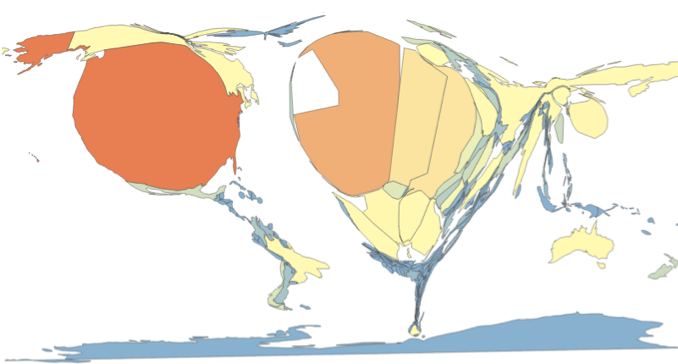
\includegraphics[keepaspectratio,width=\textwidth,height=0.75\textheight]{figures/wos_2012_cartogram.png}
\caption{Cartogram of Number of Journals in WoS in 2012}
\label{wos_cartogram}
\end{figure}

Other information systems like Scopus and Ulrich's Periodicals do not do significantly better. Looking at the figure above, the need for a ``comprehensive and reliable information system that duly gives account of the production of scientific periodicals [from Latin America]'' ~\citep[p. 91]{Cetto1998} becomes evident. This has been the motivation behind Latindex, an information system that has become the most inclusive and comprehensive source of information regarding scholarly journals in Latin America, the Caribbean, Spain and Portugal. Established in 1997, it is also the oldest of the three major scholarly communication information systems working at the regional level in Latin America.

There are two other major initiatives are working in the region: \href{http://www.scielo.org}{SciELO}\footnote{\href{http://www.scielo.org}{http:/\slash www.scielo.org}} and \href{http://www.redalyc.org}{RedALyC}\footnote{\href{http://www.redalyc.org}{http:/\slash www.redalyc.org}}, which collectively publish and index over 750,000 full-text articles from over 1300 journals.\footnote{These two initiatives are described in greater detail in the following chapter.} Unlike Latindex, these two initiatives are the source of information at the article level, not just the journal level. Although they operate quite differently from each other, they are both regional in nature, and could not be otherwise. For one, they both benefit from the economies of scale that come from working with hundreds of journals simultaneously, primarily by being able to attract readership from the entire region.

But, perhaps more importantly, these initiatives are actually better able to provide indexing and bibliometric services by taking advantage of the regional nature of Latin America's research activities.\footnote{While SciELO\slash RedALyC are technically publishers (that is, they ``publish'' content online which in some cases has not been made available elsewhere), they are not publishers in the traditional sense (i.e., they are not involved in the operation of the journals, do not provide financing, editing services, or any other oversight of the editorial or production process). They have also been described as a ``meta-publishers'' ~\citep{Packer2007} and as a hybrid between a repository and a publisher ~\citep{Guedon2008}.} For example, because most of Latin America's publications are still published in local languages and are often catered to a more local audience, they are more likely to receive citations from journals published locally. This is not the case for all regional publications, but it certainly is the case for some ~\citep{Meneghini2006,Collazo-Reyes2008,Collazo-Reyes2013}. There is also evidence of increased intra-regional collaboration between authors from Latin American countries (as evidenced by co-authorship) ~\citep{Lemarchand2011}. It is therefore of particular importance for a bibliographic service to capture citations and authorship from Latin American publications in order to provide citations and collaboration indicators, something which could not be done if the information service did not have broad coverage of regional journals.

That is, the initiatives are regional because the nature of Latin American scholarship exhibits regional characteristics, such as intra-regional citations and collaborations ~\citep{Meneghini2006,Collazo-Reyes2008,Collazo-Reyes2013,Lemarchand2011}. Although, there is great variability within the region, this evidence suggests that Latin America scholarly communications is a regional phenomenon. It is only by studying it as a such, that it is possible to assess the extent to which the reach and impact are, in fact, regional.

Just as with this study hopes to be, the initiatives have been more successful as bibliometric sources by being regional in scope. Of course, there have been many studies of study impact and reach, outside the Latin American context, that do not depend on such regional sources. An overview of such studies is presented in the following section.

\section{Bibliometrics, webometrics, and altmetrics}
\label{bibliometricswebometricsandaltmetrics}

Up until now, most of the work on evaluating alternative forms of scholarly journal impact on research (beyond citations) and of reach (usage) has been carried out in other contexts. Much of what has been learned may be generally applicable, or at least provides valuable lessons that can serve to understand the Latin American case. While working in a different context than the following studies, this work aims to contribute to the body of the bibliometrics and altmetrics communities, by exploring and expanding the existing methodologies and determining the universality of some of the existing claims. A brief overview of the research in this area is therefore presented below.

It serves to clarify the three terms used in this section heading: \emph{bibliometrics}, \emph{webometrics}, and \emph{altmetrics}. The former refers to a subfield of \emph{informetrics}, which  \citet[p. 1311]{Egghe2005} defines as ``as the broad term comprising all-metrics studies related to information science, including bibliometrics (bibliographies, libraries,…), scientometrics (science policy, citation analysis, research evaluation, …), webometrics (metrics of the web, the Internet or other social networks such as citation or collaboration networks).'' Bibliometrics is the oldest of the -\emph{metrics}, and is predominantly concerned with statistical analysis of the literature of science and scholarship ~\citep{Hood2001}. There is, of course, a lot more to the study of science and technology than what is published, which is where bibliometrics ends and scientometrics begins. The distinction between them is not always clear, and there has always been a great deal of confusion surrounding these terms.\footnote{A reader interested in the origins and definitions of these terms should consult Hood and Wilson's detailed description ~\citep{Hood2001}.} Somewhat more distinct is the middle term: webometrics.

\emph{Webometrics} is the ``quantitative study of Web-related phenomena'' ~\citep[p. 81]{Thelwall2006}. This subfield of informetrics emerged from the application of bibliometric techniques to the data produced from the linkages of the Web and from Web access logs ~\citep{Thelwall2006}. Webometrics has lead to the creation of new metrics such as Usage Impact Factor and the now famous click-through maps of science ~\citep{Bollen2009a}, but most recently through its extension (or subdivision) into altmetrics. Webometrics is a fairly well-established fields by now, having grown significantly as a field in the early 2000s ~\citep{Bar-Ilan2008b}. Despite its growth, there are some inherent challenges in working with Web data that have not been overcome, such as the reliance on search engines for data and the difficulties in obtaining and curating Web log (usage) data ~\citep{Priem2010d}. I return to some of the challenges with usage data in particular further down, as it bears on the present research.

The last term, \emph{altmetrics}, is the newest of the -\emph{metrics}. Altmetrics was originally coined in a Tweet ~\citep{Priem2010b} and subsequently described in the ``Altmetrics Manifesto'' as an extension of traditional bibliometrics to include the tracking of ``impact outside the academy, impact of influential but uncited work, and impact from sources that aren't peer-reviewed'' ~\citep[n.p]{Priem2010c}. As the field grows, new definitions have emerged, but they all propose, in varying levels of detail, examining the social Web as an alternative or enhancement to traditional bibliometrics (notably citation-based metrics like the Impact Factor) and of some of the metrics derived from the Web (such as download and usage data) ~\citep{Galligan2013a}.

Altmetrics are thought to capture a more ``nuanced'' notion of impact, by capturing when ``scholarly products are read, discussed, saved, recommended as well as cited'' and to provide ``indications of impacts on diverse audiences including scholars but also practitioners, clinicians, educators and the general public'' ~\citep[p. 9]{Piwowar2013}, aspects which are ignored by the bibliometric approach of evaluating impact ~\citep{Sud2011,Piwowar2013d,Costas2014}. Altmetrics work by looking for references to scholarly works on the Web, including ``traditional'' social media (i.e., Twitter, Facebook, Google+), blogs (i.e., researchblogging.com, ScienceSeeker, Wordpress.com), academic bookmarking services and reference managers (i.e., CiteULike, Mendeley, Connotea), media outlets (i.e., \emph{New York Times}, \emph{The Economist}, \emph{Wired}), and multimedia (i.e., Youtube, podcasts), post-publication peer review sites (i.e., F1000 Prime), and a handful of others. However, there is no official list of what constitutes an alternative metric. Virtually any metric that can be collected over the Web and that is not a citation is valid as an \emph{alternative} metric. Most altmetric providers are opting for collecting from as many sources as possible while the community gains a better understanding of what type of impact is captured by each.\footnote{The success of altmetric providers in identifying mentions of articles is varied and in some cases limited. For most sources there is a reliance on links, on the presence of unique identifiers (such as DOIs), or even the existence of an Application Programming Interface (API) to programmatically query the source. None of these methods is perfect, leading to data quality issues and variability between the providers ~\citep{Zahedi2014a}.}

A related development to both webometrics and altmetrics is the push towards Article-Level Metrics (ALMs), which call for impact to be evaluated at the article level, as opposed to the journal level. ALMs and altmetrics are sometimes confused, because ALMs often seek to incorporate alternative metrics. However, citation metrics (not alternative) are also an integral part of ALMs, and, conversely, altmetrics can be collected about any object, not just articles, and aggregated at different levels. In fact, altmetrics are also promoted for non-traditional research outputs such as datasets and software ~\citep{Piwowar2013a,Piwowar2013d}. A depiction of the relationship between altmetrics, ALMs, and journal-level metrics can be found in \autoref{alm_altmetrics_venn}.



\begin{figure}[htbp]
\centering
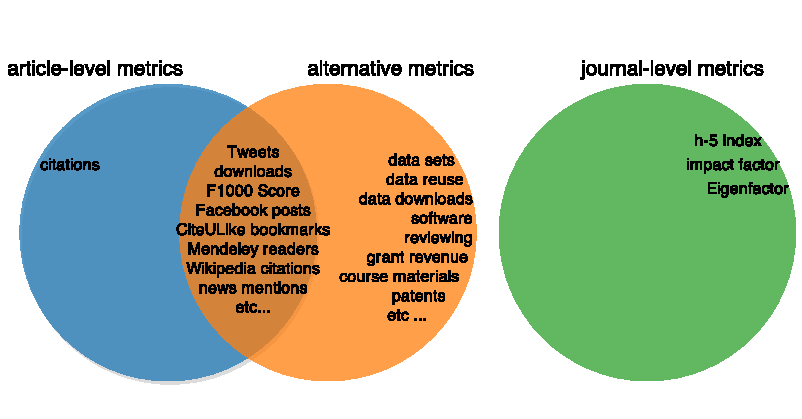
\includegraphics[keepaspectratio,width=\textwidth,height=0.75\textheight]{figures/alm_altmetrics_venn.pdf}
\caption{Relationship Between Article-Level Metrics and Altmetrics}
\captionsetup{font={footnotesize,bf,it}}
\caption*{(Source: Mulvany, 2004)}
\label{alm_altmetrics_venn}
\end{figure}



Proponents of altmetrics and ALMs share the common goal of wanting to move beyond the Journal Impact Factor (IF). One by looking at different metrics and the other by changing the object of study. Despite this common goal, it is perhaps unsurprisingly, given how established and well-studied and understood the IF is, that there have been numerous studies that compare the new metrics with the IF and to other citation measures. This is true just as much of usage (download) metrics as it is of the more recent altmetrics.

Bollen and colleagues have carried out extensive work in the field of usage impact measures, exploring what they have designated ``usage bibliometrics'' ~\citep{Kurtz2010}. While several studies have found positive correlations between article downloads and citations (either article citations or to the IF) ~\citep{Moed2005,Bollen2005,Brody2006}, there are two important caveats. First, usage and citations are understood to measure different dimensions of impact (even in the presence of a correlation), and therefore offer complementary information ~\citep{Bollen2009}. Second, the degree of correlation between the two measures appears to be influenced by the source of the usage data ~\citep{Bollen2008a}. For example, a data source stemming from a service that primarily serves a research community (such as the Los Alamos National Labs library system) may exhibit a stronger correlation to citations than one serving a community of undergraduates (such as the California State University system) ~\citep{Bollen2008a}. These differences stem from the \emph{span} and \emph{diversity} of the data source (i.e., how representative are the objects available through the data provider and how representative is the community accessing them through the data provider) ~\citep{Bollen2008a}. I address the representativeness of the OA portals in Latin America in the methodology section, where I claim that they are global in span (i.e., representative of all of Latin America) and extensive in terms of diversity (i.e., they attract all the relevant user types).

This problem with sample selection is already problematic when using a single source, but doubly so when trying to compare data across sources. Despite existing standards, such as COUNTER ~\citep{COUNTER2012} and PIRUS ~\citep{Shepherd2011}, issues such as journal interfaces continue to affect how users interact with content users, making even standardized reports difficult, if not impossible, to compare ~\citep{Davis2006}. In studies that rely on usage logs for download data (such as this one), it is also difficult to identify individuals, because IP addresses can change and some users rely on proxies (i.e., for off-campus access). However, projects like MESUR (Metrics from Scholarly Usage of Resources) ~\citep{Bollen2007} have successfully shown it is possible to overcome some of these issues ~\citep{Bollen2008}. Moreover, the use of Web logs has proven useful for a wide variety of studies, despite some of its limitations and challenges ~\citep{Jamali2005}.

The types of problems present with usage metrics are also present with altmetrics. As many have already discussed, data quality problems plague the field and are a barrier to the widespread adoption of altmetrics ~\citep{Haustein2013,Wouters2012,Costas2014}. However, as with usage metrics, data quality issues are not insurmountable and, even if it warrants cautions and caveats, the advantages offered by studying impact through these metrics are too many to be ignored, not least because of the growing importance of the role of the Web in the communication of science.

For example, Twitter use among scholars has been growing ~\citep{Priem2012}, and several surveys confirm that most scholars are making at least some use of ``Web 2.0'' tools ~\citep{Procter2010,Tenopir2013}.\footnote{Unsurprisingly, younger scholars seem to use social media more often ~\citep{Tenopir2013}. However, contrary to expectations, the respondents that report most social media use were also the ones who reported reading the most scholarly papers ~\citep{Tenopir2013}.} More generally, the number of articles that are shared or discussed each day is increasing at an estimated rate of between 5--10\% per month ~\citep{Adie2013a}. That is, the presence of articles in social media is still relatively low at an estimated 15--24\% ~\citep{Costas2014}, and even lower in Latin America as I demonstrate in Chapter 4, but the overall numbers are likely to increase over time.

So while we know that the presence of scholarly articles in online channels of communication is growing, what we still do not know is the degree to which altmetrics can be used for capturing impact. There is a definite sense that the numbers in some way indicate attention, influence, or even impact, but it is still unknown how. There are, as of yet, few large-scale studies and most altmetric research ends with a call for further study of the reliability, validity, and context of the available metrics ~\citep{Haustein2013,Wouters2012,Liu2013}.

Most altmetric studies so far have focused on the relationship between altmetrics and citation metrics. So far, the strongest correlation between an altmetric and citations were found for F1000 Prime recommendations ~\citep{Li2012}. However, several studies have shown a moderate level of correlation between saves in the bibliographic manager Mendeley and citations ~\citep{Li2012a,Priem2012,Bar-Ilan2012,Bar-Ilan2012a}. Mentions in blogs has also shown to have a positive correlation with citations ~\citep{Fausto2012b,Costas2014}, although this appears to be heavily influenced by the makeup of bloggers themselves and the journals they tend to blog about, both of which introduce a strong bias for high-impact life science journals ~\citep{Shema2012}. Twitter, the most prevalent of the social media altmetrics sources ~\citep{Thelwall2013c}, was found to have a low (but positive) correlation to citations ~\citep{Haustein2013,Eysenbach2011}.  \citet{Eysenbach2011} additionally found that highly tweeted papers could also be used as early predictors of citations, something supported by the findings of  \citet{Shuai2012a} and  \citet{Thelwall2013c}. In short, there appears to be a low to moderate correlation between altmetrics and citations, at least in the specific journals and disciplines studied (primarily well-known English-language natural and life science journals).\footnote{The following two recent papers also summarize many of the studies mentioned here and provide some details on sample sizes and correlation coefficients which are omitted here for brevity ~\citep{Haustein2013,Torres-Salinas2013}.}

However, most altmetric and usage studies also express that these new metrics capture a different ``dimension'', ``flavour'', or ``type'' of impact than citations ~\citep{Torres-Salinas2013,Costas2014,Haustein2013,Eysenbach2011,Bollen2008a,Bollen2009}. Not only are altmetrics and usage metrics different from citations, they are also different from each other ~\citep{Thelwall2013c,Bollen2009}. The implication is that altmetrics ``should not be considered as alternatives to citation-based indicators, but rather as complementary'' ~\citep[pp. 18--19]{Haustein2014b}.

It is precisely this finding, one of the main points of agreement between virtually all usage and altmetric studies, that justifies the continued exploration of altmetrics as a means of capturing impact. If they do capture a different dimension of impact than citations, then its possible that part of that impact is \emph{public} impact. This, however, remains to be studied. To date, what exactly is the impact uncovered by these metrics remains a mystery.

One of the keys to unlocking the mystery is to explore who is behind the metrics (i.e., who are the people sharing, bookmarking, and commenting on the research), something this study addresses by surveying users of social media directly, as some have been calling for ~\citep{Haustein2014b}.

In lieu of studies specific to those behind social media mentions of articles I rely on more general studies of online journal readers. A lot of what is known about readers of online journals, their reading habits and preferences, has been established by Carol Tenopir, Donald King, and their collaborators. This literature in this area primarily builds on the their early work, a series of reader surveys repeated over the years in several different contexts and dating back to 1977 ~\citep{Tenopir2000,Tenopir2009,Tenopir2010}. These early studies established many of patterns in readership that have since been corroborated by countless of other studies. Extensive summaries and reviews of these studies have been carried out elsewhere and are therefore not repeated here ~\citep{Tenopir2003,Rowlands2007b}. Instead, I focus on presenting several of their findings are germane to the present study.

 \citet{Tenopir2000} estimated that up to one third of journal readership coming from users who are not themselves authors (primarily students) and would therefore never appear in citation data ~\citep{Tenopir2000}. This is one of the important findings that justifies the search for \emph{alternative} forms of impact. A second important finding, one that has been replicated numerous times, is that users from different disciplines have different usage patterns and preferences ~\citep{Tenopir2000,Talja2003,Fry2004}. Other studies have extended this notion beyond disciplinary differences, leading to the conclusion that differences exists in usage patterns across other classes of users ~\citep{Tenopir2003,Fry2004}. For example, ``undergraduate students behave differently than do graduate students or faculty [and] searching for information for personal use is different from searching for work-related tasks'' ~\citep[p. 28]{Tenopir2003}. Evidence of different behavior has also been detected depending on whether users access an article from Google or Google Scholar (again, potentially indicative of a lay or public user versus an academic or otherwise experienced user) ~\citep{Kurtz2010}.

The above findings have two important implications for this study. One, they emphasize the importance of considering the disciplinary dimension in any analyses. Two, they provide a warrant for searching for different usage patterns from public and academic users in the available usage data.

Before delving into the methodological approaches that will be employed to attempt to suss out such differences, I present an unfortunately brief overview of what is currently known about Latin American impact and reach. Unfortunately brief because of the lack of research specific to the Latin American context.

~\nocite{Mulvany2014}

\section{Latin American impact and reach}
\label{latinamericanimpactandreach}

As can be seen from the bibliometric studies of impact and reach presented above, most of the work carried out in this field has been in contexts very different from Latin America. In most cases, the journals studied are well-known and well-established journals (i.e., Science and Nature) published in so-called ``developed'' countries (i.e., the US or Western Europe). They are predominantly subscription (non-OA) journals or, in a few cases, very large OA (mega-) publishers (i.e., PLOS and BioMedCentral). These studies have been invaluable in their contributions of methods, frameworks, and theories, but they are insufficient for understanding impact and reach in the Latin American context or for understanding the potential of OA more broadly.

In the following sections, I seek to present what is currently known about impact and reach of Latin American research. However, given the limited nature of the existing research, I stray beyond a literature review and put forth some very preliminary analysis carried out by me using data from SciELO and WoS. This analysis is, as of yet, rudimentary, but I present it here in the hopes to give the reader a better sense of what is currently known about impact and reach, even though so little has been formally published on the subject.

\subsection{Impact}
\label{impact}

Very little is actually known about the impact of Latin American journals overall. Despite the evident growth of the digital presence of Latin American journals, and of the extensive work carried out by the initiatives described above in cataloguing and tracking the work of Latin American journals, there have been only a couple of studies that examine their impact. Most of these studies, unfortunately, are very limited in scope and yield few (if any) generalizable results. For example, one study uses the SciELO citation data to rank business and economic journals ~\citep{Alexander2012}, while another study simply reports the IF for journals in the field of tropical and infectious diseases (the highest mean IF found for the period studied was 0.3500, and IF varied significantly from year to year) ~\citep{Rodriguez-Morales2009}. There are also numerous examples editors examining the citation ``Impact Factors'' of their own journals, some finding increased citation rates and others that they were in decline ~\citep{Pereira2006,Pinto2007,Huamani2009}. Another category of studies analyze articles with Latin American affiliations published in any journal ~\citep{Monge-Najera2012,Lemarchand2011,Holmgren:2004ij}. These latter studies are not as relevant for the questions being asked here, since they do not pertain to Latin American journals specifically and therefore do not shed any light on the citation impact of research published in publications from Latin America itself.

Before the creation of SciELO, the only source of citations of journals from developing regions were the WoS and Scopus—two databases that underrepresent the developing world.\footnote{Although the coverage of WoS and Scopus differs, the problem of underrepresentation of Latin American journals is the same. Several studies compare the coverage of Latin American journals in both ~\citep{Rodrigues2014,Miguel2011c} and one study found that key bibliometric indicators were equivalent ~\citep{Santa2010}.} Putting aside issues of equity, the underrepresentation and shear low number of journals from developing countries mean that journals that are geared towards the developing world will have less of its citations counted than one geared towards journals that are in the dataset. Its known, however, both by looking at the WoS ~\citep{Collazo-Reyes2008,Collazo-Reyes2013} and at SciELO (Brazil) ~\citep{Meneghini2006} that journals do precisely this. While some attract international citations, others appear to be geared towards local or regional audiences. As a direct consequence, their citations are simply not captured in the dataset and their resulting Impact Factors (IF) are kept artificially lower than they could be. As a consequence, the majority of Latin American journals have historically had their IF in the fourth quartile ~\citep{Luna-Morales2007,Packer2007}.

The problem is equivalent when looking at the citation counts calculated by SciELO (the difference, of course, is that SciELO is only capturing local and regional citations and omitting all those from outside the region). The partnership between SciELO and Thomson-Reuters, announced in October of 2013\footnote{http:\slash \slash thomsonreuters.com\slash press-releases\slash 102013\slash SciELO-Collaboration} aims to address this challenge by combining citations from the WoS and SciELO, but the data is not yet publicly available. Even so, this solution is not a panacea. Both databases, even when combined, continue to only provide a limited view of the citation impact of a developing region such as Latin America, and any studies using these data must consider this limitation.

There are, however, alternative measures of impact that are not affected by the overall coverage of the database of interest, as they are measures specific to each article, irrespective of the others in the dataset. These alternatives are explored in a following section, but first I ask: What is known about reach?

\subsection{Reach}
\label{reach}

As with impact, little is known about the extent to which research published in developing regions is circulated and read. To some degree, this is true of readership generally, not just in developing regions, despite an increased interest in usage-based metrics in the last decade. However, for developing regions, details on the demographics of the readership is of critical importance, as governments and funding agencies strive to focus their limited resources in serving their constituents.

Although download and view metrics are potentially available for every open access publication (by definition, an OA article must be online), there have been no systematic studies of usage patterns of Latin American journals. Most OA journals today do track users to some degree, either through dedicated systems or through standard Web analytic tools (i.e., Google Analytics). Yet, there has not been a project that aims to aggregate the metrics from each journal into a database that could be used to analyze journals together.\footnote{The ``Quality in the Open Scholarly Communication of Latin America'' project has actually sought to do this, but this aspect of the project it not yet complete ~\citep{Alperin2013e}.} There alternative is, as I propose to do here, to rely on journal portals that centrally collect download statistics for a large number of journals in a consistent manner between journals.

Both RedALyC and SciELO provide such usage statistics to the public. In the case of SciELO, they are only available for the Brazil collection. The RedALyC data, however, covers all of the journals. It is surprising that given the availability of these data, nobody has conducted a study analyzing different dimensions of downloads, beyond the overall view counts and ``top 10'' lists of articles available from time to time on the respective Web portals.

These data are available at the journal level from the Website and were made available at the article level for the purpose of this study, along with the corresponding article metadata, making it possible to draw further inferences about which journals, disciplines, and countries receive usage. An article-level analysis will lead to a clearer sense of where the audience of these OA journals is located and what content they are most interested in.

\section{Summary}
\label{summary}

The little that is known about the impact and reach offers few points of comparison to understand the situation of Latin American research. Despite the lack of a benchmark—a benchmark this study now hopes to establish—Latin American provides an ideal context in which to test the potential public impact of research more broadly. The broad adoption of OA, stemming from a historical context that is was receptive to knowledge as a public good and economic circumstances that kept scholarly publishing under control of public institutions, provides a continent of people who have an expectation that research will be readily and freely available to for their consumption. The regional approach to scholarly communication, stemming from a region's shared language, culture, and history, has manifested itself in intraregional collaborations and lead to the development of the large regional initiatives for OA publishing that are used in this study. The combination of both—widespread use of OA models and large regional initiatives—presents a natural experiment in scholarly publishing without which it would be impossible to test and draw meaningful conclusions regarding the reach and impact of research beyond the academy.

The development of the bibliometric, webometric, and altmetric approaches described above make it possible to study impact and reach in a multitude of ways. While some of the approaches have a long history and tradition, others, such as those that involve altmetrics have only been developed in the past five years. These new approaches have been made possible by increased presence of the social Web in our online lives, including in how we discover and read academic research. The few altmetrics studies that have been carried out have only indicated a sense that social media metrics may be useful for capturing non-citation based impact, but have not yet proven or otherwise quantified this potential.

It is by exploiting the combination of this context and these new approaches that this study seeks in to understand the alternative and public impact of research. The following chapter therefore describes the data and methods used to understand the impact and reach of Latin American research.

\chapter{Data and Methods}
\label{dataandmethods}

At its core, this study analyses the actions taken by readers of Latin American research and who those readers are. I examine who these users are: 1) through a series of pop-up polls that appear at the time of the download; 2) by examining the levels of access to Latin American research portals; 3) through the presence of article mentions and links on the Web; and 4) through a short survey conducted via Twitter. And while the users of the research are the centre of attention of this study, the main unit of analysis is the research article itself. And so download statistics, Web mentions, and author surveys will be linked a specific article (the one mentioned on the Web, or the one the that the user was downloading) and through that article to a subject field, a language, and a country of publication.

As such, all of the data used in this study, except the Twitter survey, can be said to be collected at the article level, even when it is about the people behind the usage. A broad range of article-level metrics, including usage data, altmetrics, and the user surveys, is used to better understand the nature and extent of the uptake, as well as the level of impact that individual articles, journals, disciplines, and countries from Latin America are having in the region and beyond.

This study draws on the two largest regional OA portals, RedALyC and SciELO. Through them, it accesses the data on thousands of articles and to the millions of readers of those articles. In the following sections I present an overview of these data, the data obtained through third parties, and the survey methodology employed. I subsequently go through the data analysis approach. Given the reliance on these two portals, I begin with a description of their coverage and the extent to which they represent Latin American journals more broadly.

\section{Sample selection}
\label{sampleselection}

There are actually many scholarly publishing initiatives in the region. They range from small and institutional, to large and regional (the ones I will be using), from broad multidisciplinary to subject specific, from those focused on scholarly journals, to those focused on institutional archiving, and they can be found in virtually every country between Mexico and Argentina. The number of initiatives continues to grow, but the three major initiatives, Latindex, SciELO, and RedALyC, provide the best available data on the scholarly publishing activities of the region.

I rely on the latter two, SciELO and RedALyC, for access to both articles and readers (Latindex does not host or publish content). It is precisely because these two initiatives are not a random sample that it is important to make explicit the extent to which these portals are representative of all journals from Latin America.

Although Latindex only has journal-level metadata (bibliographic information), it plays a critical role in the information ecosystem of scholarly journals in Latin America. Through co-operation with institutions of its 22 member countries (including all Spanish speaking countries in the region) Latindex maintains a \emph{comprehensive} catalog of 4,307 peer-reviewed journals.\footnote{Latindex also collects data about publications from Spain and Portugal, which are excluded from the numbers presented here. The Latindex Catalog is intended to be a selective list of journals that meet some basic editorial criteria, including but not limited to peer review. Details on the evaluation criteria can be found at: http:\slash \slash www.latindex.unam.mx\slash latindex\slash catalogo.html} While there are gaps in the coverage, and not all countries update their corresponding records with equal accuracy, completeness, or speed, the Latindex Catalog is the closest available proxy for the universe of publications from Latin America meeting a basic set of editorial criteria (including, among other things, peer-review). The Catalog therefore serves as a comparison set to explain the levels of representation of the data from SciELO and RedALyC.

SciELO and RedALyC both publish and index full-text articles for a combined total of over 1300 journals and over 750,000 articles.\footnote{See earlier footnote on how SciELO and RedALyC differ from traditional publishers.} They are widely recognized in the region ~\citep{Gomez2013} and have gained acceptance as markers of quality by several national science councils ~\citep{Alperin2011a}. Not only do they provide access to articles through their Web portals, but they curate all the metadata (bibliographic information), download data, and in the case of SciELO, citation data for the articles they publish. In short, they provide plentiful, rich data on scholarly journals published in the region. The best way to understand their level of coverage, however, is through comparisons to each other and to the master list of journals, the Latindex Catalog.

If we understand the Latindex Catalog as a description of the universe of journals from Latin America, we note that neither SciELO nor RedALyC are representative along some key dimensions. As we can see from the following tables, the coverage by subject varies greatly between the three Latin American sets (\autoref{subject_coverage}). Similarly, coverage by country also varies significantly by source \autoref{country_coverage}. In both cases, we see that neither SciELO, nor RedALyC provide coverage in proportions similar to those of in the Latindex Catalog (i.e., the percentage of coverage in SciELO and RedALyC do not match those of Latindex). As such, neither provide a representative sample of countries or subjects when compared to the Latindex Catalog. We also note that there is great variability between the lists.

We can see from these tables that the SciELO and RedALyC data are not a perfect representation of journals published in Latin America (i.e., not a random sample). Fortunately, the existence of the Latindex data as a point of comparison allows us to gain a sense of how representative journals studied are along these two dimensions (discipline and country).


\begin{table}[!htbp]
\centering
\caption{Number of Journals in Latin American Databases by Subject} \label{subject_coverage}
\begin{tabular}{@{}llll@{}}
\toprule
Subject               & Latindex       & RedALyC       & SciELO        \\ \midrule
Arts and Humanities   & 557 (12.93\%)  & 63 (9.03\%)   & 85 (9.48\%)   \\
Agricultural Sciences & 243 (5.64\%)   & 57 (8.17\%)   & 79 (8.81\%)   \\
Medical Sciences      & 768 (17.83\%)  & 91 (13.04\%)  & 235 (26.2\%)  \\
Natural Sciences      & 570 (13.23\%)  & 93 (13.32\%)  & 141 (15.72\%) \\
Social Sciences       & 2118 (49.18\%) & 394 (56.45\%) & 327 (36.45\%) \\
Engineering Sciences  & 286 (6.64\%)   & 61 (8.74\%)   & 62 (6.91\%)   \\
Multidisciplinary     & 323 (7.5\%)    & 28 (4.01\%)   & 13 (1.45\%)   \\ \bottomrule
\end{tabular}
\end{table}

\begin{table}[!htbp]
\centering
\caption{Number of Journals in Latin American Databases by Country} \label{country_coverage}
\begin{tabular}{@{}llll@{}}
\toprule
Country            & Latindex       & RedALyC       & SciELO        \\ \midrule
Argentina          & 473 (10.98\%)  & 41 (5.87\%)   & 110 (12.26\%) \\
Barbados           & 1 (0.02\%)     & -             & -             \\
Bolivia            & 19 (0.44\%)    & -             & -             \\
Brazil             & 1689 (39.22\%) & 154 (22.06\%) & 306 (34.11\%) \\
Chile              & 237 (5.5\%)    & 68 (9.74\%)   & 100 (11.15\%) \\
Colombia           & 504 (11.7\%)   & 154 (22.06\%) & 150 (16.72\%) \\
Costa Rica         & 97 (2.25\%)    & 15 (2.15\%)   & 15 (1.67\%)   \\
Cuba               & 129 (3\%)      & 22 (3.15\%)   & 48 (5.35\%)   \\
Ecuador            & 77 (1.79\%)    & 1 (0.14\%)    & -             \\
El Salvador        & 6 (0.14\%)     & -             & -             \\
Guatemala          & 4 (0.09\%)     & -             & -             \\
Honduras           & 3 (0.07\%)     & -             & -             \\
Jamaica            & 1 (0.02\%)     & -             & -             \\
Mexico             & 540 (12.54\%)  & 171 (24.5\%)  & 117 (13.04\%) \\
Martinica          & 1 (0.02\%)     & -             & -             \\
Nicaragua          & 6 (0.14\%)     & -             & -             \\
Panama             & 10 (0.23\%)    & -             & -             \\
Paraguay           & 15 (0.35\%)    & -             & -             \\
Peru               & 147 (3.41\%)   & 11 (1.58\%)   & -             \\
Puerto Rico        & 39 (0.91\%)    & 4 (0.57\%)    & -             \\
Dominican Republic & 16 (0.37\%)    & 1 (0.14\%)    & -             \\
Uruguay            & 56 (1.3\%)     & 2 (0.29\%)    & -             \\
Venezuela          & 237 (5.5\%)    & 54 (7.74\%)   & 51 (5.69\%)   \\ \midrule
Total              & 4307           & 698           & 897           \\ \bottomrule
\end{tabular}
\end{table}



\section{Data}
\label{data}

In the previous section I describe the two main sources of data used in this study, and the degree to which they can be used address questions about the extent and nature of the impact and reach of Latin American journals. In the sections that follow, I describe the specific data that is available at the article-level for this study, the additional data that was collected, and the methods by which it will be gathered.

\subsection{Article-Level data}
\label{article-leveldata}

As stated at the outset of this chapter, all of the data used for analysis in this study are calculated or otherwise linked to specific research articles. Most of the data, with the exception of that collected via surveys, is about articles themselves. This section describes those data as they pertain to this study.

Both portals gather detailed metadata at the journal and article level, including several fields that are used in this study: article identifier, title, year of publication, date uploaded and language, and journal country of publication and disciplines. These data are primarily from content published in the last decade, but also with some back-issues dating back many more, and can be used to slice and aggregate all article-level metrics.

Data from RedALyC was provided in a series of Excel files which were converted to CSV. There are a total of 204,453 articles, with the vast majority (98\%) corresponding to content published since the year 2000. Article data from SciELO was fetched through available APIs for the years starting in 2000.\footnote{Detail on the APIs can be found at http:\slash \slash docs.scielo.org\slash } Only articles from the Latin American SciELO portals was fetched, for a total of 389,795 articles, with Brazil making up 58\% of those articles.\footnote{The number of journals from each country in SciELO can be found in the previous section.}

To complement their bibliographic data, daily counts of full-text downloads are available for all of RedALyC and for the Brazilian collection of SciELO for downloads carried out during the 2013 calendar year. These usage statistics can be used for evaluating the frequency of access. Downloads are collected according to the COUNTER code of practice which attempts to filter out things such as non-human accesses and prevents double counting of downloads that are carried out in close succession (i.e., accidental double clicks) ~\citep{COUNTER2012}.

While the portals themselves have detailed metadata and download statistics, I rely on the largest of the altmetric providers, Altmetric.com for data from most altmetric sources, including social media (i.e., Twitter, Facebook, Google+), blogs (i.e., researchblogging.com, ScienceSeeker), academic bookmarking services (i.e., CiteULike, Connotea), and post-publication peer review sites (i.e., F1000 Prime). The data were provided in June 2014 and comprise all mentions in the above sources of any URLs within the SciELO or RedALyC domains (i.e., containing ``scielo'' or ``redalyc'' in the domain name). In the case of SciELO Brazil these data go back to January 2013, but in the case of the other SciELO domains and the RedALyC domain they begin in November 2013.

In addition, I rely on series of python scripts written by me to fetch the number of times articles are mentioned in the English, Spanish, and Portuguese editions of Wikipedia and saved in the Mendeley reference manager. Data from Mendeley was fetched by searching the Mendeley API with the article title, and verifying the search results using the year of publication and the first author last name.\footnote{https:\slash \slash github.com\slash jalperin\slash dissertation\slash blob\slash master\slash fetch\_mendeley.py} Wikipedia counts were fetched by searching for mentions of a partial URLs (specific enough to uniquely identify mentions of articles, but general enough to catch all URL variants of an article).\footnote{https:\slash \slash github.com\slash jalperin\slash dissertation\slash blob\slash master\slash fetch\_wikipedia.py} Both scripts were run between April and May, 2014.

These data were linked to the article metadata by extracting the article identifier from the URL mentioned in the Altmetric data with the identifier specified in the RedALyC and SciELO datasets. A randomly chosen record from the SciELO Brazil dataset, already combined with the Altmetric data, is depicted in \autoref{random_article_record}.



\begin{longtable}{@{}lp{5cm}p{6cm}@{}}
\caption{Sample Data Record}
\label{random_article_record} \\
    \toprule
    \multicolumn{1}{l}{Field} & \multicolumn{1}{p{5cm}}{Value}  &   \multicolumn{1}{p{6cm}}{Note} \\
    \hline
\endfirsthead

\multicolumn{3}{c}%
{{\tablename\ \thetable{} -- continued from previous page}} \\
    \hline
    \multicolumn{1}{l}{Field} & \multicolumn{1}{p{5cm}}{Value}  &   \multicolumn{1}{p{6cm}}{Note} \\
    \hline
\endhead

\hline \multicolumn{3}{r}{{Continued on next page}} \\ \hline
\endfoot

\bottomrule
\endlastfoot
id                 & S0104-66322013000300007                                                          & Unique identifier (specified by portal                               \\
publication\_date  & 2013-09                                                                          & Data of publication (with varying degrees of specificity)            \\
any\_issn          & 0104-6632                                                                        & Online ISSN if available, Print ISSN otherwise                       \\
journal\_title     & Brazilian Journal of Chemical Engineering                                        &                                                                      \\
journal\_url       & http://www.scielo.br{\slash}scielo.php?script=sci\_serial \&pid=0104-6632                &                                                               \\
authors            & Gris,L. R. S.; Paim,A. C.; Farenzena,M.; Trierweiler,J. O.                         & Authors, in order of publication                                    \\
original\_title    & Laboratory apparatus to evaluate microalgae production                           & Title in original language                                           \\
volume             & 30                                                                               &                                                                      \\
issue              & 3                                                                                &                                                                      \\
html\_url          & http://www.scielo.br{\slash}scielo.php?script=sci\_arttext \&pid=S0104-66322013000300007 &                                                              \\
original\_language & en                                                                               &                                                                      \\
subject\_areas     & Engineering, Exact and Earth Sciences                                      &                                                                           \\
downloads30        & 165                                                                              & Number of downloads in first 30 days since appearing online          \\
downloads90        & 378                                                                              & Number of downloads in first 90 days since appearing online          \\
mendeley           & 0                                                                                & Number of saves in Mendeley Reference Manager                        \\
en\_wiki           & 0                                                                                & Number of links found in English WIkipedia                           \\
es\_wiki           & 0                                                                                & Number of links found in Spanish WIkipedia                           \\
pt\_wiki           & 0                                                                                & Number of links found in Portuguese WIkipedia                        \\
wiki               & 0                                                                                & Number of links found in English, Spanish, and Portuguese WIkipedias \\
latindex\_subjects & Ciencias de la Ingeniería                                                       & Subjects according to Latindex                                       \\
Domain             & scielo.br                                                                        &                                                                      \\
news               & 0                                                                                & Number of mentions in major media outlets                            \\
blogs              & 0                                                                                & Number of mentions in science blogs                                  \\
twitter            & 1                                                                                & Number of Tweets                                                     \\
peer\_reviews      & 0                                                                                & Number of reviews  in external peer-review sites                     \\
facebook           & 0                                                                                & Number of mentions on public Facebook wall posts                     \\
googleplus         & 0                                                                                & Number of mentions in Google+                                        \\
linkedin           & 0                                                                                & Number of mentions in LinkedIn                                       \\
reddit             & 0                                                                                & Number of mentions in Reddit                                         \\
pinterest          & 0                                                                                & Number of mentions in Pinterest                                      \\
f1000              & 0                                                                                & Number of mentions in Faculty1000                                    \\
q\&a               & 0                                                                                & Number of mentions in Q\&A sites                                     \\
video              & 0                                                                                & Number of mentions in videos                                         \\ \end{longtable}



\subsection{Surveys}
\label{surveys}

Even though the article data gathered by SciELO, RedALyC, and through the altmetrics services, is extensive, it is not sufficient for understanding the demographics of the users of Latin American research. I therefore complemented these data with online polls (surveys). The goal of these polls is to gathering a demographic profile of the readers that use these portals. In this section, I describe the questions that were asked in the surveys, the purpose for asking them, and the strategy employed to collect the responses.

The research questions being investigated through this study call for a greater understanding of \emph{who} the readers of Latin American research are. While download statistics can provide a sense of the volume of readers, and the subjects they are interested, in they do not give us a sense of of the characteristics of the readers themselves. I therefore delve into the reader characteristics by displaying a series of ``pop-up'' question to users \emph{at the time} they download an article.

\subsubsection{Pop-up surveys}
\label{pop-upsurveys}

The pop-up surveys displayed at the time of download are the primary instrument for collecting data about the readers. The idea of linking survey responses to a ``critical incident'' (the last article the user read) has been used for print and online surveys previously ~\citep{Tenopir2000,Tenopir2010}, but doing so at the time of the download itself has the added advantage that the critical incident does not need to be self-reported. The online nature of the survey automatically captures the incident and allows for it to be analyzed along with other data about the article. This methodology also ensures that all types of readers, not just those form within the academic community, are exposed to the surveys as it does not rely on mailing lists or other form of participant identification.

By polling the reader while they have the article of interest in front of them, the URL and the ID of the article in question are captured automatically. Although, ideally I would be able to ask any number of questions to each person visiting the portals, it is known that response rates of pop-up surveys tend to be low (a summary of several studies suggests that it hovers around 20\%) ~\citep{Couper2001} and that additional questions tend to make it worse ~\citep{Comley2000}. Given the low-response rates of such polls and Web surveys generally, it is important to use single-question pop-ups that can be answered quickly. These single question polls are quick for a user to respond (almost as quick as closing the pop-up). A sample pop-up can be seen in \autoref{pop-up_survey_sample}.

\begin{figure}[htbp]
\centering
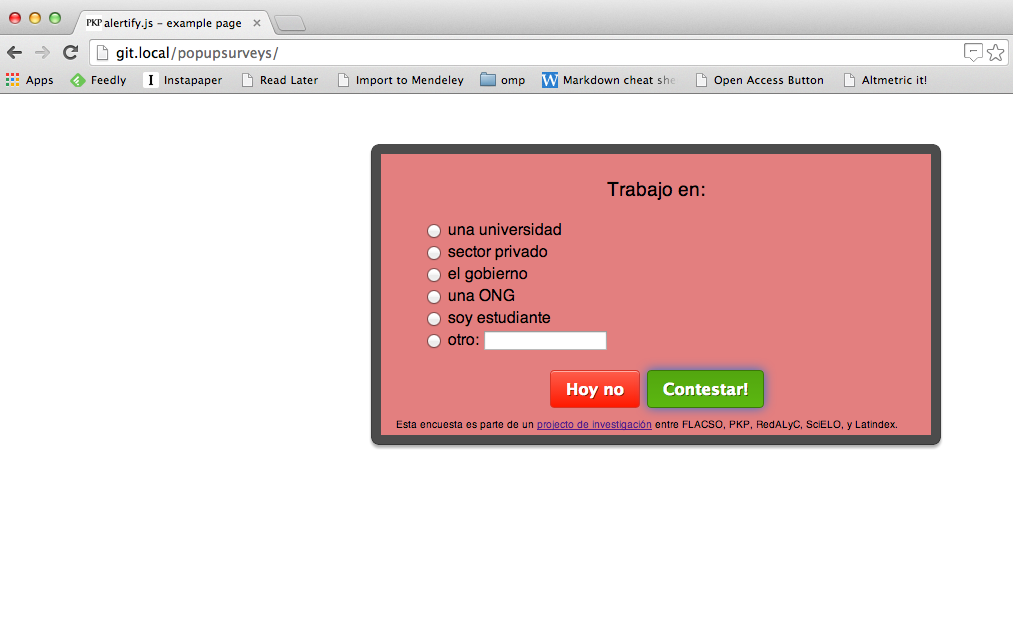
\includegraphics[keepaspectratio,width=\textwidth,height=0.75\textheight]{figures/pop-up_survey_sample.png}
\caption{Sample Pop-up Survey}
\label{pop-up_survey_sample}
\end{figure}

In general, coverage error (not reaching the target population) ``is presently the biggest threat to inference from Web survey'' ~\citep[p. 467]{Couper2000}. However, in this case, the target population is the people who access the journals published in the Web portals. Hence, validity of the results primarily rests on getting a high response rate (non-response error), to a void a bias against those that do not participate in surveys (who are sometimes different along some dimensions from those that do) ~\citep{Couper2000,Vaske2008}. To measure to response rate, the pop-up software assigns a unique identifier to each visitor (by setting a ``cookie'' in the browser) and tracks every identifier that is displayed a question, regardless of whether they respond or not. Response rates were not calculated for each individual question, but rather by calculating the ratio of respondents to the number of individuals who were shown a question. The result was a very high overall response rate of 38\% on the RedALyC portal (69,945 respondents out of a potential 183,369) and a remarkable 49\% on SciELO (175,757 respondents out of a potential 358,804).

\subsubsection{Conditions for displaying pop-ups}
\label{conditionsfordisplayingpop-ups}

Surveys were collected on RedALyC, and on three of the SciELO portals (Brazil, Mexico and Chile) between March and July 2014. During this period, a javascript code was inserted onto the page that displayed full-text of articles, which would trigger a pop-up with a 1 in 1000 chance after the person remained on the page for at least 10 seconds (enough to ensure a human visitor and a a non-accidental visit). The probability of choosing the pop-up was chosen as a compromise in not displaying too often, which would be disruptive to the operation of the portals, and too infrequently, which would bias the sample towards more frequent visitors ~\citep{Comley2000}.

Once the pop-up was triggered, one of the questions below was chosen at random. The targeted user users would not be surveyed again (whether they respond or not). The lack of repetition was controlled through browser cookies which, in theory, any user could disable or clear but, in practice, very few users do.\footnote{Even with cookies disabled or cleared, the probability of seeing the same question twice is extremely low, because the probability of being chosen twice is already very low (1 in 1,000,000).} Responses were sent to a Google Spreadsheet for online storage and downloaded on a weekly basis.

\subsubsection{Pop-up questions}
\label{pop-upquestions}

Each pop-up would contain, with equal probability, one of the following four questions, or a link to a short demographic survey. Questions were displayed in the language of the article being looked at, or in the language chosen by the user if they had altered the language of the user interface.



\begin{enumerate}[label=Q{\arabic*}:,nosep]
    \item
        I am interested in this article for …
        \begin{enumerate}[label={\alph*}),nosep]
            \item
                my job at a university
            \item
                my job at a research centre
            \item
                my job in the private sector
            \item
                my job at an NGO
            \item
                my job in government
            \item
                a class (I am a student)
            \item
                out of personal interest
            \item
                other \_\_\_\_\_
        \end{enumerate}
    \item
        I am interested in this article because I am doing research for ...
        \begin{enumerate}[label={\alph*}),nosep]
            \item
                academic reasons
            \item
                professional reasons
            \item
                personal reasons
            \item
                I am not doing research
        \end{enumerate}
    \item
        I work in ...
        \begin{enumerate}[label={\alph*}),nosep]
            \item
                a university
            \item
                I am a student
            \item
                the public sector
            \item
                the private sector
            \item
                the non-profit sector
            \item
                I am currently not working
            \item
                other \_\_\_\_\_
        \end{enumerate}
    \item
        Do you usually share articles on social networks? (you can choose more than one response)
        \begin{enumerate}[label={\alph*}),itemsep=0pt,parsep=0pt]
            \item
                NO
            \item
                Yes, on Facebook
            \item
                Yes, on Twitter
            \item
                Yes, on Mendeley
            \item
                Yes, on blogs
            \item
                Other
        \end{enumerate}
    \item
        Would you help us by answering a brief survey (less than 2 minutes)?
        \begin{enumerate}[label={},itemsep=0pt,parsep=0pt]
            \item
                For this question, users were offered a link to participate in a short demographic survey. This survey contained only four questions: level of education, age (in 5-year increments), sex, and employment sector. The employment sector question was identical to question 3 above.
        \end{enumerate}
\end{enumerate}



\subsubsection{Twitter survey}
\label{twittersurvey}

The final instrument used to collect information about the users is a brief survey conducted over the online social network Twitter. Using the Altmetric.com data, the screen-names of 6397 Twitter users who either Tweeted or Retweeted a link to an article published by SciELO Brazil sometime in 2013 were identified.

A Twitter account with the screen name @AcademicOrNot was set up, identifying itself as a research account owned by me (Twitter screen name @juancommander). Using an automated program, a Twitter status update (a Tweet) was posted every two minutes `mentioning' in random order each of the identified accounts. Mentions are ``any Twitter update [Tweet] that contains `@username' anywhere in the body of the Tweet'' ~\citep[n.p.]{Twitter2015}. These mentions cause the Tweet to appear in the ``mentions'' and ``notifications'' tabs of the person mentioned, alerting them to the Tweet ~\citep{Twitter2015}. All Tweets were made over a period of 11 days starting on March 21, 2015.

Because the identified accounts had Tweeted a link to an article from SciELO Brazil, which publishes primarily Portuguese articles, the survey was conducted in Portuguese, regardless of the language of the downloaded article. Every Tweet sent contained a text that translates to ``This is a survey by @juancommander, please help by responding: Are you affiliated with a university? Thank you @$<$screen\_name$>$!''. Responses were collected until April 30, 2015, although most responses arrived within a week of the question being sent. Of the 6397 accounts that had shared an article from SciELO Brazil, approximately 5\% were not longer active, leaving 6093 successful messages being sent out. Of these, only 286 responded, corresponding to a 5\% response rate. This low response rate is not surprising, given that messages were unsolicited, over a medium that where this type of message is uncommon, and in some cases, in a language that the recipient may not be familiar with. Even though it may provide limited representativeness, it still allows for a glimpse of the individuals on whom the research has had impact.

Users that responded to the survey question in the affirmative, were asked a single follow-up question: ``Are you a student, or do you work for the university?''. Those that responded in the negative were asked ``What line of work are you in?'' Responses were saved and coded as ``Not affiliated'', ``Affiliated - Student'', ``Affiliated - Faculty\slash Staff'', or ``Affiliated - Unspecified\slash Organization''. The latter category was chosen when an initial response the affirmative was received, but no response was received for the follow-up question or in the few instances where the account belonged to an academic organization

\subsection{Summary}
\label{summary}

In summary, the level of data available at the article-level regarding the publications themselves is extensive. These two OA portals host hundreds of thousands of articles across many disciplines and from all over Latin America. In terms of usage, we already know that they attract millions of visitors each year and for this study, detailed download data was made available for downloads that took place during the 2013 calendar year. With respect to other metrics, this study uses detailed data collected by Altmetric.com and through a couple of self-administered python scripts. Finally, information on readers was collected through a series of pop-up polls (surveys) that were collected at the time of download, and a short Twitter survey was conducted of users identified from the Altmetric.com data. The sources and overview of the available data can be found in \autoref{summary_of_data}. This is a unique and well-suited set of data for assessing impact at the article-level.

\begin{figure}[htbp]
\centering
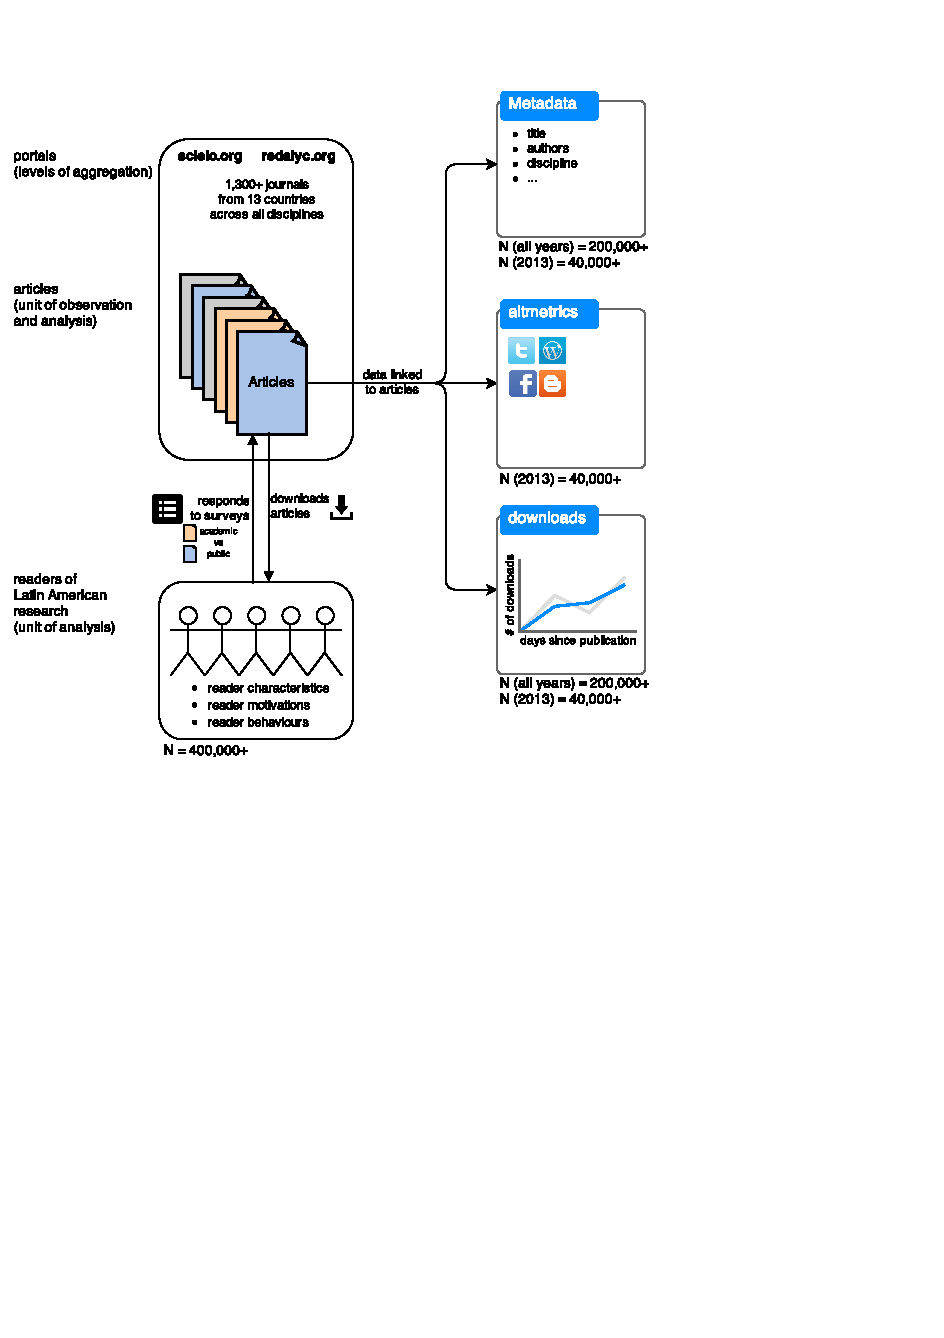
\includegraphics[keepaspectratio,width=\textwidth,height=0.75\textheight]{figures/summary_of_data.pdf}
\caption{Summary of Data Available}
\label{summary_of_data}
\end{figure}

\section{Methods}
\label{methods}

This study is primarily exploratory. As such, it relies heavily on descriptive statistics and data visualizations that seek to elucidate the nature of the impact and use of Latin American research, as seen through the two major portals described. The methodology is therefore straight forward: data is collected and described in detail using simple statistics such as means, standard deviations, proportions, etc. In the majority of cases, it is broken down by different dimensions such as country, discipline, and language, and the relationships between dimensions is described. Where appropriate, correlations are calculated between dimensions. The only exception to this descriptive approach is in the creation of topic models, as will be described later in this section.

Unless otherwise stated, all such statistics were calculated in Python using the Pandas package version 0.15.\footnote{http:\slash \slash pandas.pydata.org\slash } All Python scripts used for data manipulation can be found on online, although some of the results were obtained through interactive programming can therefore not be made available offline.\footnote{https:\slash \slash github.com\slash jalperin\slash dissertation\slash }

The data for the Surveys were collected using custom javascript code and the responses were sent programmatically to a series of Google Spreadsheets that were downloaded weekly as a comma separated file (CSV).\footnote{https:\slash \slash github.com\slash jalperin\slash popupsurveys} Survey data was linked to article data by extracting the article ID from the URL at the time the user responded to the survey and linking to the datasets provided by SciELO and URL. Questions were standardized to the English responses. The free-text responses were categorized as ``other'' for all questions for the purposes of the analyses presented here.

In all cases, data was limited to data from Latin American and Caribbean countries, even when the portals made data from outside the region available. Although surveys were not restricted to these countries, all responses from outside Latin America and the Caribbean were filtered out and are not included in the analyses or the calculation of response rates.

The approached followed was exploratory, beginning with the question at the heart of this study: who accesses Latin American research? This question is primarily answered by analyzing the demographic and pop-up surveys employed on the research portals. These were looked at as overall percentages of each response, and subsequently broken down by country of publication, discipline, and language. Because each of these subcategories were present in varying proportions in the portals studied, the results are presented as proportions of each of the categories. To facilitate comparisons and interpretations of significance, error bars included in the figures. Error bars are calculated based on the standard error for proportions, defined as the square root of p(1-p)\slash N, where p is the proportion reported and N is the number of responses.

In an attempt to gain a more granular understanding of disciplinary breakdowns, a series of ``topic models'' were run that help to identify the terms that commonly co-occur between a set of articles. In this study, I use a class of probabilistic models known as latent Dirichlet allocation (LDA) models ~\citep{Blei2003} to identify these sets of words. In these models, topics are ``a specialized probability distribution over words'' and ``a topic model specifies a probabilistic procedure by which documents can be generated'' ~\citep[p. 610]{McFarland2013}.

Because of our interest in comparing topics for different respondents, I use a sub-class of these models known labelled LDA (L-LDA) that can be used to assign multiple labels to each document. L-LDAs model every document as a combination of both words (the article's title) and labels (the survey responses) by assigning words to labels ~\citep{Ramage2009,McFarland2013}. Instead of a single probability distribution of words, like is the case in LDAs, the result of L-LDAs is a set of distributions, one for each label (survey response). These distributions can then be compared to each other using a cosine similarity score.\footnote{Cosine similarity is calculated by taking the cosine of the angle between two n-dimensional vectors, where n is the number of terms in the model. Two vectors oriented in the same way (where the same terms are prevalent in the same proportions) will have a cosine score of 1 (their angle is 0). Two vectors that are orthogonal to each other will have a cosine score of 0 (their angle is 90).}

L-LDA models were calculated using the Stanford Topic Modeling Toolkit on the basis of CSV files extracted from the datasets in question.\footnote{http:\slash \slash nlp.stanford.edu\slash software\slash tmt\slash } Each article was represented only by its title, in the original language of publication, with all non alpha-numeric characters removed. All diacritical marks were moved using NFKD normalization, which converts letters with diacritical marks to their ASCII equivalent (i.e., é becomes e, ñ becomes n, ã becomes a, etc.).\footnote{https:\slash \slash docs.python.org\slash 2\slash library\slash unicodedata.html\#unicodedata.normalize} Common words from English, Spanish, and Portuguese were removed using the list of ``stop words'' provided by Python's Natural Language Processing Toolkit (NLTK) Wordlist Corpora.\footnote{http:\slash \slash www.nltk.org\slash book\slash ch02.html\#fig-lexicon}

Graphs and other visualizations were made through a combination of the javascript library d3.js, Python's Matplotlib (used directly or through Pandas), and Excel.

\chapter{Results}
\label{results}

The resulting analysis presents a cross-section of the reach and impact of Latin American research as seen through the two portals studied. Since this study seeks to understand the readers of Latin American research and the impact that research published in Latin America has on these readers, the analyses is necessarily grounded in the demographics of who these readers are, what research they are reading, and the extent of that reach.

The chapter therefore begins with these demographics of readers of research published in Latin America, and combines these with their reasons for accessing the research, the topics they are interested in, and the extent of the reach of the research.

After showing that the audience of Latin American journals is primarily non-authors (who would not produce citation impact), the second half of this chapter concludes with a first exploration of the impact of Latin American research using alternative measures (altmetrics). This analysis covers the two portals, but because it is primarily an exploration of the potential of measures that are not yet widespread, it focuses special attention to the region's largest country (Brazil).\footnote{A significant portion of the latter half of this chapter has been previously published in  \citet{Alperin2015b}.}

Because this study is intended to provide a benchmark of the reach and impact of Latin American research, all data are presented in detail, and broken down by different dimensions, even when there is no discernible pattern. This way, should differences emerge in future studies, this chapter will have a documented point of comparison. Some readers may prefer to skip to Chapter 5, where the key insights and results from this chapter are summarized and discussed in detail, along with their implications.

\section{Reach}
\label{reach}

The following section therefore begins with an overview of the pop-up survey results and the short demographic survey that gives us a sense of who the readers are. These are straight forward descriptions, but they provide a sense of the demographics of users, and a picture of the reasons why they read content from the Latin American portals. Because their responses are linked to specific articles, they allow for the exploration of results across key dimensions, such as the original language of the article, the country of publication of the journal, and the subject classification.

The exploration of responses across subjects leads to the creation of topic models that allow a finer grained description of the subject matter being accessed. A labeled topic model, using each response as a label, allows for comparison in the similarity of the content being accessed across responses.

While these two sections provide a good sense of who readers are and what they are reading, they do not give a sense of the extent of the reach that the Latin American journals have. By looking at download counts, it is possible to see the number of downloads that these journals receive, but also to compare the average number of downloads that articles from each of the response categories receives.

\subsection{Demographics}
\label{demographics}

The most fundamental question to understand the reach of Latin American research is ``who are the users of this research?'' As such, the results presented below cover the demographics for those readers and articles sampled, including breakdowns by place of work, gender, interest in an article, and by the article's characteristics. Taken together, this data describes the characteristics of those who reach for Latin American research. By way of summary, there can be said to be three main types of readers: Students, Academics, and the Public (\autoref{reach_summary}). This composite summary of the article readership is a key result, challenging the assumption that academics write for academics (and assumed by academics as much as anyone). It challenges assumptions about students reading original research (rather than textbooks). It challenges the assumption that the public has no interest or capacity for research (although this study does not investigate the nature of this public use). A further distillation and discussion of key results can be found in Chapter 5, after a detailed breakdown and analysis of the data accumulated by this study.



\begin{table}[!htbp]
\centering
\caption{Summary of Users Reached} \label{reach_summary}
\begin{threeparttable}
\begin{tabular}{@{}lllll@{}}
\toprule
Type of Reach     &\multicolumn{2}{c}{Approximate Proportion} \\ \cmidrule{2-3}
    &   SciELO  &   RedALyC \\ \midrule
Students    &   50\%    &   55\%    \\
Staff (including faculty)   &   25\%    &   22\%    \\
Professional    &   20\%    &   17\%    \\
Personal    &   9\% &   6\% \\ \bottomrule
\end{tabular}
\begin{tablenotes}
\small
\item Note: This table represents a composite of the results presented in this chapter, derived from the author's interpretations of the data. As such, the numbers should be treated only as approximations, and the percentages should not be expected to add to 100\%.
\end{tablenotes}
\end{threeparttable}
\end{table}



In looking at the survey responses in more detail, the demographics of the readers of both portals are of central importance. The four-question demographic surveys, linked from a pop-up poll, provides valuable insight into the general make-up of the audience by examining the users' level of education, gender, age, and sector of employment. Unlike the pop-up polls, which by design, only presented each users with a single question, the demographic surveys allow the data to be pivoted across the four dimensions so that relative proportions can be calculated (see \autoref{demographic_parallel_coordinates_redalyc} for summary of RedALyC responses and \autoref{demographic_parallel_coordinates_scielo} for a summary of SciELO's).\footnote{The length of the black line indicates the percentage of respondents, whereas the colour `flows' show the breakdown of each response relative to the row above and below. Interactive versions of these charts can be found at: http:\slash \slash alperin.ca\slash dissertation\slash  which reveal the percentages on hover, and allow the order of both the questions and responses to be rearranged.} A surprising degree of similarity between the demographic surveys in both portals provides some confidence in the numbers gathered.\footnote{However, it should be noted one of the survey questions was also asked as a single pop-up poll (Q3) and, in both portals, the numbers varied between the survey and the pop-up polls. The pop-up responses are analyzed in detail below and the pop-up responses to Q3 can be found in \autoref{q3_summary}.}

Key to understanding the alternative forms of impact of Latin American research are the sectors in which readers of the research are working in. The surveys reveal that, in fact, the primary users of the portals are students, making up 47 and 42\% of RedALyC and SciELO respectively (almost 90\% of these have either a High School education or a Bacherlor's degree, but more on this below). University employees (not necessarily faculty) are the second largest set of users, making up the 20\% of all users in both portals. Public, private, and non-profit sector employees make up 16, 14, and 11\% of RedALyC and 11 and 12, and 2\% of SciELO. Other respondents (including those who are unemployed) make up 4 and 6\% of RedALyC and SciELO respectively.\footnote{In the pop-up version, fewer proportions reported working in the three non-academic sectors and more reported being students (although the proportions between sectors remain unchanged).} While these numbers show that the majority of users do come from from within academia, they also reveal that the majority are students (not employees, as might be expected) and that there is a significant number of users who work outside universities.

The highest level of education attained is also revealing, especially when crossed with the responses from the employment sector above. First, 22\% of users in both portals have only completed high school, and of these, around 80\% of them report being students (presumably, undergraduate students). Those with completed Bachelor's degree (or equivalent) make up the largest of the education-level groups at 46 and 42\% of all users of RedALyC and SciELO respectively. Around 50\% of these are themselves students (presumably, graduate students). The remainder of the students have completed Master's degrees, and very few have doctorates. This suggests that the student population, which makes up over 40\% of users of both portals, is split fairly evenly between undergraduate and graduate students.

The second largest cohort, university employees (22\% of the total), is made up primarily of university-educated individuals. Almost 90\% of these have completed at least a Bachelor's degree (roughly 25\% of have a Bachelor's, 35\% a Master's, and 30\% a PhD) (\autoref{demographic_work_education_pivot_redalyc} and \autoref{demographic_work_education_pivot_scielo}). While only 30\% of those that work at universities have a PhD, the majority of users with a PhD's work at universities (70 and 60\% of RedALyC and SciELO users respectively). This subsection of the population, individuals with doctorates that work at universities (i.e., the typical university professor) only make up 5--6\% of the total users.

Although the university-affiliated workers make up the largest portion of the users of the two portals, there is still a large portion of the population that works outside of the universities. This population which makes up around 35\% of those surveyed, is largely university-educated, with just over 50\% of those employed in the three non-academic sectors holding a Bachelor's degree, approximately 30\% holding a Master's degree, and between 6 and 9\% holding a PhD (RedALyC and SciELO respectively) (\autoref{demographic_work_education_pivot_redalyc} and \autoref{demographic_work_education_pivot_scielo}).

\begin{figure}[htbp]
\centering
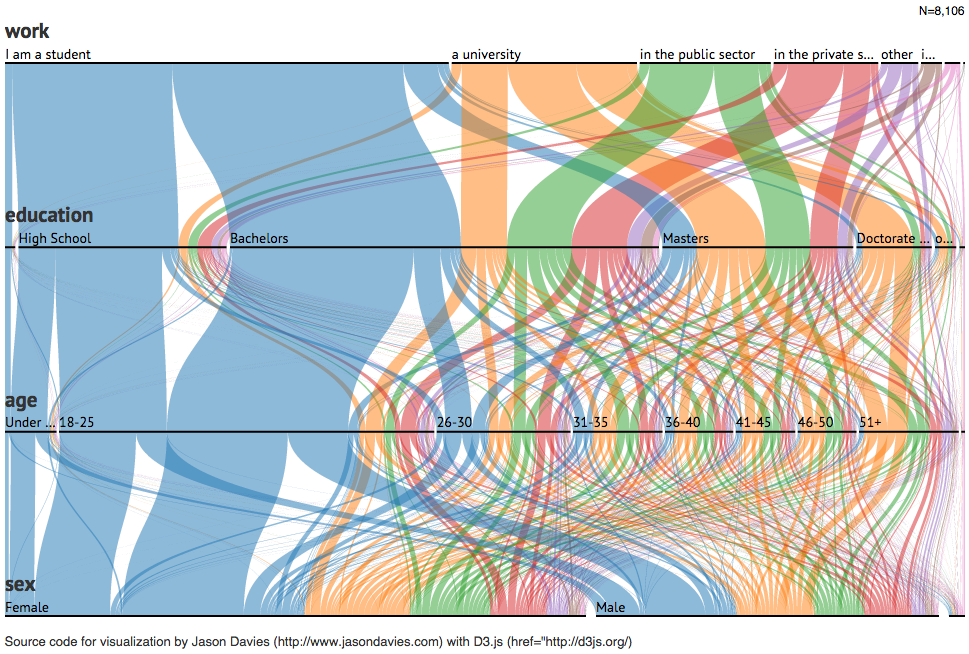
\includegraphics[keepaspectratio,width=\textwidth,height=0.75\textheight]{figures/demographic_parallel_coordinates_redalyc.png}
\caption{Demographics of SciELO Users}
\label{demographic_parallel_coordinates_redalyc}
\end{figure}

\begin{figure}[htbp]
\centering
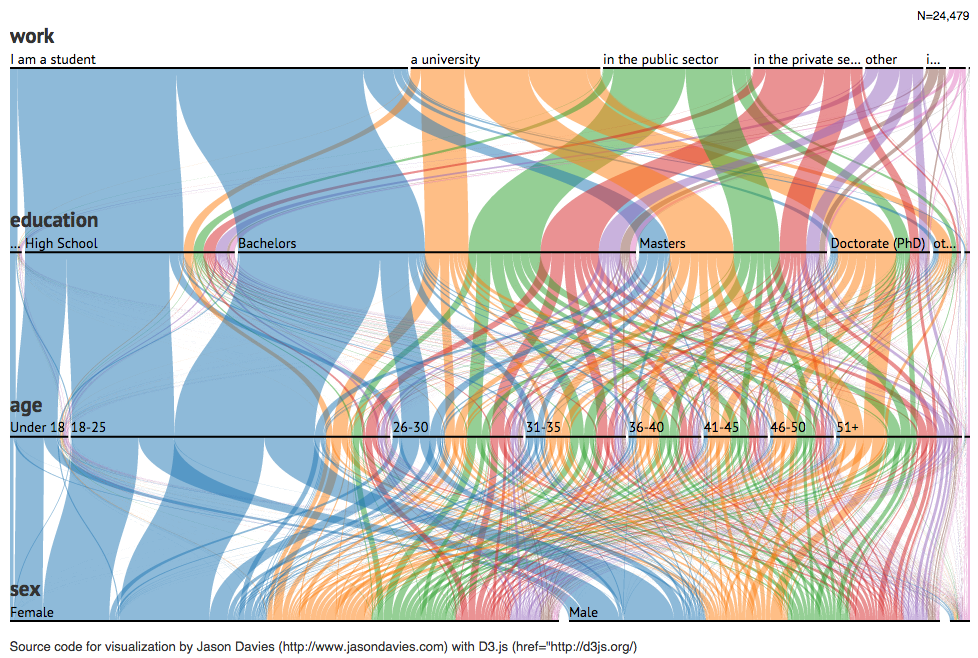
\includegraphics[keepaspectratio,width=\textwidth,height=0.75\textheight]{figures/demographic_parallel_coordinates_scielo.png}
\caption{Demographics of SciELO Users}
\label{demographic_parallel_coordinates_scielo}
\end{figure}



\begin{sidewaystable}[!htbp]
\centering
\caption{RedALyC user education level breakdown by employment sector} \label{demographic_work_education_pivot_redalyc}
\begin{tabular}{@{}llllllll@{}}
\toprule
    &   Elementary  &   High School &   Bachelors   &   Masters &   Doctorate   &   Other \\ \midrule
I am a student  &   1.65    &   36.15   &   52.21   &   7.79    &   1.31    &   0.89    \\
A university    &   0.25    &   5.16    &   25  &   37.22   &   27.46   &   4.91    \\
In the non-profit sector    &   1.1 &   14.36   &   55.25   &   22.65   &   5.52    &   1.1 \\
In the private sector   &   0.22    &   13.36   &   53.45   &   26.28   &   4.12    &   2.56    \\
In the public sector    &   0.35    &   7.18    &   49.2    &   34.13   &   6.03    &   3.1 \\
I am not currently working  &   0   &   18.75   &   62.5    &   18.75   &   0   &   0   \\
Other   &   2.54    &   17.46   &   38.1    &   26.98   &   12.38   &   2.54    \\ \bottomrule
\end{tabular}

\vspace{2\baselineskip}

\caption{SciELO user education level breakdown by employment sector} \label{demographic_work_education_pivot_scielo}
\begin{tabular}{@{}llllllll@{}}
\toprule
    &   Elementary  &   High School &   Bachelors   &   Masters &   Doctorate   &   Other \\ \midrule
I am a student  &   1.89    &   39.99   &   47.18   &   7.68    &   1.90    &   1.36    \\
A university    &   0.22    &   5.18    &   23.01   &   33.72   &   30.85   &   7.01    \\
In the non-profit sector    &   0.77    &   12.09   &   49.52   &   28.21   &   7.49    &   1.92    \\
In the private sector   &   0.49    &   11.16   &   53.48   &   24.37   &   8.51    &   1.98    \\
In the public sector    &   0.42    &   6.73    &   48.96   &   31.31   &   9.36    &   3.23    \\
I am not currently working  &   2.86    &   31.43   &   45.71   &   8.57    &   11.43   &   0   \\
Other   &   3.01    &   20.07   &   37.19   &   22.94   &   14.11   &   2.68    \\ \bottomrule
\end{tabular}
\end{sidewaystable}



Breaking down level of education by age groups yields unsurprising results. Those below 25 years of age are extremely likely to be students, a trend that diminishes as the individual gets older. Each of the work sectors, however, are all made up of individuals from across the age groups in fairly even numbers. This balance is not replicated across gender, where we see an overall predominance of women users in both portals (making up 62\% of RedALyC respondents and 58\% of SciELO respondents).

The predominance of women also holds across work sectors, with student respondents driving up the average with over 65\% female in both portals (\autoref{demographic_work_gender}). The only exception is the private sector, which appears to be more gender-balanced than the rest. Across education levels, women form the majority of readers with approximately a 60--40 male-female split for all levels (\autoref{demographic_education_gender}). The only exception here are those individuals with doctorates, whose group is more gender balanced than the rest.



\begin{table}[htbp]
  \centering
  \caption{Latin American portal user gender breakdown by employment sector} \label{demographic_work_gender}
  \label{demographic_work_gender}
    \begin{tabular}{@{}lllll@{}}
    \toprule
          & \multicolumn{2}{c}{SciELO} & \multicolumn{2}{c}{RedALyC} \\
          & \multicolumn{2}{c}{N=23,709} & \multicolumn{2}{c}{N=7,891} \\ \cmidrule{2-5}
    Work  & \multicolumn{1}{c}{Female} & \multicolumn{1}{c}{Male} & \multicolumn{1}{c}{Female} & \multicolumn{1}{c}{Male} \\ \midrule
    I am a student & 65\%  & 35\%  & 68\%  & 32\% \\
    I am not currently working & 69\%  & 31\%  & 69\%  & 31\% \\
    a university & 56\%  & 44\%  & 57\%  & 43\% \\
    in the non-profit sector & 59\%  & 41\%  & 58\%  & 42\% \\
    in the private sector & 50\%  & 50\%  & 54\%  & 46\% \\
    in the public sector & 57\%  & 43\%  & 62\%  & 38\% \\ \midrule
    All   & 60\%  & 40\%  & 63\%  & 37\% \\
    \bottomrule
    \end{tabular}
\end{table}

\begin{table}[!htbp]
\centering
\caption{Latin American portal user gender breakdown by education level} \label{demographic_education_gender}
\begin{tabular}{@{}lllll@{}}
\toprule
            & \multicolumn{2}{c}{SciELO}        &\multicolumn{2}{c}{RedALyC} \\
            & \multicolumn{2}{c}{N=23,872}  &   \multicolumn{2}{c}{N=7,937} \\ \cmidrule{2-5}
Education   &   Female  &   Male            &   Female  &   Male \\ \midrule
Elementary  &   64\%    &   36\%            &   69\%    &   31\% \\
High School &   65\%    &   35\%            &   68\%    &   32\% \\
Bachelors   &   61\%    &   39\%            &   64\%    &   36\% \\
Masters &   56\%    &   44\%    &   59\%    &   41\% \\
Doctorate (PhD) &   49\%    &   51\%    &   50\%    &   50\% \\
Other   &   57\%    &   43\%    &   67\%    &   33\% \\ \midrule
All &   60\%    &   40\%    &   63\%    &   37\% \\ \bottomrule
\end{tabular}
\end{table}




Of all these characteristics that can be discerned from the short demographic surveys, the apparent high degree of use from outside of academia is perhaps the most surprising. The one-question pop-up reponses, which are linked to individual articles and are more numerous than the surveys, provide an opportunity to explore the academic-public split. When responses to the questions ``I am interested in this article because {\ldots}'' (Q1) and ``I am interested in this article because I am researching {\ldots}'' (Q2) are dichotomized between those that can be considered ``academic'' (students, faculty, and staff) and ``public'' (professional practice, and personal use) and (Q3), the responses show a fairly consistent academic to public ratios between the RedALyC and SciELO portals, with SciELO showing higher use for ``public'' reasons than RedALyC.

In the case of SciELO, the reported public use hovers around 25\% of all use, as per responses to Q1, Q2, and Q3 (N=58,957, N=54,414, and N=48,823 respectively). The RedALyC sample, drawn from a broader set of countries, shows that approximately 16\% of respondents chose one of the non-academic responses to Q1, Q2, and Q3 (N=22,886, N=23,204, and N=20,110 respectively). It is worth noting that in this regard, the three questions produce almost identical breakdowns of the ratio between public and academic use within each portal. The full summary of the survey responses can be found in \autoref{q1_summary}, \autoref{q2_summary}, and \autoref{q3_summary}.


\begin{table}[!htbp]
\centering
\caption{Summary of Responses to Q1} \label{q1_summary}
\begin{tabular}{@{}lll@{}}
\toprule
I am interested in this article for ... &\multicolumn{2}{c}{Respondents} \\ \cmidrule{2-3}
    &   SciELO  &   RedALyC \\ \midrule
A class (I am a student)                    &   16,743 (28.4\%) &   8,213 (35.9\%) \\
My job at a university                      &   26,572 (45.1\%) &   10,846 (47.3\%) \\
Personal interest                           &   6,203 (10.5\%)  &   1,800 (7.9\%) \\
Professional practice (non-profit sector)   &   2,490 (4.2\%)   &   655 (2.9\%) \\
Professional practice (private sector)      &   2,252 (3.8\%)   &   434 (1.9\%) \\
Professional practice (public sector)       &   3,966 (6.7\%)   &   783 (3.4\%) \\
Other                                       &   731 (1.2\%)     &   179 (0.8\%) \\ \midrule
Total                                       &   58,957 (100\%)  &   22,910 (100\%)  \\ \bottomrule
\end{tabular}
\end{table}


\begin{table}[!htbp]
\centering
\caption{Summary of Responses to Q2} \label{q2_summary}
\begin{tabular}{@{}lll@{}}
\toprule
I am interested in this article     &\multicolumn{2}{c}{Respondents} \\ \cmidrule{2-3}
because I am researching ...   &   SciELO  &   RedALyC \\ \midrule
For academic reasons    &   39441 (72.5\%)   &   19133 (82.4\%)   \\
For personal reasons    &   4302 (7.9\%) &   1132 (4.9\%) \\
For professional reasons    &   9338 (17.2\%)    &   2601 (11.2\%)    \\
I am not researching    &   1086 (2\%)   &   276 (1.2\%)  \\
Other   &   247 (0.5\%)  &   85 (0.4\%)   \\ \midrule
Total   &   54414 (100\%)    &   23227 (100\%)    \\ \bottomrule
\end{tabular}
\end{table}


\begin{table}[!htbp]
\centering
\caption{Summary of Responses to Q3} \label{q3_summary}
\begin{tabular}{@{}llll@{}}
\toprule
I work in …    &\multicolumn{2}{c}{Respondents} \\ \cmidrule{2-3}
    &   SciELO  &   RedALyC \\ \midrule
I am a student  &   26657 (54.6\%)   &   13140 (65.3\%)   \\
A university    &   11915 (24.4\%)   &   4227 (21\%)  \\
In the non-profit sector    &   721 (1.5\%)  &   226 (1.1\%)  \\
In the private sector   &   3109 (6.4\%) &   792 (3.9\%)  \\
In the public sector    &   4559 (9.3\%) &   1140 (5.7\%) \\
I am not currently working  &   1552 (3.2\%) &   510 (2.5\%)  \\
Other   &   310 (0.6\%)  &   75 (0.4\%)   \\ \midrule
Total   &   48823 (100\%)    &   20110 (100\%)    \\ \bottomrule
\end{tabular}
\end{table}


The public (non-academic) responses can subsequently be broken down by sector or type of use. Q2 presented two categories of public use (``personal interest'' and ``professional practice'') while Q1 had the a finer-grained breakdown of professional use by sector (public, private, and non-profit). Of the Q1 responses for public use indicated a fairly even split between personal and professional reasons (\ensuremath{\sim}40 and 50\% for RedALyC and SciELO respectively), while the Q2 responses were split closer to 30--70\% personal to professional interest (30--70 and 32--68\% for RedALyC and SciELO respectively). Both questions were similar and, to some degree, attempted to measure the same thing, but the difference in responses suggest that a proportion of readers are reading articles because it helps them in their profession, but consider their interest to be personal in nature (i.e., not strictly required).\footnote{As a reminder, Q1 simply asks about the reason for being interested in the article, with personal and professional reasons as options. Q2 asked if they were researching for academic, personal, or professional reasons.}

If the above rationale for the difference in responses is correct, then the breakdown of public use is likely closer to the 30--70 split identified by the responses of Q2. That is, of the 16--25\% of use that is personal or professional, approximately \ensuremath{\sim}70\% is related to the professional activities, while the remaining 30\% is strictly personal (\autoref{q2_nonacademic_summary}). This corresponds to 11\% of the total use being professional, and 5\% personal in RedALyC, and to 17\% of the total use being professional, and 8\% personal in SciELO. If the rationale is not correct, and responses to Q1 represent a closer approximation to the breakdown between professional and personal, with a 40--60 and 50--50 split in RedALyC and SciELO respectively (\autoref{q1_nonacademic_summary}). Using the responses to Q1, total professional use would be an estimated at 10 and 13\% of all use of the RedALyC and SciELO portals respectively, while personal use would be 6 and 13\% of the the total.




\begin{table}[!htbp]
\centering
\caption{Summary of Non-Academic responses to Q1} \label{q1_nonacademic_summary}
\begin{threeparttable}
\begin{tabular}{@{}lllll@{}}
\toprule
I am interested in this article for ... &\multicolumn{4}{c}{Respondents} \\ \cmidrule{2-4}
    &   \multicolumn{2}{c}{SciELO}  &   \multicolumn{2}{c}{RedALyC} \\ \midrule
Personal Interest   &   6203    &   40\%    &   1800    &   47\%    \\
Professional Practice (any sector)  &   8708    &   56\%    &   1872    &   49\%    \\
Other   &   731 &   5\% &   179 &   5\% \\ \midrule
Total   &   15642   &   100\%   &   3851    &   100\%   \\ \bottomrule
\end{tabular}
\begin{tablenotes}
\small
\item Note: Table and percentages omit "A class (I am a student)" and "My job at the university" responses, and the three "Professional practice" responses have been grouped together.
\end{tablenotes}
\end{threeparttable}
\end{table}

\begin{table}[!htbp]
\centering
\caption{Summary of Non-Academic Responses to Q2} \label{q2_nonacademic_summary}
\begin{threeparttable}
\begin{tabular}{@{}lllll@{}}
\toprule
I am interested in this article     &\multicolumn{4}{c}{Respondents} \\ \cmidrule{2-4}
because I am researching ...    &   \multicolumn{2}{c}{SciELO}  &   \multicolumn{2}{c}{RedALyC} \\ \midrule
Personal Reasons    &   4302    &   29\%    &   1132    &   28\%    \\
Professional Reasons    &   9338    &   62\%    &   2601    &   64\%    \\
Other   &   1333    &   9\% &   361 &   9\% \\ \midrule
Total   &   14973   &   100\%   &   4094    &   100\%   \\ \bottomrule
\end{tabular}
\begin{tablenotes}
\small
\item Note: Table and percentages omit "For academic reasons" response, and groups together the responses to "I am not researching" and "Other".
\end{tablenotes}
\end{threeparttable}
\end{table}



Knowing the broad range of types of use, both academic and public, and the various sectors that users belong to, answers questions about who the users are, and why they are accessing, but it leaves open the question: what content are they are interesting accessing? This can be seen by looking at how the response groups vary across the subjects (disciplines) of the articles they were accessing.

The picture that emerges when looking at the breakdown of answers by discipline, however, is not entirely consistent between the two portals. Only the Medical Sciences have higher percentages of professional use when compared to all other fields in both portals (although this difference is much more pronounced in the answers to Q1 than in those to Q2) (\autoref{scielo_q1_q2_by_latindex_subjects} and \autoref{redalyc_q1_q2_by_latindex_subjects}).\footnote{The error bars in the figure are calculated based on the standard error for proportions, as described earlier.} For other subjects, differences in the portals emerge, with the SciELO users showing strong professional interest in Agricultural Sciences and strong personal interests in Arts and Humanities (\autoref{scielo_q1_q2_by_latindex_subjects}), while the RedALyC users show little variability between disciplines (except for the Medical Sciences, and to a much lesser degree Agricultural Sciences) (\autoref{redalyc_q1_q2_by_latindex_subjects}).

Another way of trying to look at the content being accessed across the response groups is to look at the original language of the publication, since both portals publish articles in English, Spanish, and Portuguese. A breakdown of the same responses by the original language of the publication yields some similarities but also some inconsistent between the two questions and across the two portals. In both portals, the breakdown between the two academic-use answers of Q1 show a difference only for respondents accessing Spanish language articles (many more answer ``job at the university'' than ``a class''). This is likely explained by the double-meaning of the phrase ``my job at the university,'' that in Spanish can be interpreted to mean ``an assignment I have at the university'' (\autoref{redalyc_q1_q2_by_original_language} and \autoref{scielo_q1_q2_by_original_language}). Use for professional reasons appears higher for those accessing articles in Portuguese on RedALyC (Q1), but higher for those accessing Spanish articles on SciELO (Q2). Otherwise, there appears to be little effect of language on the type of use that articles receive.

Language is intricately tied to country of publication, with Brazilian journals publishing a higher proportion of their content in Portuguese. However, looking specifically at the country of the publication, a similar breakdown does not show much variation across countries, with the exception of Brazil. On SciELO, Brazil appears to have slightly higher academic use than the other two countries at the expense of personal use (\autoref{scielo_q1_q2_by_country_journal}). This country effect is not seen on the RedALyC portal for Brazil, nor for any other country (\autoref{redalyc_q1_q2_by_country_journal}). Some differences also appear on Q1 responses, but again, these are likely explained by the double meaning of the phrase ``job at the university'' as in the case above (the sum of both academic use responses is similar between countries).

\begin{figure}[htbp]
\centering
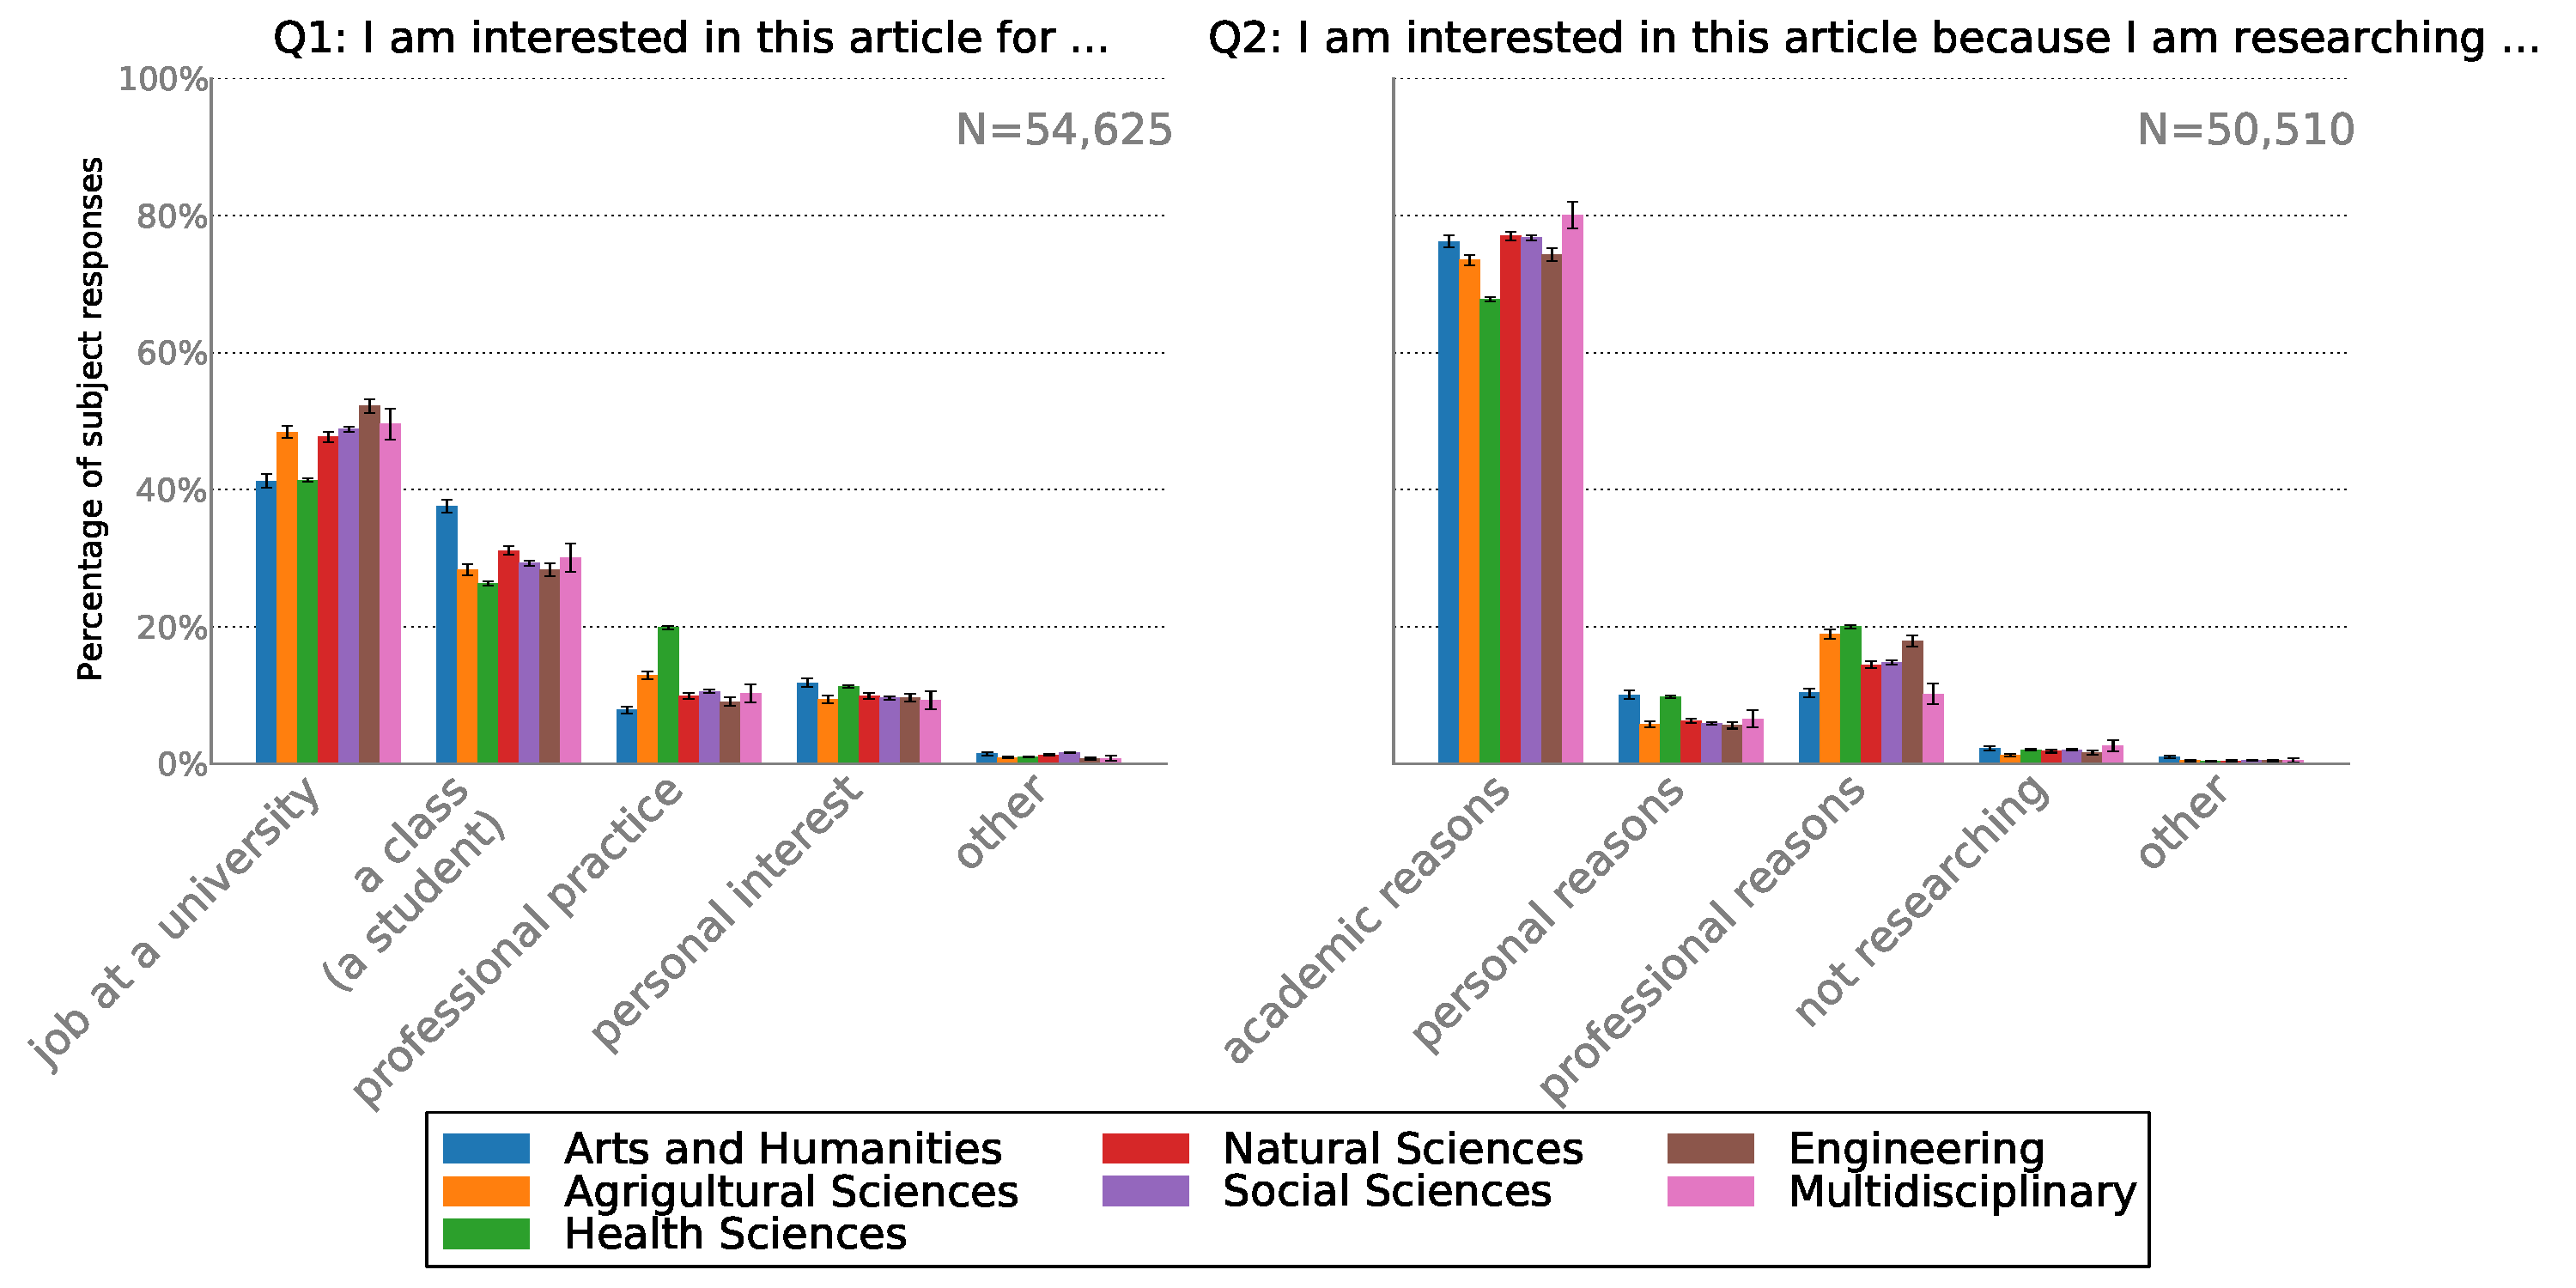
\includegraphics[keepaspectratio,width=\textwidth,height=0.75\textheight]{figures/scielo_q1_q2_by_latindex_subjects.pdf}
\caption{Responses to Q1 and Q2 by Subject (SciELO)}
\label{scielo_q1_q2_by_latindex_subjects}
\end{figure}

\begin{figure}[htbp]
\centering
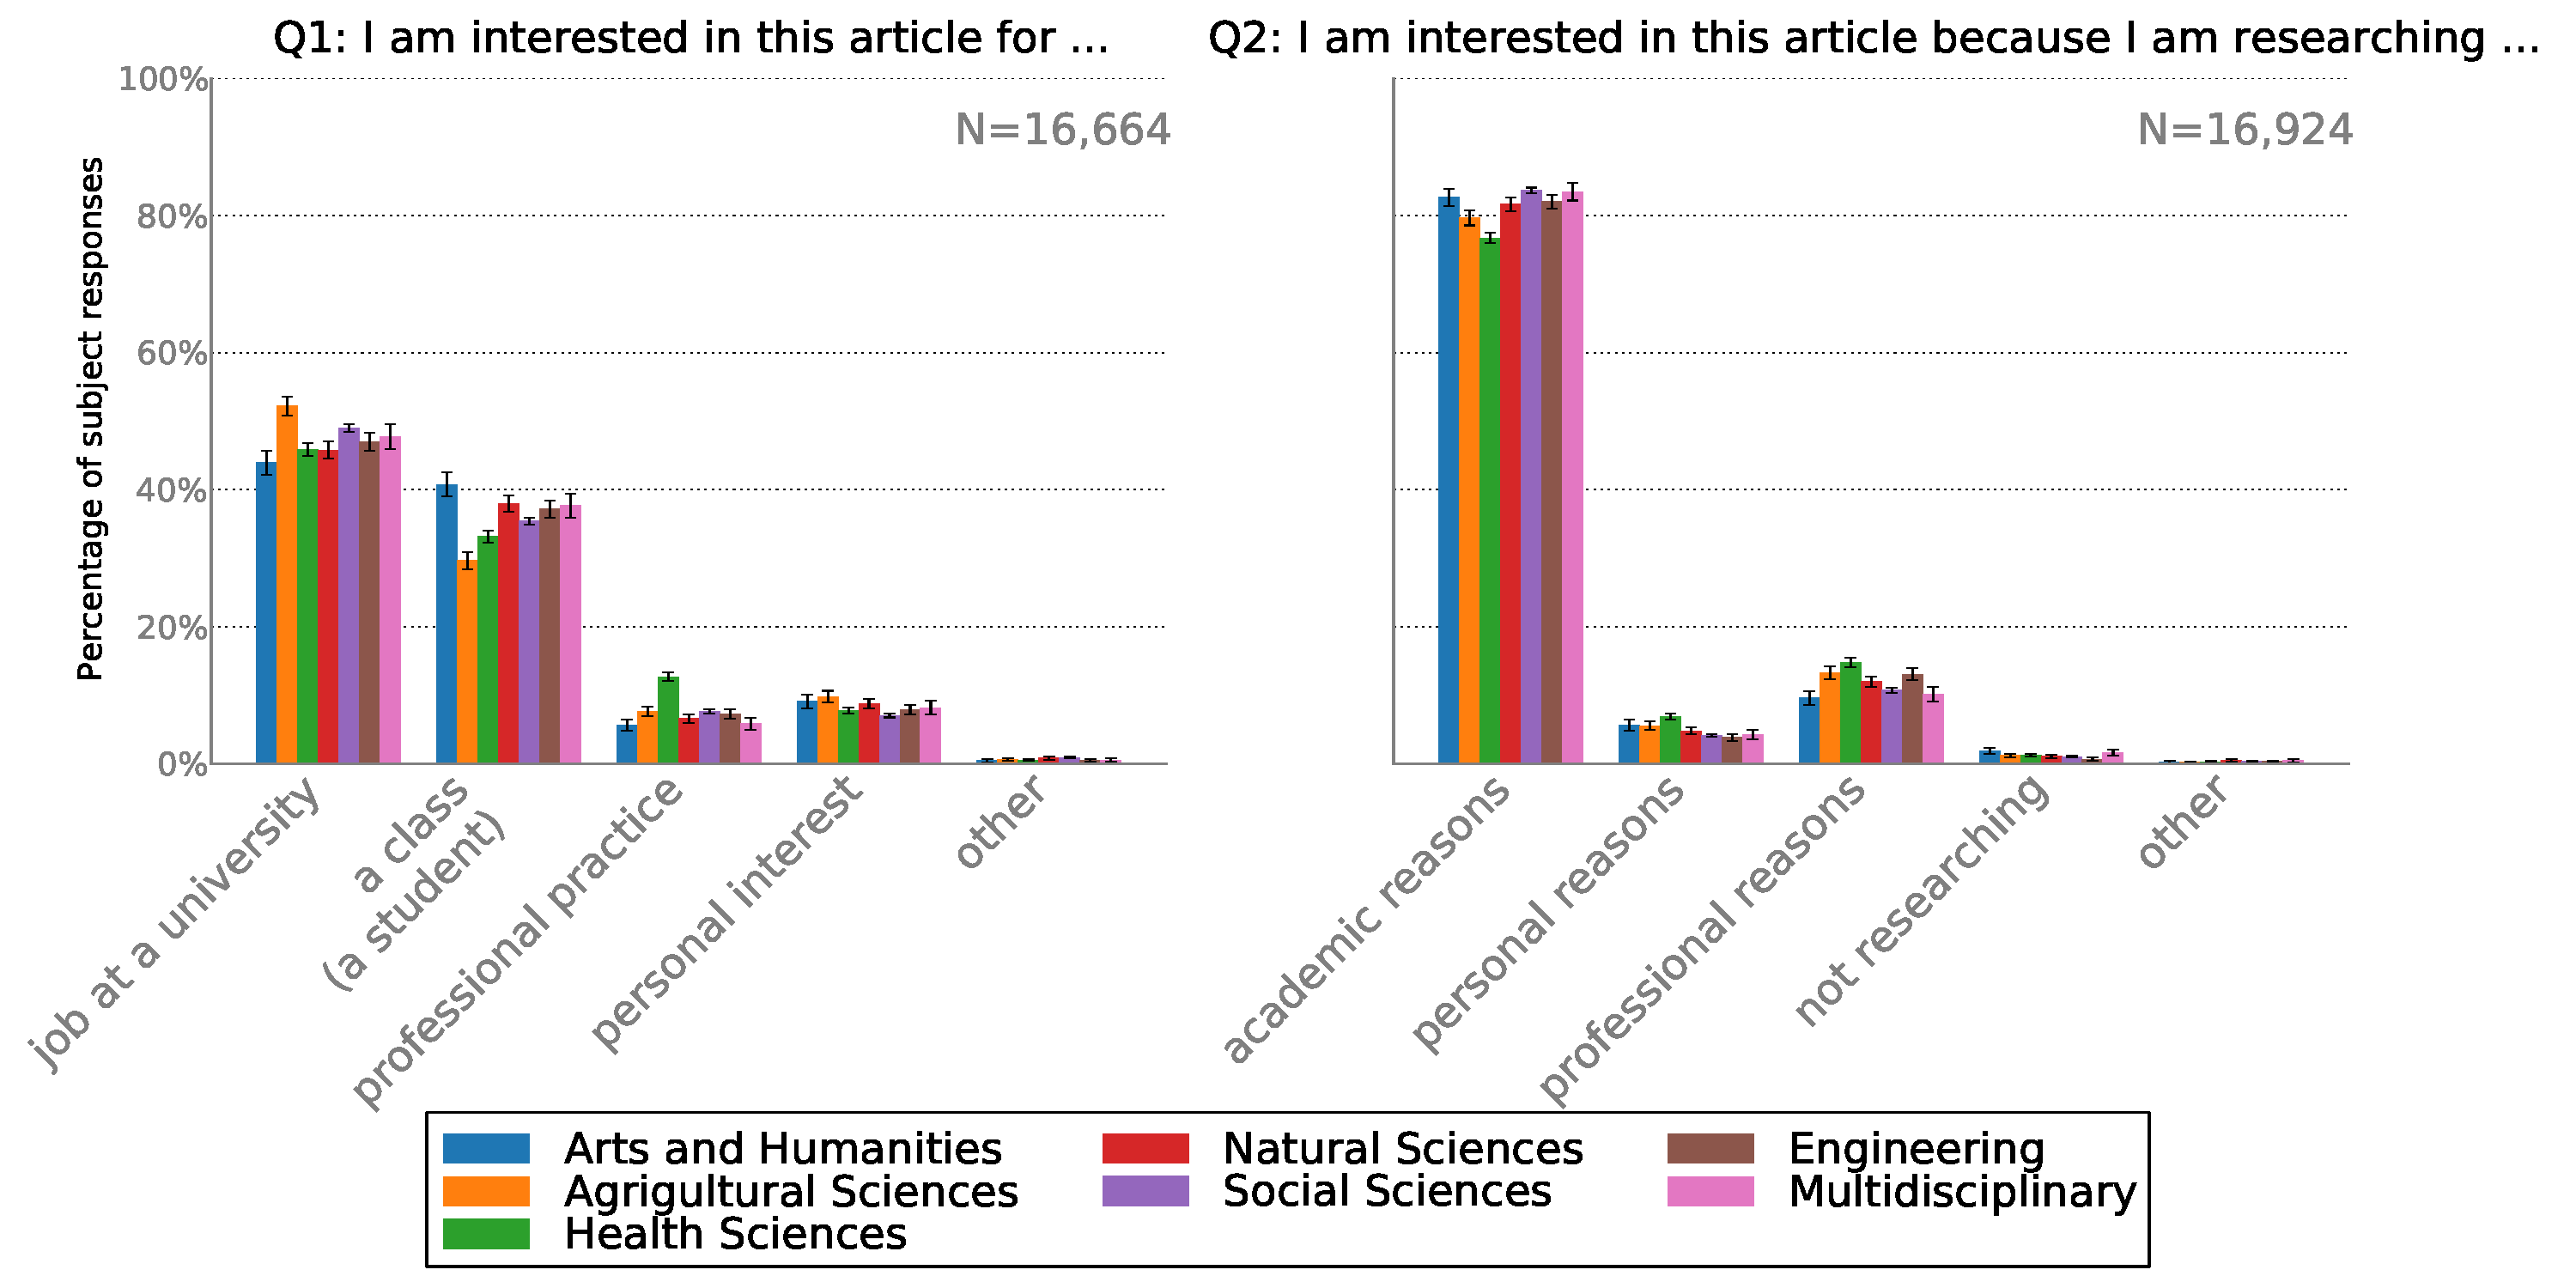
\includegraphics[keepaspectratio,width=\textwidth,height=0.75\textheight]{figures/redalyc_q1_q2_by_latindex_subjects.pdf}
\caption{Responses to Q1 and Q2 by Subject (RedALyC)}
\label{redalyc_q1_q2_by_latindex_subjects}
\end{figure}

\begin{figure}[htbp]
\centering
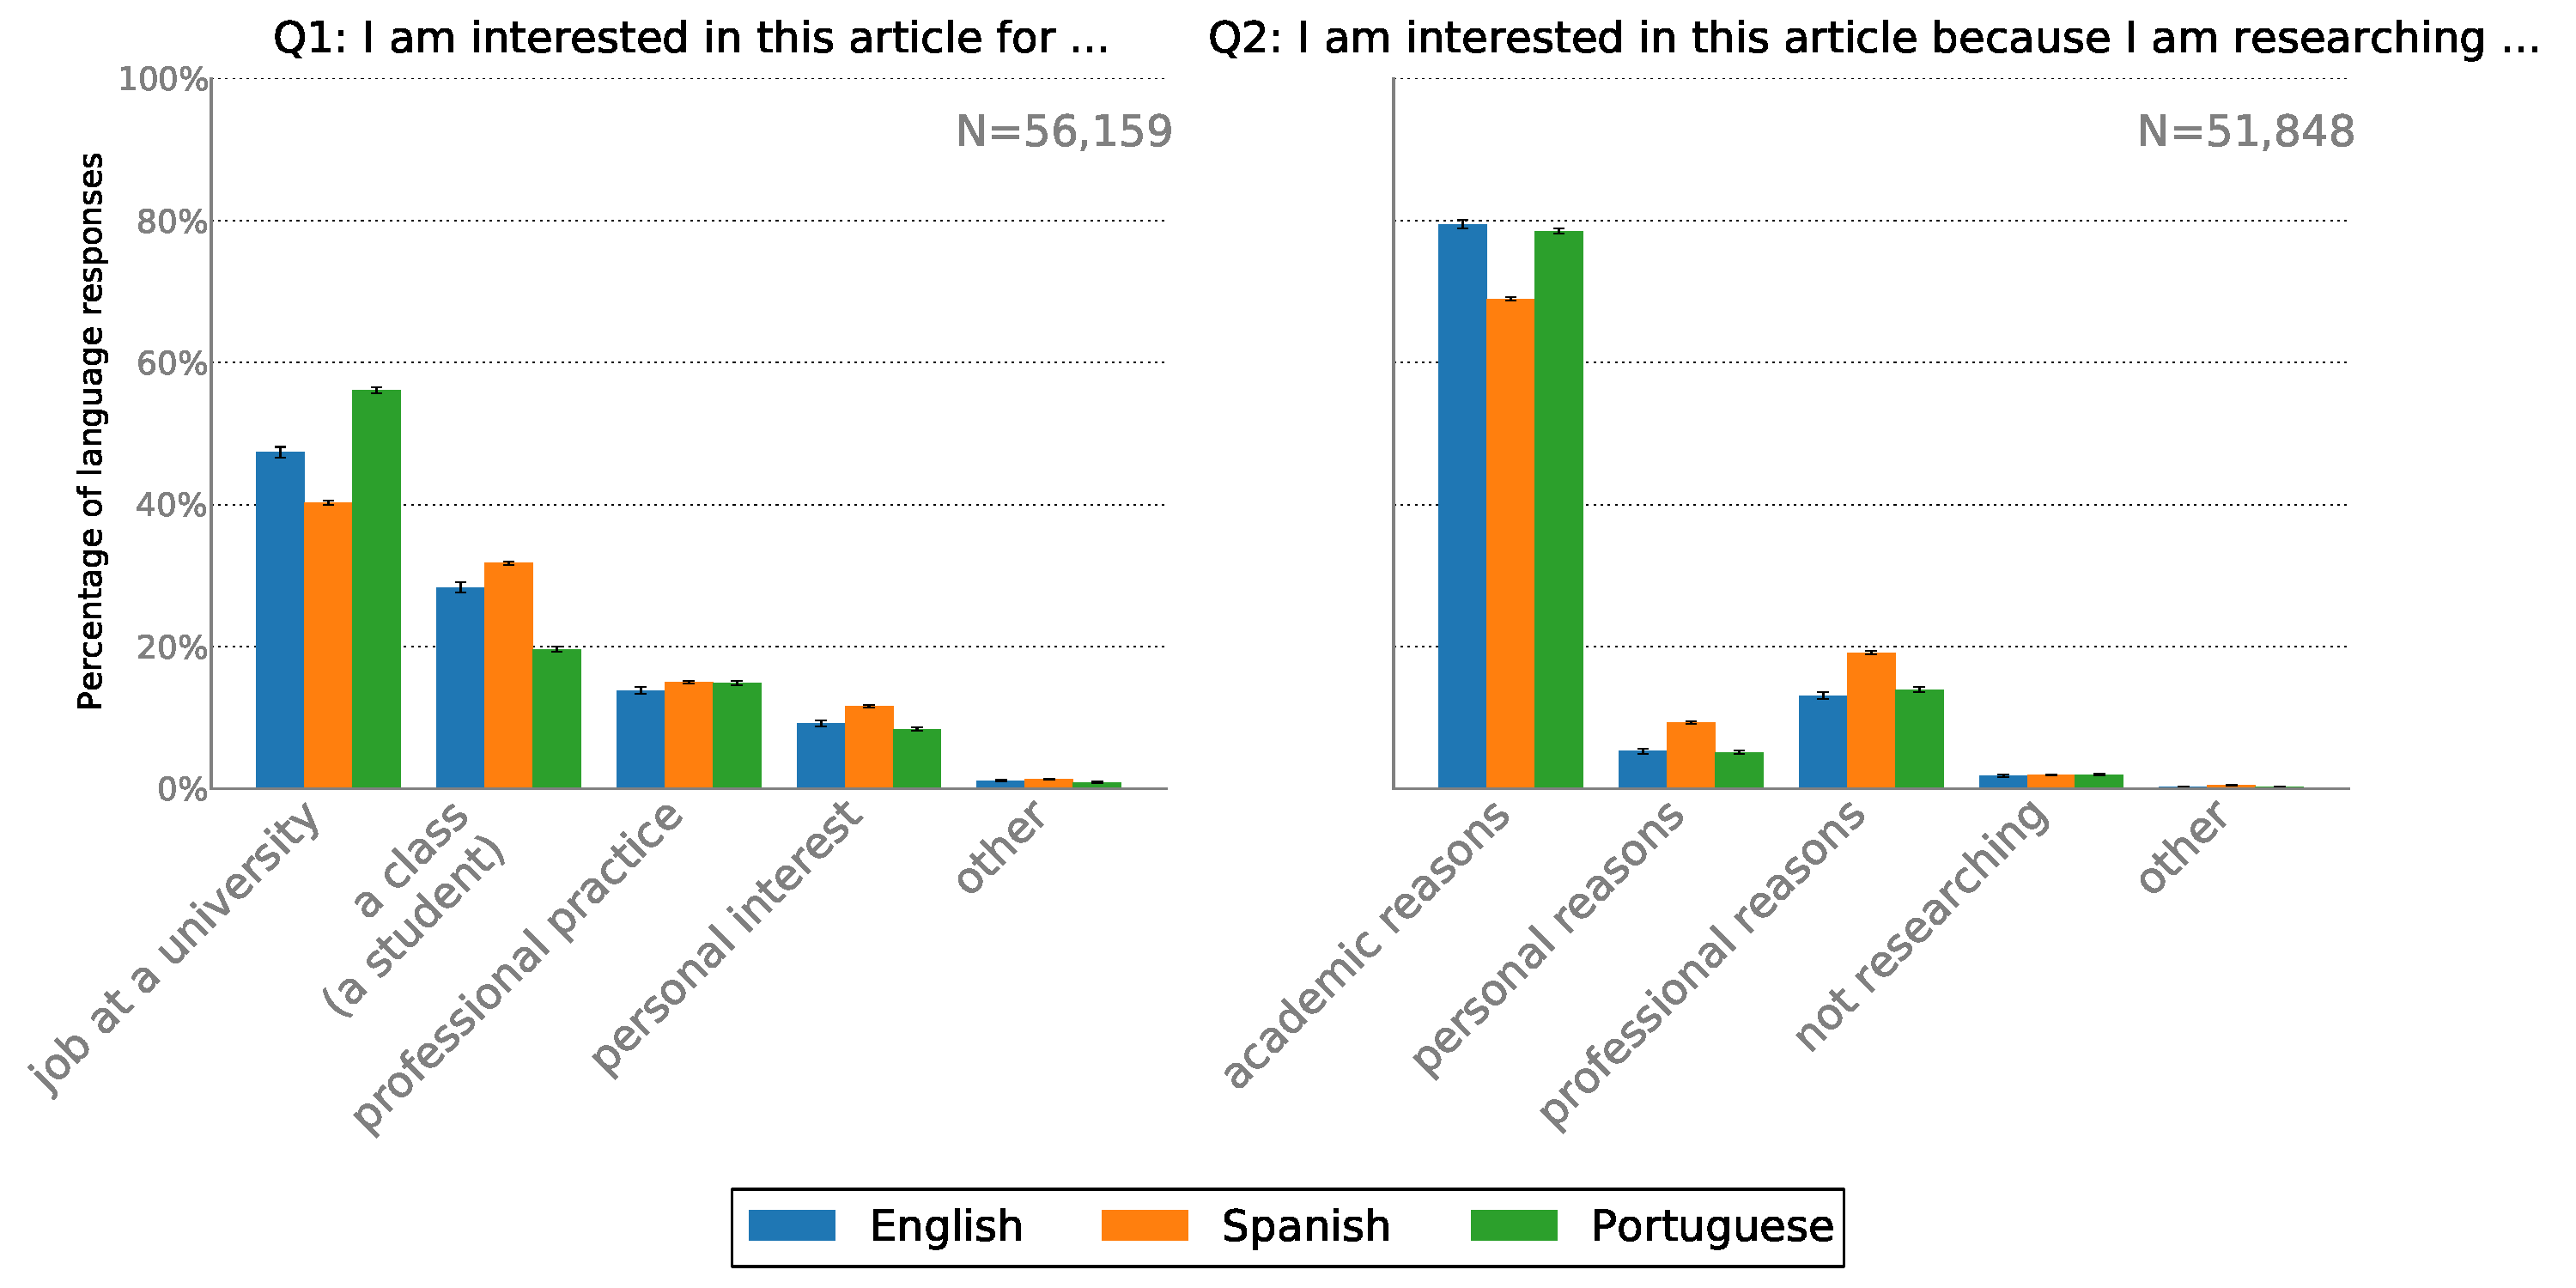
\includegraphics[keepaspectratio,width=\textwidth,height=0.75\textheight]{figures/scielo_q1_q2_by_original_language.pdf}
\caption{Responses to Q1 and Q2 by Language (SciELO)}
\label{scielo_q1_q2_by_original_language}
\end{figure}

\begin{figure}[htbp]
\centering
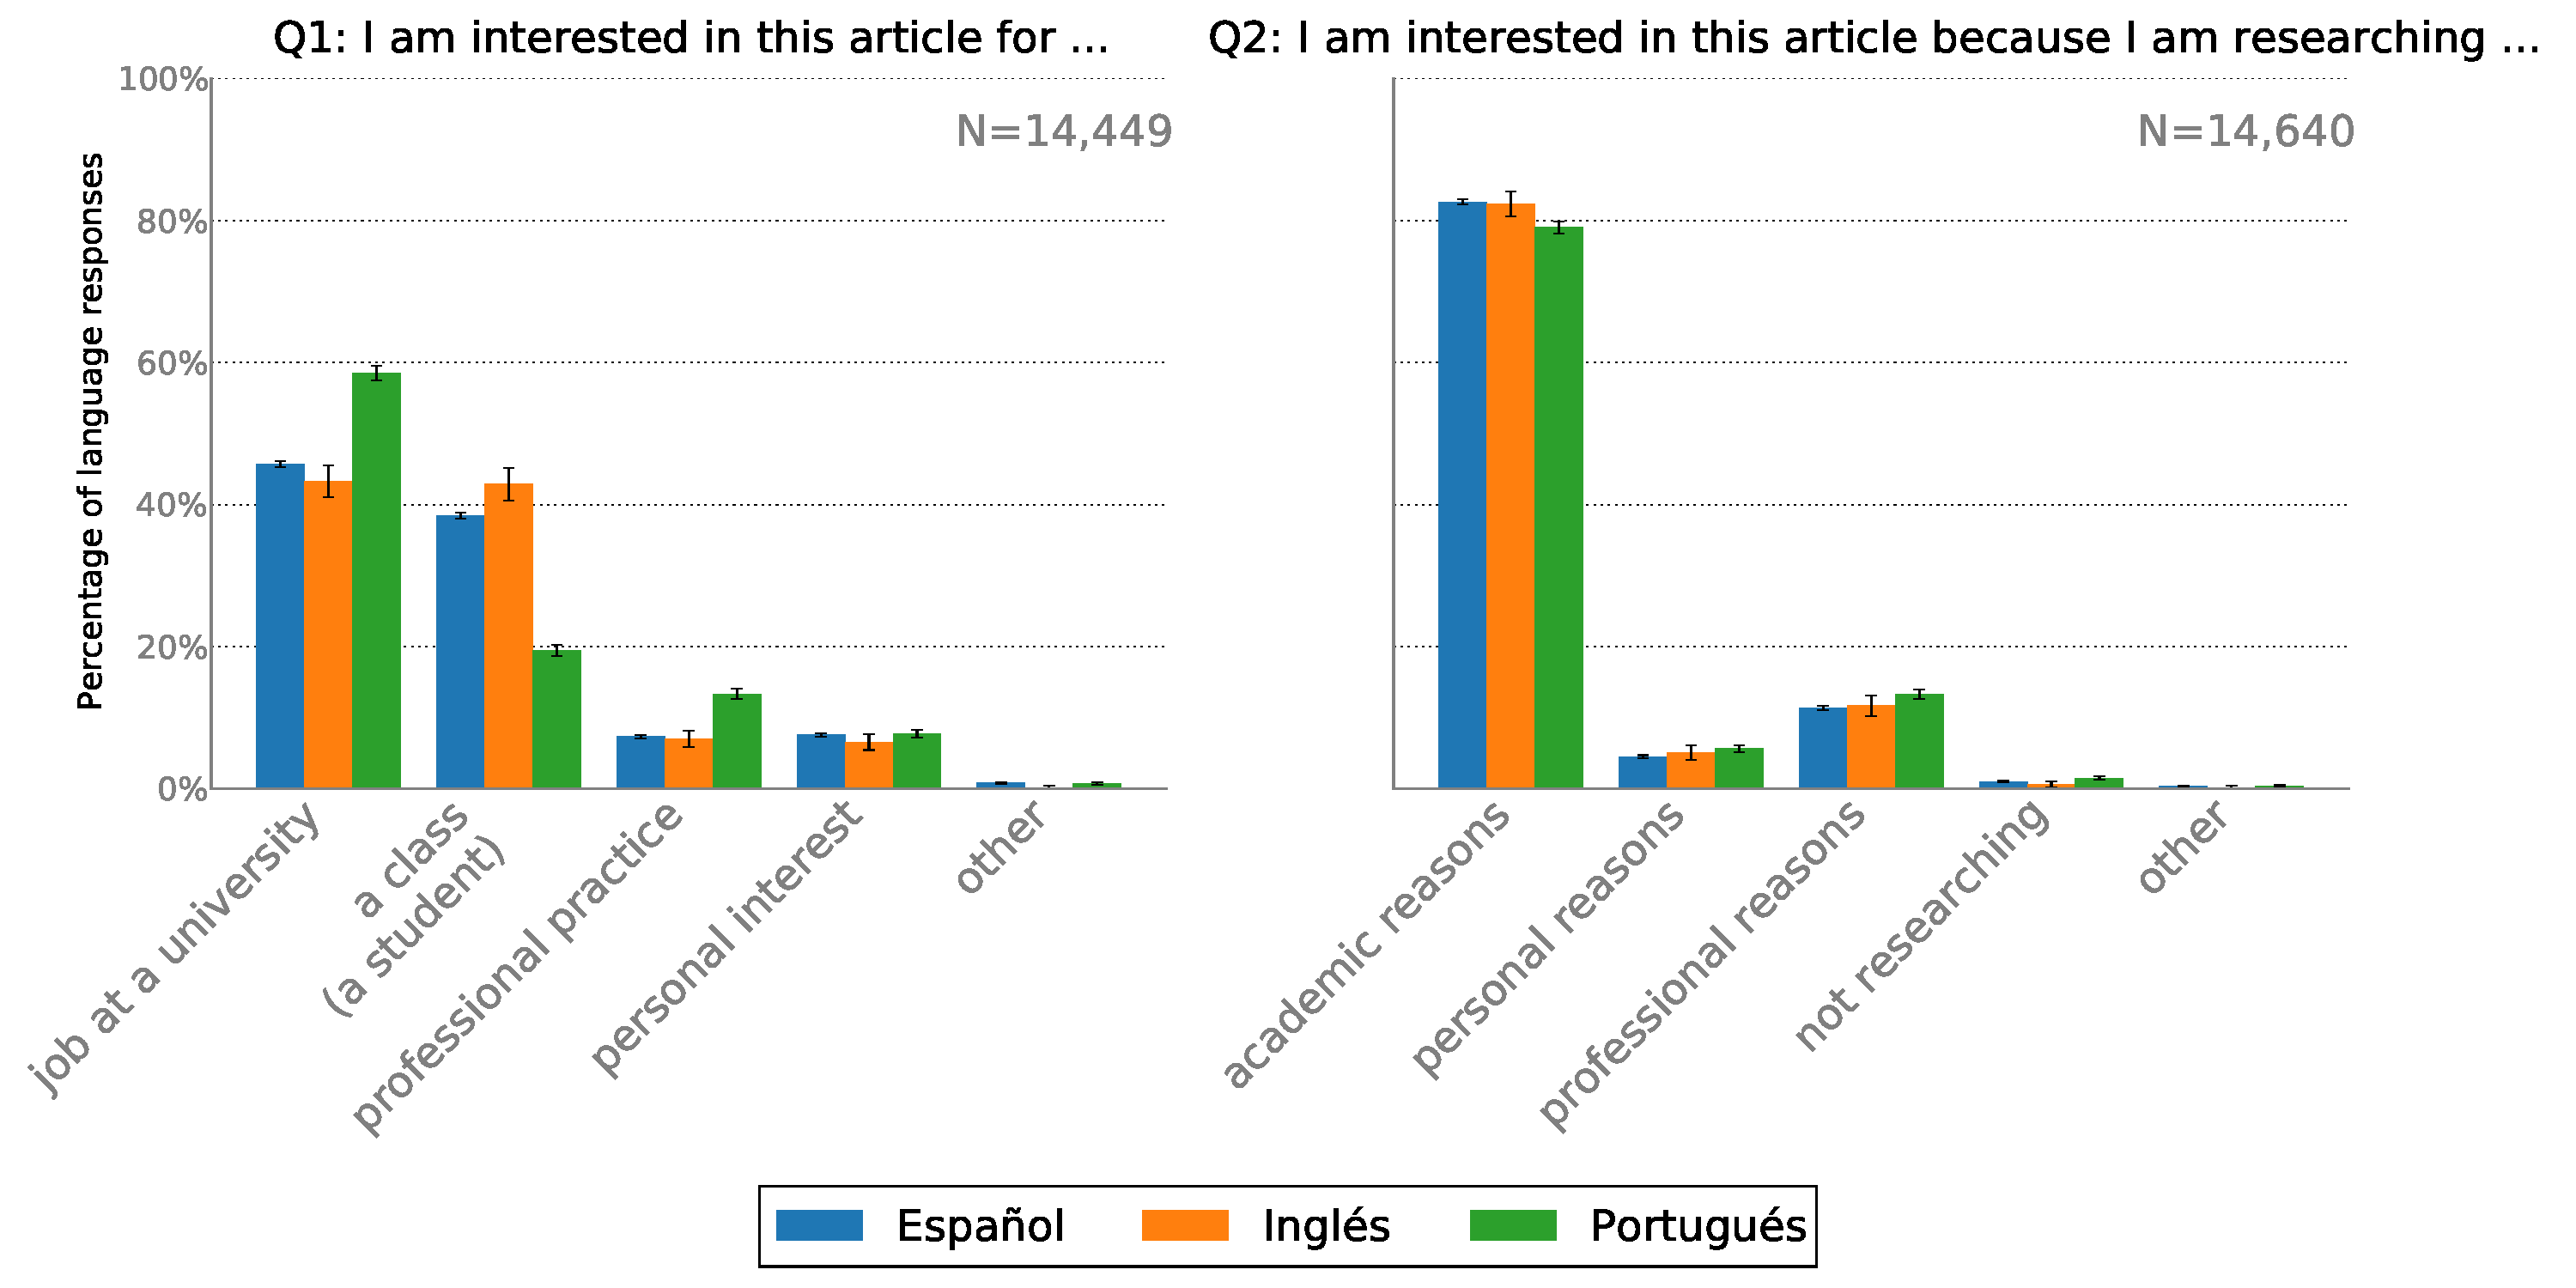
\includegraphics[keepaspectratio,width=\textwidth,height=0.75\textheight]{figures/redalyc_q1_q2_by_original_language.pdf}
\caption{Responses to Q1 and Q2 by Language (RedALyC)}
\label{redalyc_q1_q2_by_original_language}
\end{figure}

\begin{figure}[htbp]
\centering
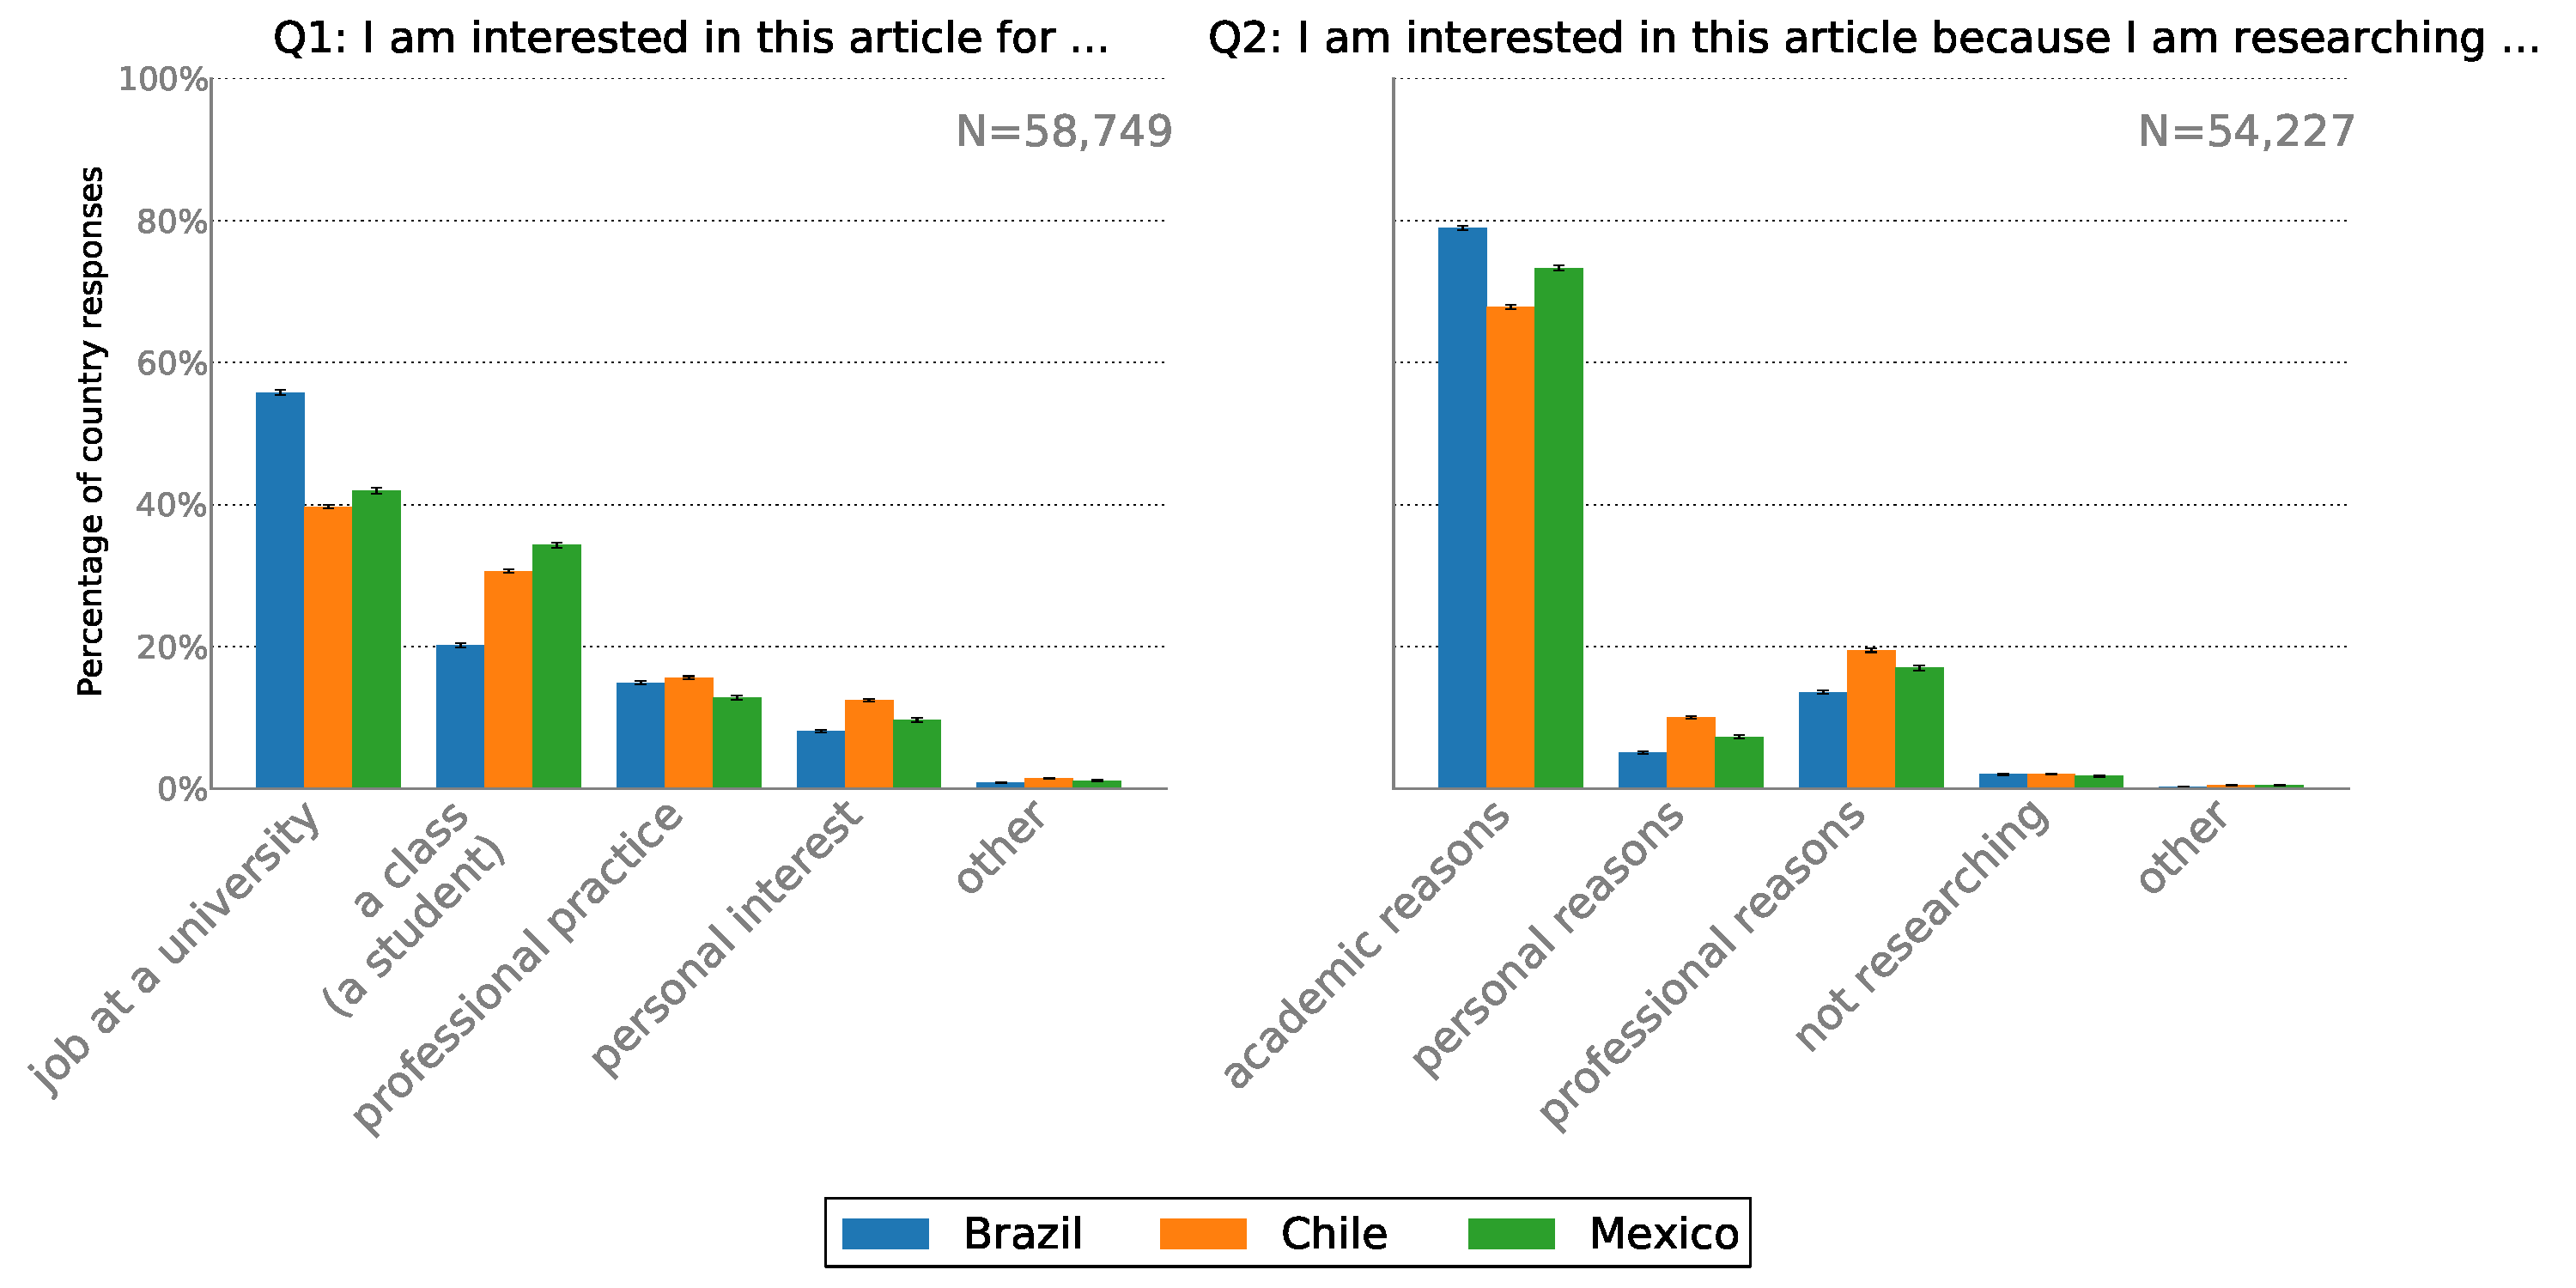
\includegraphics[keepaspectratio,width=\textwidth,height=0.75\textheight]{figures/scielo_q1_q2_by_country_journal.pdf}
\caption{Responses to Q1 and Q2 by Journal's Country (SciELO)}
\label{scielo_q1_q2_by_country_journal}
\end{figure}

\begin{figure}[htbp]
\centering
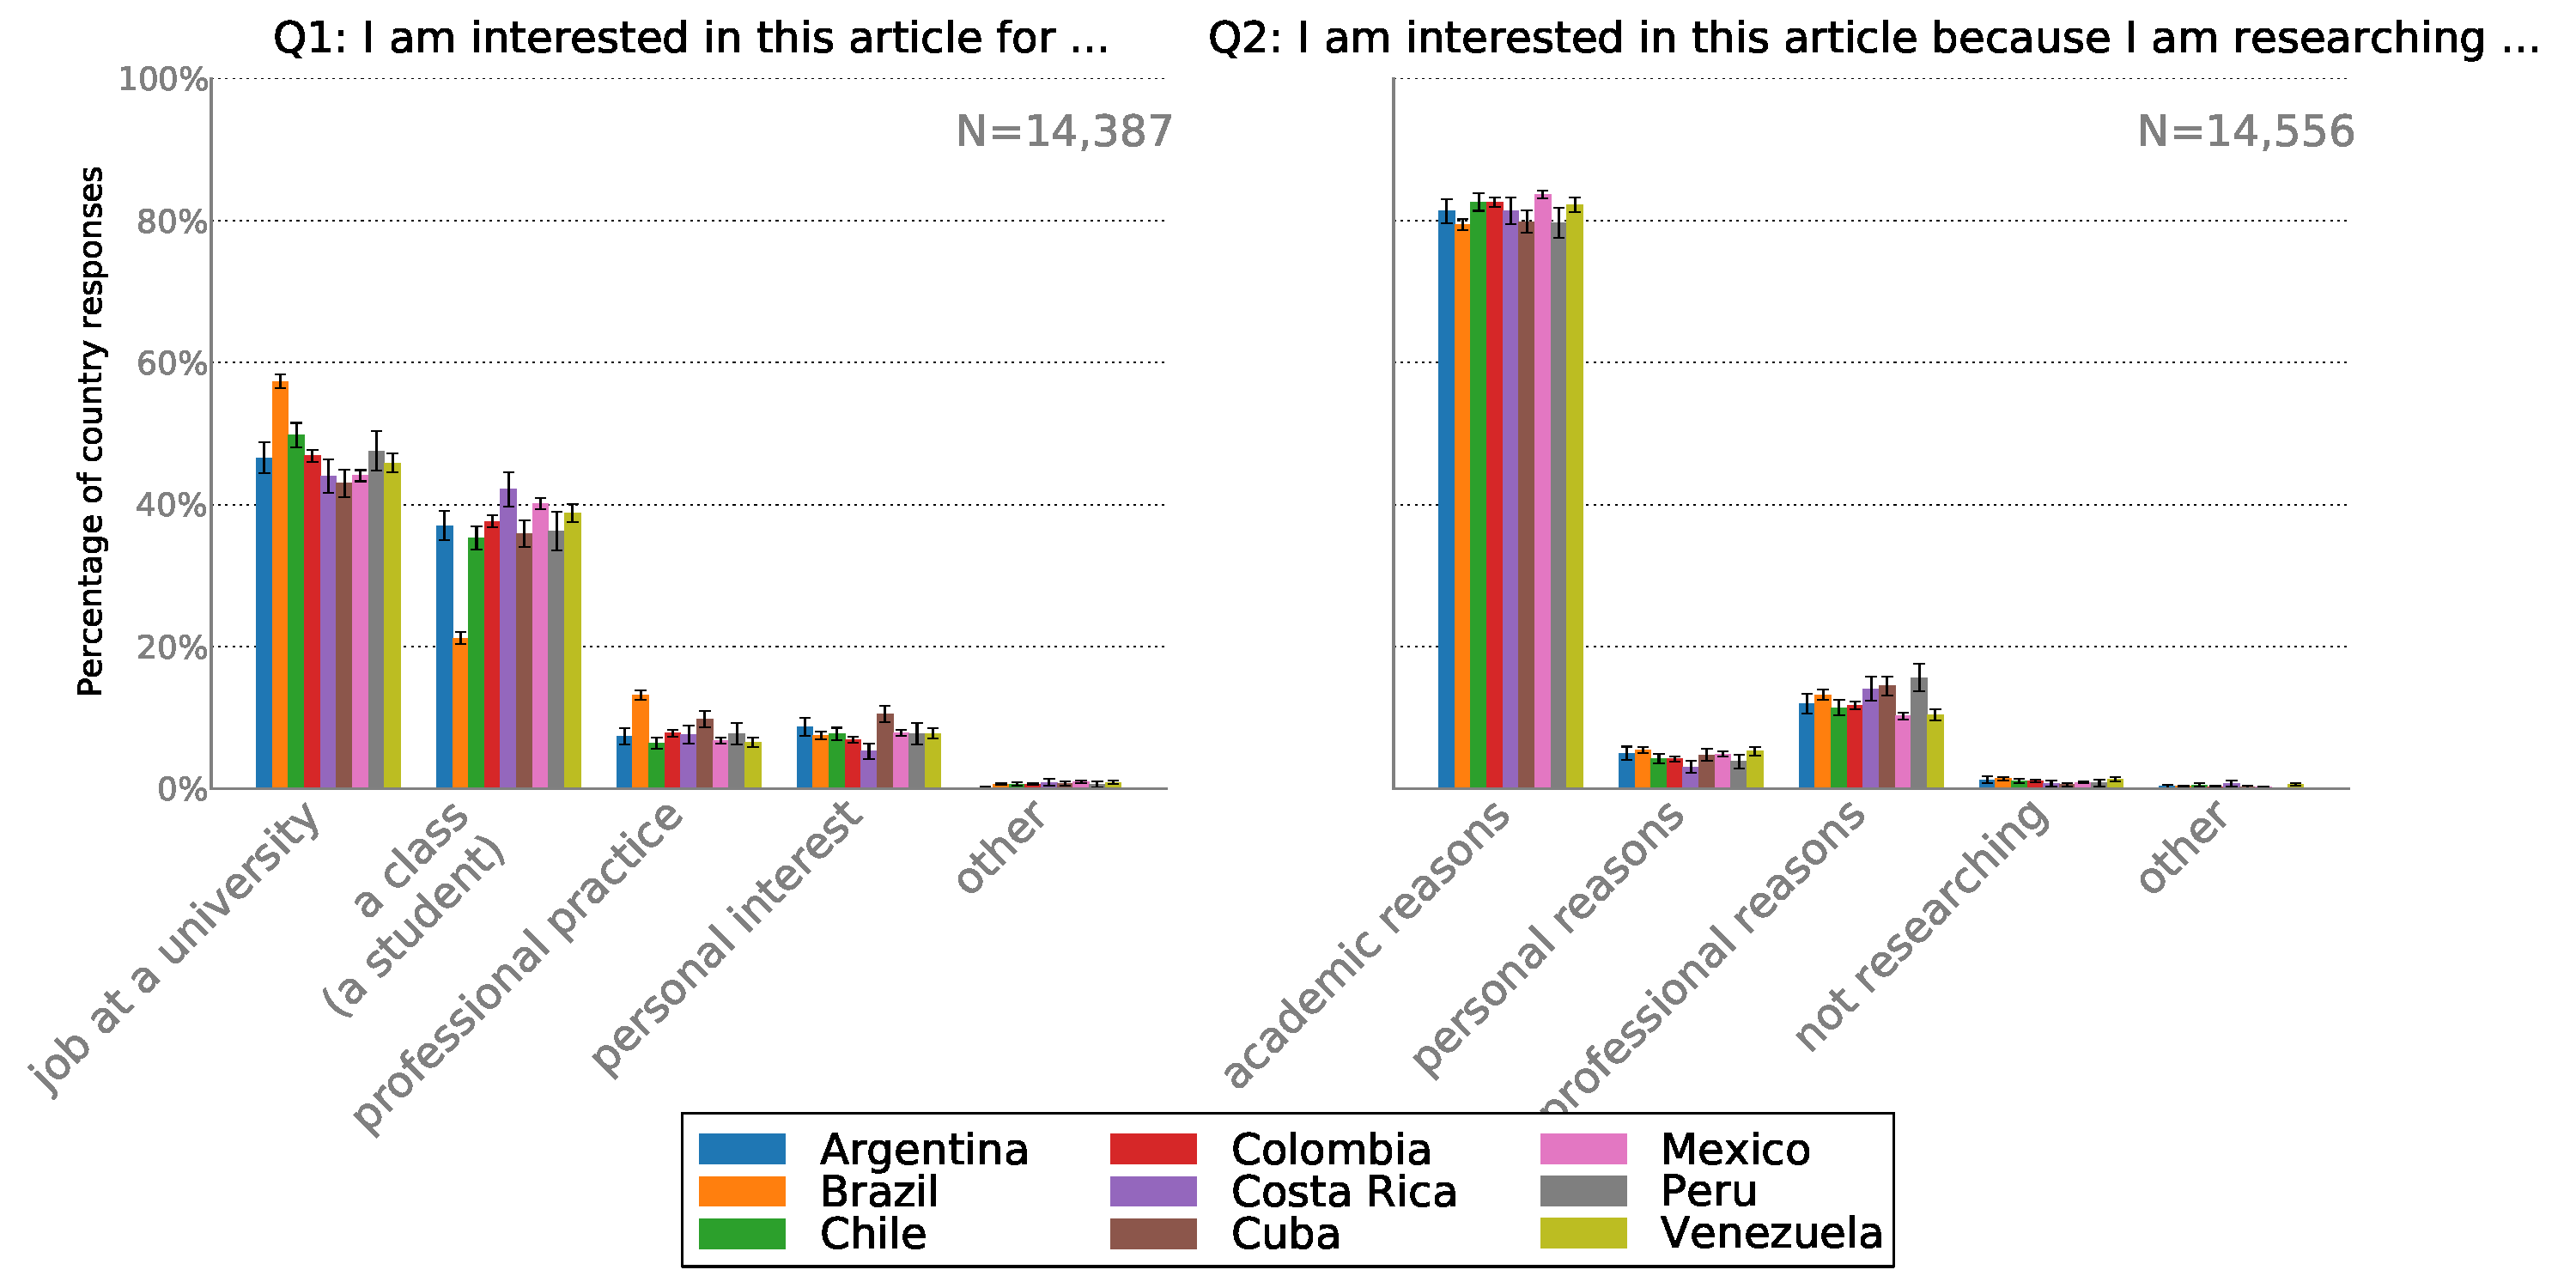
\includegraphics[keepaspectratio,width=\textwidth,height=0.75\textheight]{figures/redalyc_q1_q2_by_country_journal.pdf}
\caption{Responses to Q1 and Q2 by Journal's Country (RedALyC)}
\label{redalyc_q1_q2_by_country_journal}
\end{figure}

\subsection{Topics}
\label{topics}

The survey and pop-up results give a sense of the demographic that reads Latin American research, however, but only begins to give a sense on how this public changes based on the content of the articles. Of the breakdowns by subject field, language, and country of publication shown above, the disciplinary breakdown reveals a few areas that are consistent between the two portals. However, even this disciplinary breakdown is not entirely clear between the two portals, and the only persistent trend is the increased level of professional use among the respondents reading articles in medical science journals.

To better understand if the public and academic audiences are drawn to different subject matter it is necessary to look at the topics of the articles respondents were reading, not just the subjects of the journals. Labeled latent Dirichlet allocation (LLDA) topic models (described in the methods section above) are useful for understanding which terms are most prevalent for each of the responses. By building an LLDA model for each question, based on the titles of the papers that people were reading at the time of responding, we can compare the list of most salient terms for each response and quantify the similarities in the overall distributions of terms for each.

We can view two outputs that can help us understand the topics being read by each class of reader. First, we can simply look at the lists of top twenty terms found in each response according to the model. By looking within the terms associated with each response we can first get a sense of the topics of interest to each group. Then, by looking at the overlaps between groups we can begin to get a sense of which groups of readers are interested in the same content, something we can also do in more detail, by incorporating all terms.

If we look within group and across the sets of both portals, a few trends stand out. First, although we see health-related terms throughout all topics, they make the majority of the terms associated with public and non-profit sector respondents as well as that of those interested for personal reasons. Second, we see a series of research-related terms in the private sector respondents, such as ``research'' (pesquisa), ``revision'' + ``literatura'' (literature review), ``study'', and ``cases'' (casos). Finally, we see that the terms associated with both of the academic respondents are much more varied than others. While they include some youth-related terms, such as ``students'' (estudiantes), ``adolescents'' (adolescentes), ``children'' (niños), they also include a series of other terms ranging from ``environment'' (ambiental), to ``factors'' (factores), to ``nursing'' (enfermagem). The top--20 list of terms for each category of respondents can be found in \autoref{top20_terms_q1}.




\begin{longtable}{@{}lp{2.5cm}p{6.5cm}@{}}
\caption{Top 20 Terms in Topic Model of Q1 Responses}
\label{top20_terms_q1} \\
    \toprule
    \multicolumn{1}{l}{Response} & \multicolumn{1}{p{2.5cm}}{Portal} & \multicolumn{1}{p{6.5cm}}{Top 20 Terms in Model} \\
    \hline
\endfirsthead

\multicolumn{3}{c}%
{{\tablename\ \thetable{} -- continued from previous page}} \\
    \hline
    \multicolumn{1}{l}{Response} & \multicolumn{1}{p{2.5cm}}{Portal} & \multicolumn{1}{p{6.5cm}}{Top 20 Terms in Model} \\
    \hline
\endhead

\hline \multicolumn{3}{r}{{Continued on next page}} \\ \hline
\endfoot

\bottomrule
\endlastfoot
I am a Student  &   RedAlyC & estudiantes{\slash}relacion{\slash}adolescentes{\slash}sociales{\slash}ninos{\slash}uso{\slash}construccion{\slash}trabajo{\slash}hacia{\slash}ambiental{\slash}historia{\slash}factores{\slash}tratamiento{\slash}diseno{\slash}riesgo{\slash}sistemas{\slash}caracteristicas{\slash}teoria{\slash}perspectiva{\slash}universidad \\
    &   SciELO  &   salud{\slash}ciudad{\slash}desarrollo{\slash}ninos{\slash}adolescentes{\slash}factores{\slash}tratamiento{\slash}modelo{\slash}riesgo{\slash}educacion{\slash}prevalencia{\slash}region{\slash}anos{\slash}vida{\slash}relacion{\slash}estudiantes{\slash}hospital{\slash}sistema{\slash}clinico{\slash}efecto \\
    &   both    &   adolescentes{\slash}ninos{\slash}estudiantes{\slash}relacion{\slash}factores{\slash}tratamiento{\slash}riesgo \\ \hline
Work at a University    &   RedAlyC &   factores{\slash}gestion{\slash}brasil{\slash}uso{\slash}ninos{\slash}empresas{\slash}saude{\slash}pacientes{\slash}produccion{\slash}sistemas{\slash}vida{\slash}analise{\slash}enfermagem{\slash}avaliacao{\slash}sociales{\slash}teoria{\slash}aplicacion{\slash}tres{\slash}adolescentes{\slash}construccion \\
    &   SciELO  &   sistema{\slash}educacion{\slash}enfermagem{\slash}efecto{\slash}desarrollo{\slash}cancer{\slash}educacao{\slash}salud{\slash}politica{\slash}anos{\slash}modelo{\slash}tratamento{\slash}adolescentes{\slash}vida{\slash}diferentes{\slash}hospital{\slash}rio{\slash}programa{\slash}experiencia{\slash}trabalho \\
    &   both    &   enfermagem{\slash}vida{\slash}adolescentes \\ \hline
Work in Public Sector   &   RedALyC & enfermagem{\slash}pacientes{\slash}saude{\slash}culturas{\slash}tratamiento{\slash}clinica{\slash}hospital{\slash}docente{\slash}practica{\slash}terapia{\slash}revision{\slash}reporte{\slash}estimacion{\slash}politicas{\slash}competencias{\slash}publicas{\slash}renal{\slash}determinacion{\slash}base \\
    &   SciELO  &   tratamiento{\slash}casos{\slash}ninos{\slash}anos{\slash}experiencia{\slash}enfermedad{\slash}sindrome{\slash}cancer{\slash}clinico{\slash}manejo{\slash}prevalencia{\slash}revision{\slash}vida{\slash}paciente{\slash}literatura{\slash}impacto{\slash}factores{\slash}programa{\slash}aguda{\slash}nacional \\
    &   both    &   tratamiento{\slash}revision \\ \hline
Work in Private Sector  &   RedALyC &   pesquisa{\slash}valor{\slash}impacto{\slash}economico{\slash}pensamiento{\slash}organizaciones{\slash}espanol{\slash}indicadores{\slash}tratamiento{\slash}brasil{\slash}proceso{\slash}traves{\slash}experiencia{\slash}humano{\slash}generar{\slash}santander{\slash}pareja{\slash}sujeto{\slash}fraturas{\slash}perdon \\
    &   SciELO  &   diferentes{\slash}aspectos{\slash}sistema{\slash}pulmonar{\slash}enfermagem{\slash}casos{\slash}qualidade{\slash}efecto{\slash}adultos{\slash}revision{\slash}literatura{\slash}metodo{\slash}clinica{\slash}sindrome{\slash}revisao{\slash}test{\slash}cancer{\slash}corte{\slash}study{\slash}niveles \\
    &   both    &   - \\ \hline
Work in Non-Profit Sector   &   RedALyC &   pacientes{\slash}enfermagem{\slash}avaliacao{\slash}conocimiento{\slash}gestion{\slash}universidad{\slash}sistemas{\slash}renal{\slash}derechos{\slash}comunicacion{\slash}diagnostico{\slash}riesgo{\slash}factores{\slash}ninos{\slash}empresas{\slash}familiar{\slash}analise{\slash}clinico{\slash}proposta{\slash}vida \\
    &   SciELO  &   tratamento{\slash}ninos{\slash}tratamiento{\slash}adolescentes{\slash}infeccion{\slash}anos{\slash}diabetes{\slash}central{\slash}clinico{\slash}edad{\slash}cancer{\slash}revision{\slash}tipo{\slash}literatura{\slash}resultados{\slash}sistema{\slash}prevencion{\slash}casos{\slash}sindrome{\slash}qualidade \\
    &   both    &   ninos{\slash}clinico \\ \hline
Personal Interest   &   RedALyC &   diferentes{\slash}produccion{\slash}economia{\slash}gestion{\slash}caracteristicas{\slash}publicas{\slash}superior{\slash}rendimiento{\slash}partir{\slash}aprendizaje{\slash}estrategias{\slash}prevalencia{\slash}aplicacion{\slash}relacion{\slash}crecimiento{\slash}reflexiones{\slash}argentina{\slash}nacional{\slash}ninos{\slash}universitaria \\
    &   SciELO  &   tratamiento{\slash}tratamento{\slash}literatura{\slash}manejo{\slash}casos{\slash}enfermedad{\slash}sindrome{\slash}anos{\slash}experiencia{\slash}revision{\slash}clinico{\slash}clinica{\slash}factores{\slash}desarrollo{\slash}control{\slash}region{\slash}relacion{\slash}historia{\slash}ninos{\slash}prevalencia \\
    &   both    &   relacion{\slash}prevalencia{\slash}ninos \\
\end{longtable}


The top--20 words for each group of respondents serves as a summary of the model and provides a qualitative sense of what each group is primarily interested in. However, it is a limited way of understanding the degree of similarities between groups. For a more quantitative measure, we calculate the cosine similarity score using the term-distribution vectors for each of the groups. That is, for each group, we look at the the model's loading of each term (the distribution) and construct a matrix where each row is a group (topic), each column is one of the 5,998 terms in the RedALyC or 14,924 terms in the SciELO corpuses, and the cells corresponding to the ``load'' of that term for that group. Each row in that matrix constitutes a vector and the angular distance between those vectors is calculated. In cosine similarity, 0 indicates the two vectors are ``pointing'' in the same direction (i.e., the same distribution of terms) and 1 indicates that the two vectors are orthogonal (i.e., the exact opposite distribution of terms).

We construct a symmetric matrix, where each of the groups are repeated along the rows and columns and with cell \emph{i,j} containing the cosine similarity score between the two term distribution vectors of groups \emph{i} and \emph{j}. As can be seen in \autoref{llda_cosine_similarity_q1}, the two most similar term distribution vectors are between the terms associated with ``I am a student'' and ``my work at a university'', indicating that there is very little difference between the topics being read by students and others that fall under the academic category. In fact, the ``my work at a university'' category is the most similar to all others, probably indicating that the topics read by academics generally is diverse enough that it covers the same topics being read by all other groups (and especially students).

\begin{figure}[htbp]
\centering
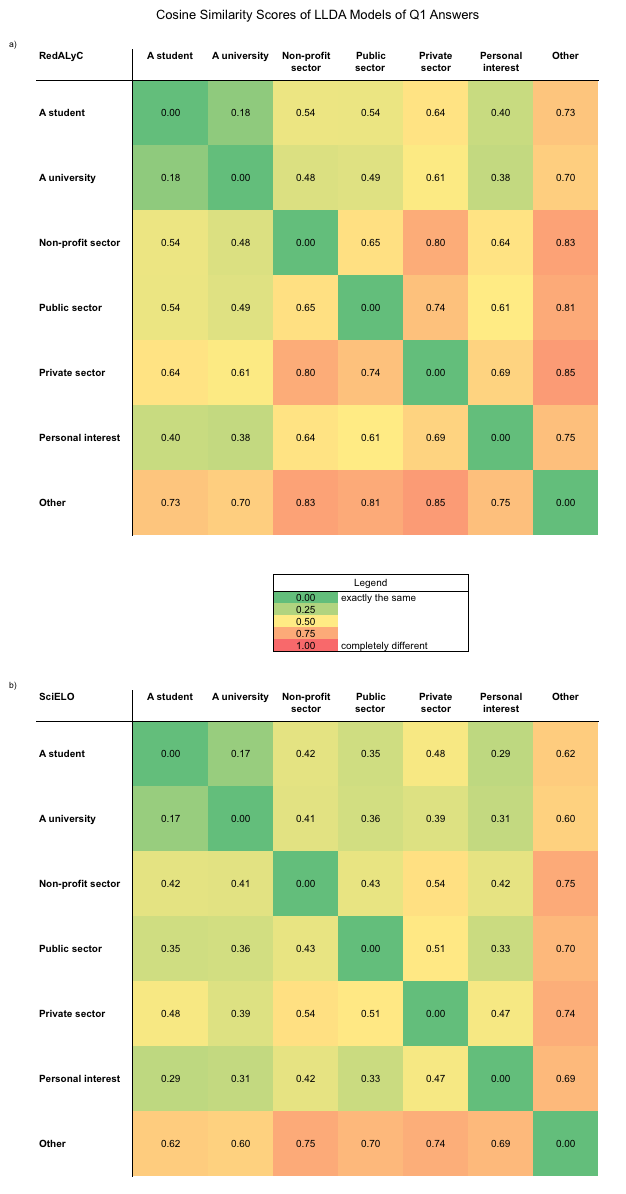
\includegraphics[keepaspectratio,width=\textwidth,height=0.95\textheight]{figures/llda_cosine_similarity_q1.png}
\caption{Cosine Similarity of LLDA Models of Q1 Responses}
\label{llda_cosine_similarity_q1}
\end{figure}

In contrast, the private sector readers appear to be the ones who read topics that set them further apart from the other groups.\footnote{Other than the ``other'' category, which is made up of terms for very few and disperate documents and is therefore omitted from the subsequent analysis.} The two most dissimilar term distributions, in both portals, are between those from the documents read by private and non-profit sector readers, followed closely by private and public sector readers. We actually see a strong similarity between the overall rankings of similarities between the two portals even though the cosine scores in the SciELO portals are generally lower than those in the RedALyC portal. Both rankings place the private sector readers as accessing the most dissimilar content to other groups, followed by the non-profit and public sectors, those reading for personal interest, students, and finally academics.

The corresponding matrix can be constructed for the responses from Q2 which has less detailed categories, and we see similar, but not entirely analogous results. In this case, the topics of those researching for personal reasons appear to be more dissimilar from the others than the topics of those researching for professional reasons.

\begin{figure}[htbp]
\centering
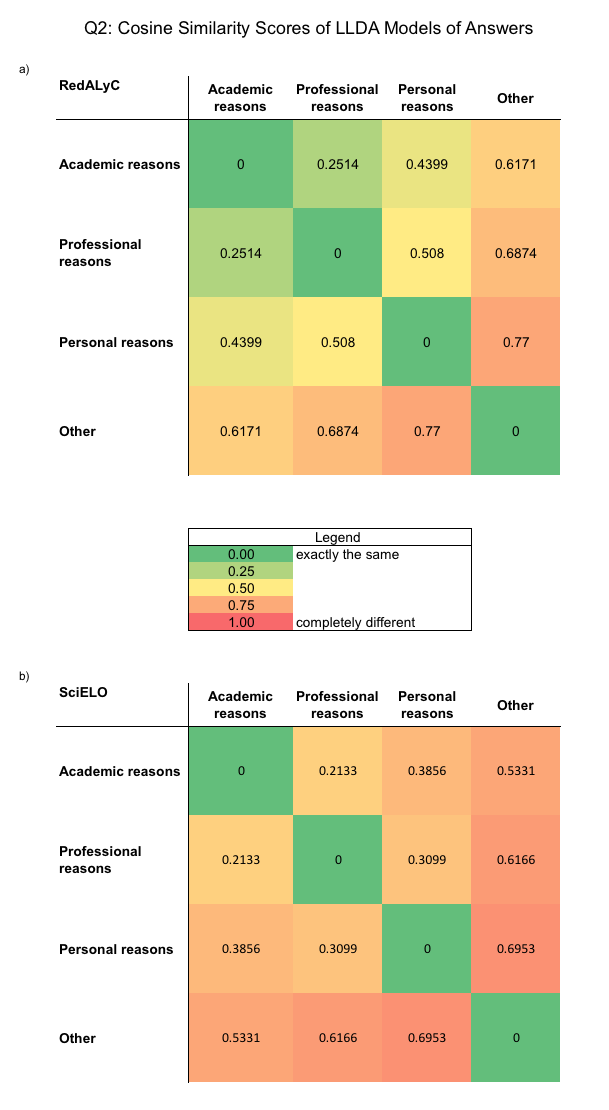
\includegraphics[keepaspectratio,width=\textwidth,height=0.95\textheight]{figures/llda_cosine_similarity_q2.png}
\caption{Cosine Similarity of LLDA Models of Q2 Responses}
\label{llda_cosine_similarity_q2}
\end{figure}

Overall, the topic models for both portals suggest that those researching for each of the two academic reasons are interested in more similar topics than those researching for any of the three professional reasons. It also suggests that all readers researching for professional reasons have a unique topic profile, but that those researching from the private sector are especially different from the rest. These differences hold despite the presence of health-related terms throughout noted above, with the notable exception of the SciELO portal's public sector and personal categories. These two are actually quite similar to each other (cosine score of .332), indicating that the SciELO portal is serving as a medical library for those coming for personal reasons more so than the RedALyC portal.

\subsection{Extent}
\label{extent}

While the surveys provide a sense of the demographics of users and the topic models an indication of the content that is accessed by the various groups, neither of these give us a sense of the scale of usage. Just as the topic models provide a deeper understanding of the how usage breaks down by content, a look at the number of downloads that articles receive can contextualize the degree of interest received, thereby giving us a sense of scale.

Ideally, downloads would be studied using a download window that took into account the usage half-life of articles. However, given that usage half-lives tend to be longer than 36 months ~\citep{Davis2013}, and we only have 12 months of data available, we must restrict our analysis to shorter time windows. To provide a sense of scale, we can look at the longest possible time period available, 12 months (all of 2013), by looking at the total download counts for articles that went online in January 2013. For those article, the mean number of total downloads between publication and the end of the year was 166 (st. dev. 229, N=699) in RedALyC and 778 (st. dev. 569, N=2,557) in SciELO.

For a more complete analysis, we can shorten the time window to either the first 30 or 90 days since being posted online (this only removes articles published after December 1st or October 2nd from the dataset). In the RedALyC portal, the mean number of downloads in the first 30 days since an article is posted online is 11 (st. dev. 16, N=30,897), and in the first 90 days it is 32 (st. dev. 48, N=26,810). In the SciELO portal, these numbers are several times higher, with 96 (st. dev. 206, N=20,077) and 241 (st. dev. 288, N=18,318) in the first 30 and 90 days respectively.

As expected, the Spearman's rank correlation between the 30 and 90 day download counts is a fairly high in both portals (0.70 in RedALyC and 0.92 in SciELO) and, as a result, the analysis using either set yields almost identical results. In the interest of capturing as large a window as possible to account for different speeds of uptake across fields, the subsequent analysis uses a 90 day window, and therefore includes all articles published between January 1st, and October 2nd, 2013.

Both portals show some differences between disciplines, with a mean number of downloads ranging between 178 and 284 in SciELO (\autoref{downloads90_by_subject_scielo}) and 26 and 54 in RedALyC (\autoref{downloads90_by_subject_redalyc}). The relative strength of SciELO's medical sciences (where SciELO has it's origins) can be seen by the boxplot, where the mean number of downloads surpases the 75th percentile of all the other subject fields (\autoref{downloads90_by_subject_scielo}). The same is true for the multidisciplinary journals in RedALyC, although in that case the N is significantly small (only 973 articles) (\autoref{downloads90_by_subject_redalyc}). A comparison of the median values, however, shows a less pronounced cross-disciplinary effect.

A between-country analysis is not possible for SciELO because the download data is only available for Brazil, but in the RedALyC journals we see that mean downloads range between 19 (Brazil) and 50 (Mexico). This may be indicative of the Spanish language bias of RedALyC users (who may be less likely to read articles from Brazil, which are largely in Portuguese) and of a local bias because of greater awareness of RedALyC in Mexico (Bongiovani et al., forthcoming). The boxplot depicted in \autoref{downloads90_by_country_redalyc} shows the differences between countries do exist, although they largely do not appear to be significant.\footnote{The y-axis of the box plots are cut off arbitrarily (hiding outliers) for the sake of clarity near the x-axis.}

\begin{figure}[htbp]
\centering
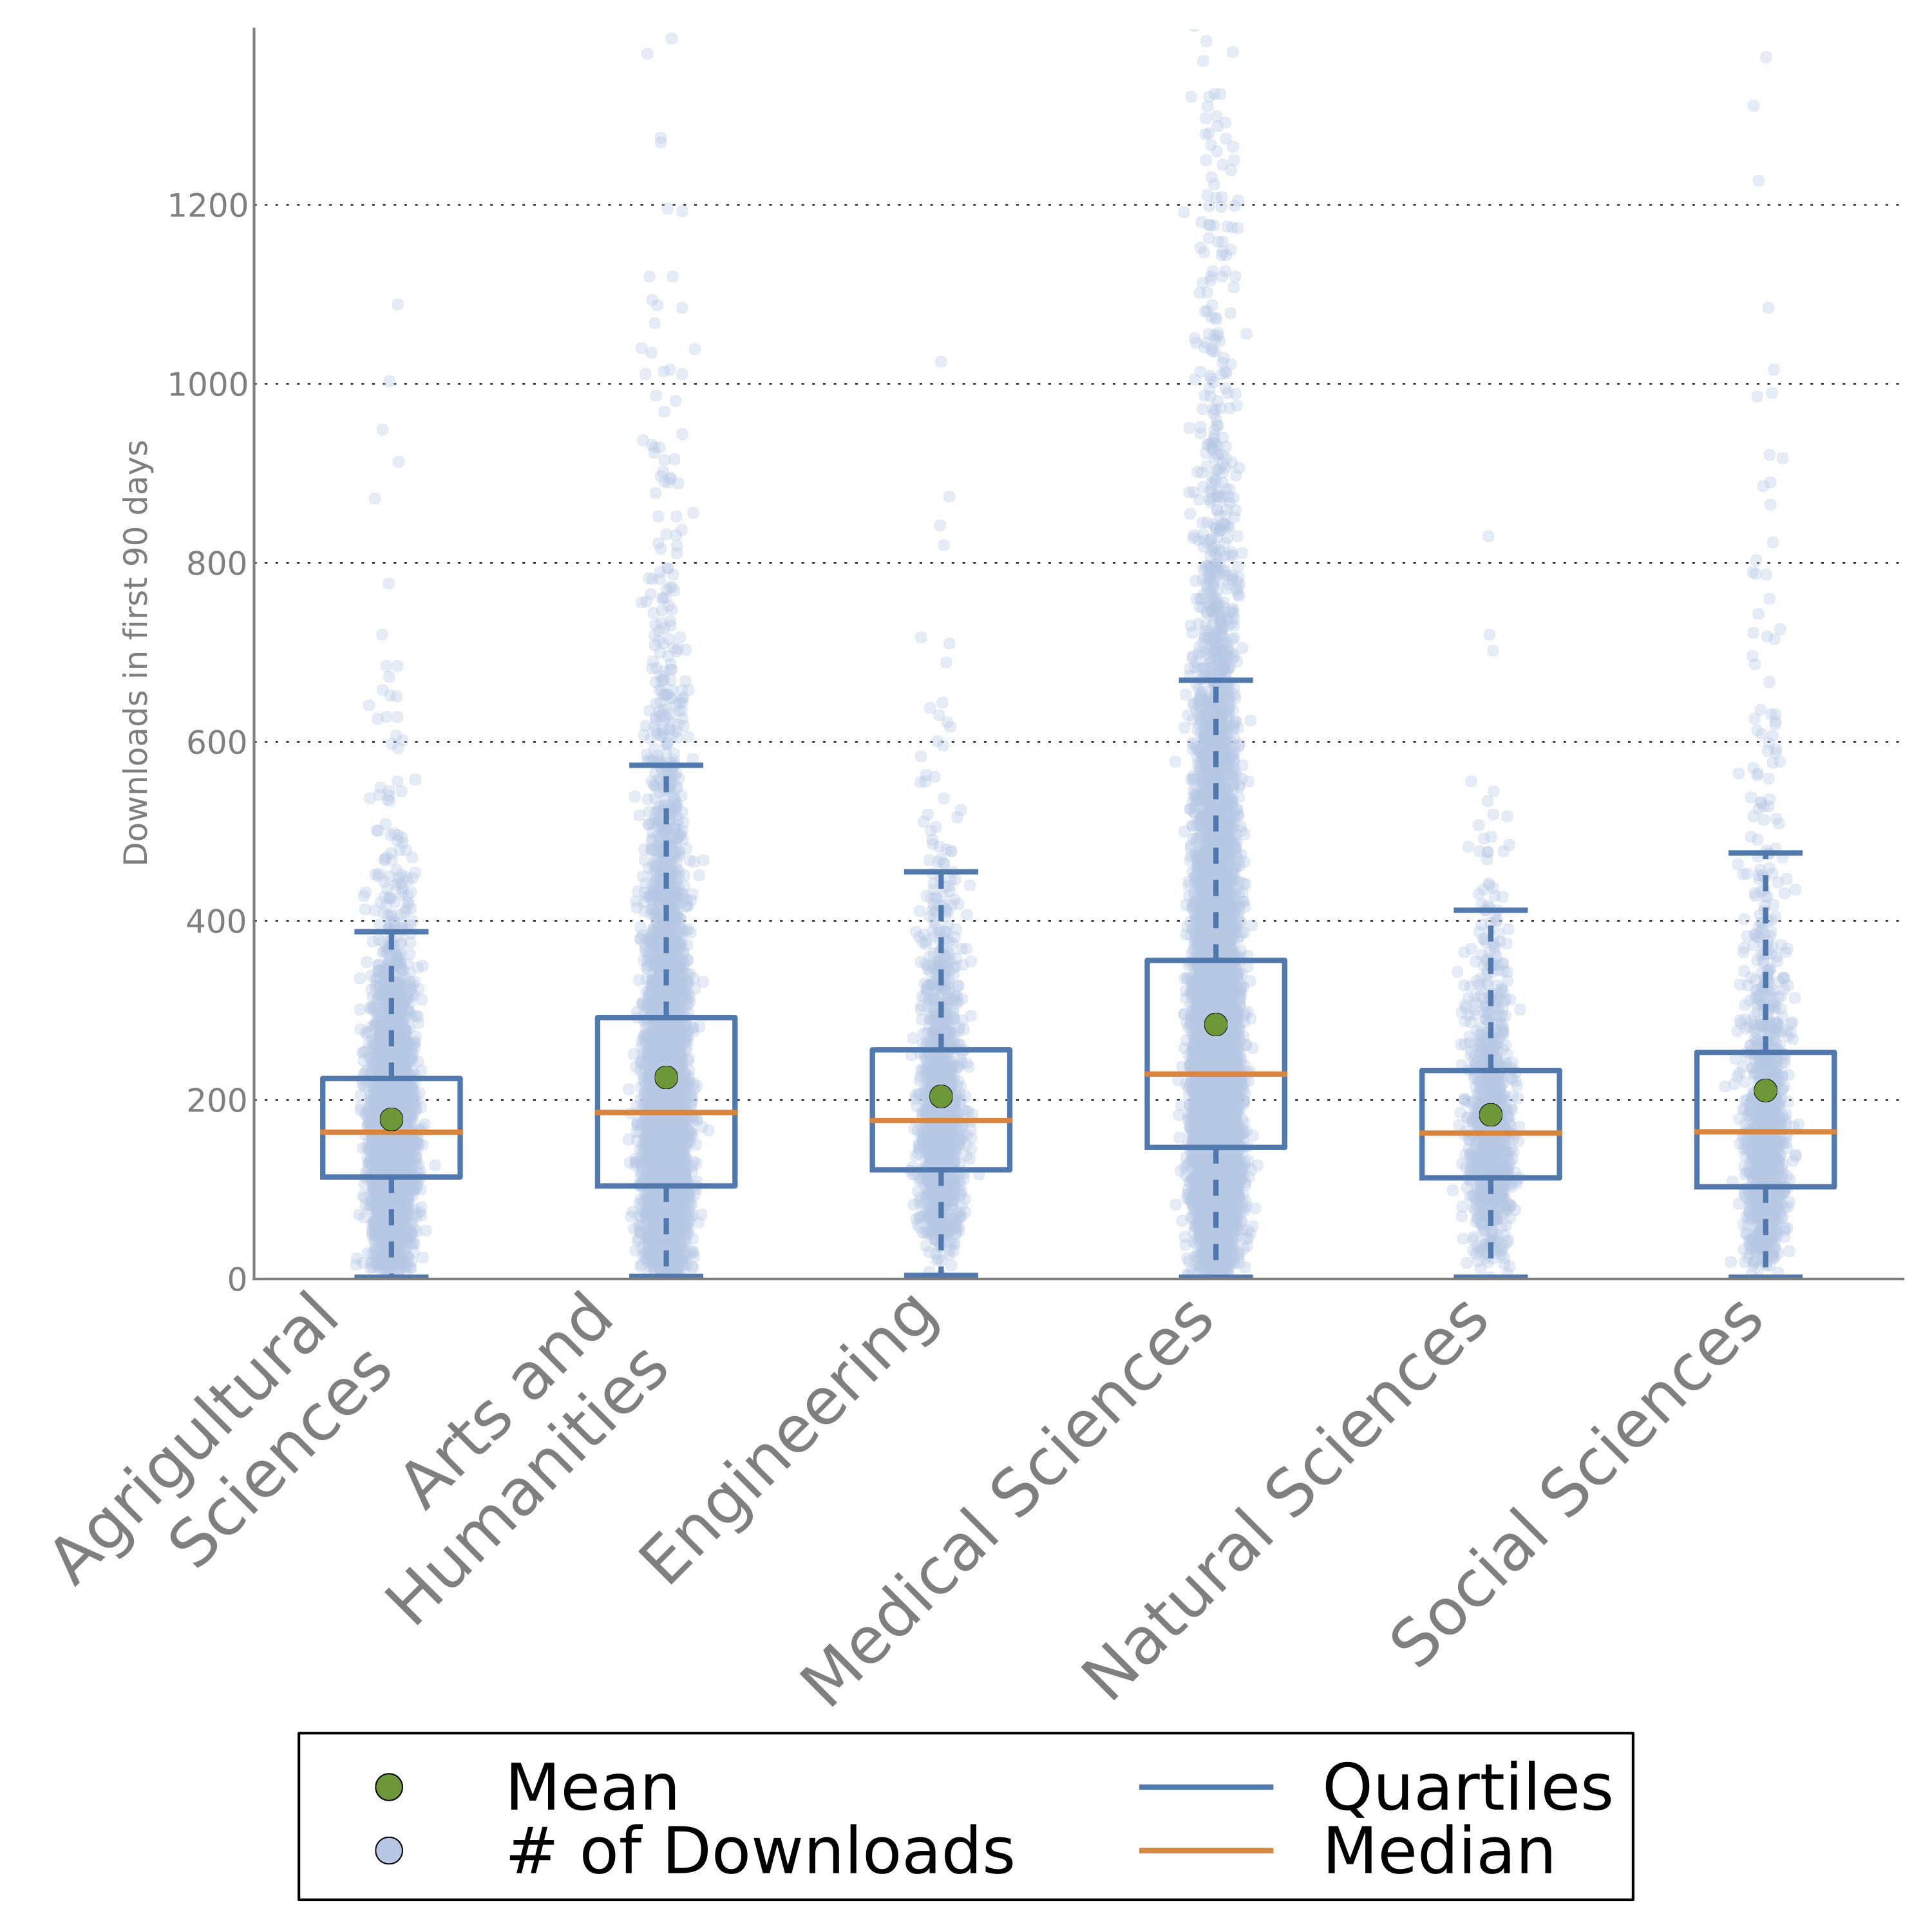
\includegraphics[keepaspectratio,width=\textwidth,height=0.45\textheight]{figures/downloads90_by_subject_scielo.png}
\caption{Distribution of Number of Downloads by Journal Discipline (SciELO)}
\label{downloads90_by_subject_scielo}
\end{figure}

\begin{figure}[htbp]
\centering
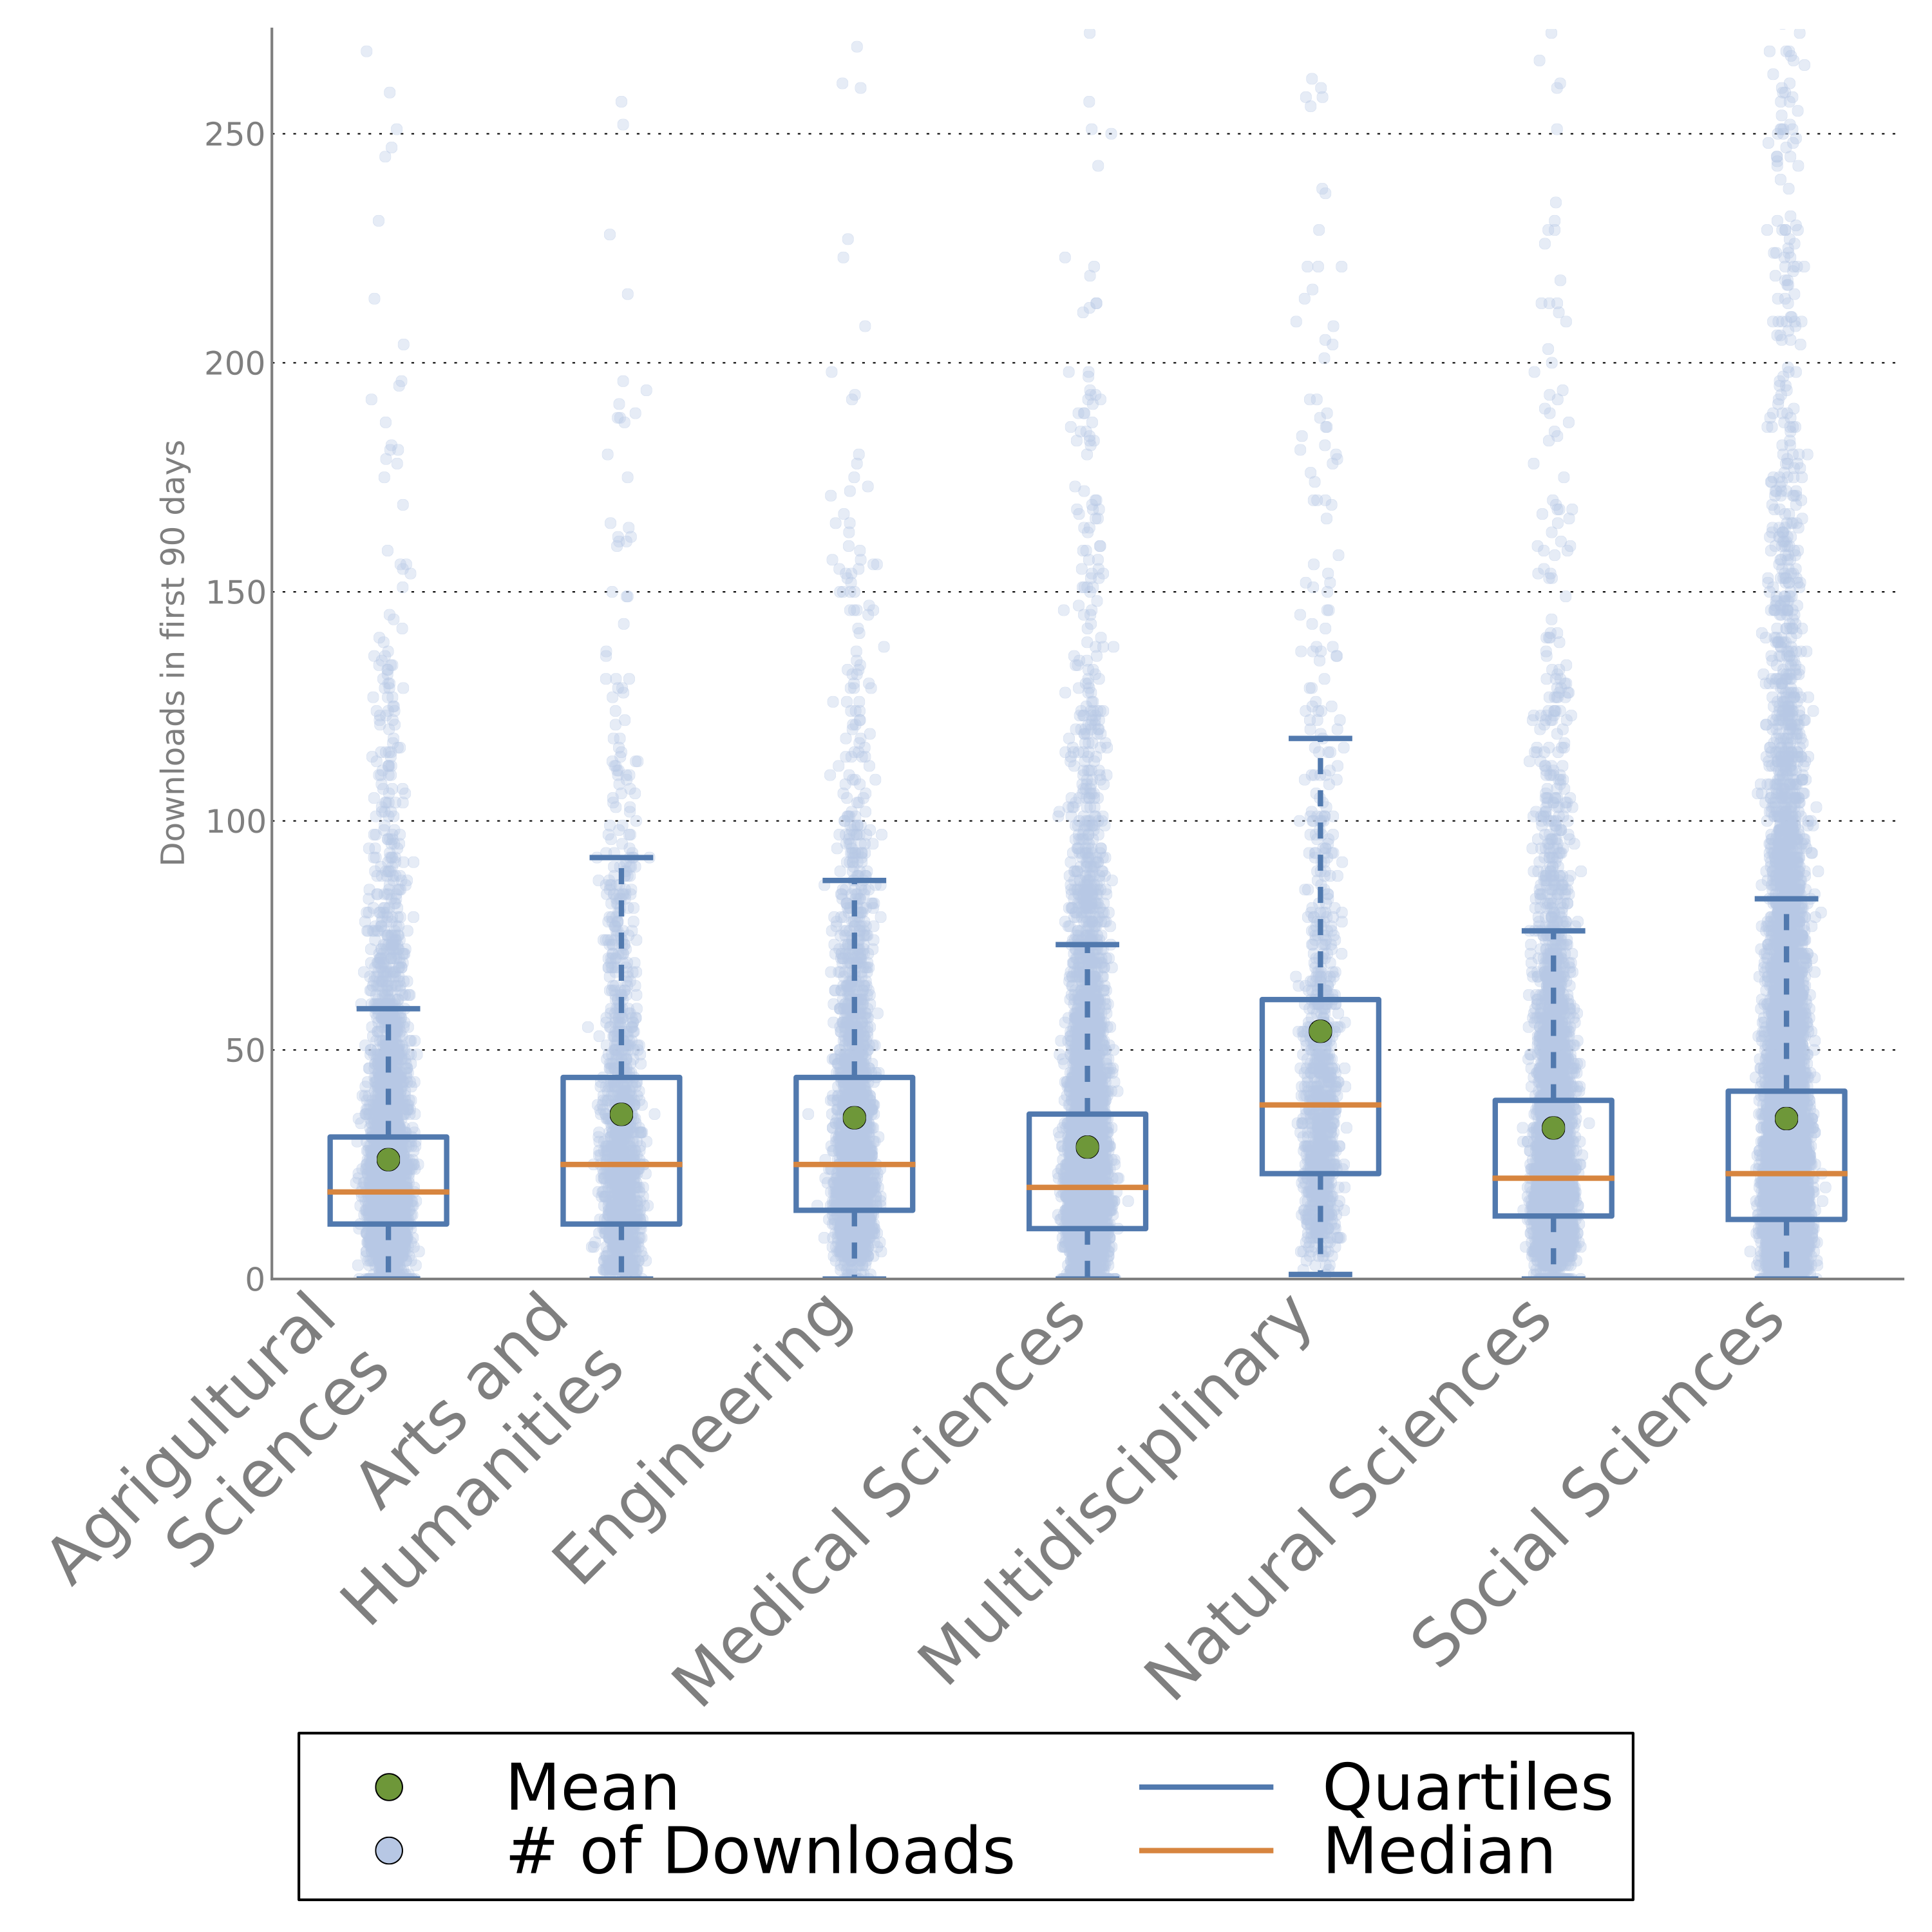
\includegraphics[keepaspectratio,width=\textwidth,height=0.45\textheight]{figures/downloads90_by_subject_redalyc.png}
\caption{Distribution of Number of Downloads by Journal Discipline (RedALyC)}
\label{downloads90_by_subject_redalyc}
\end{figure}

\begin{figure}[htbp]
\centering
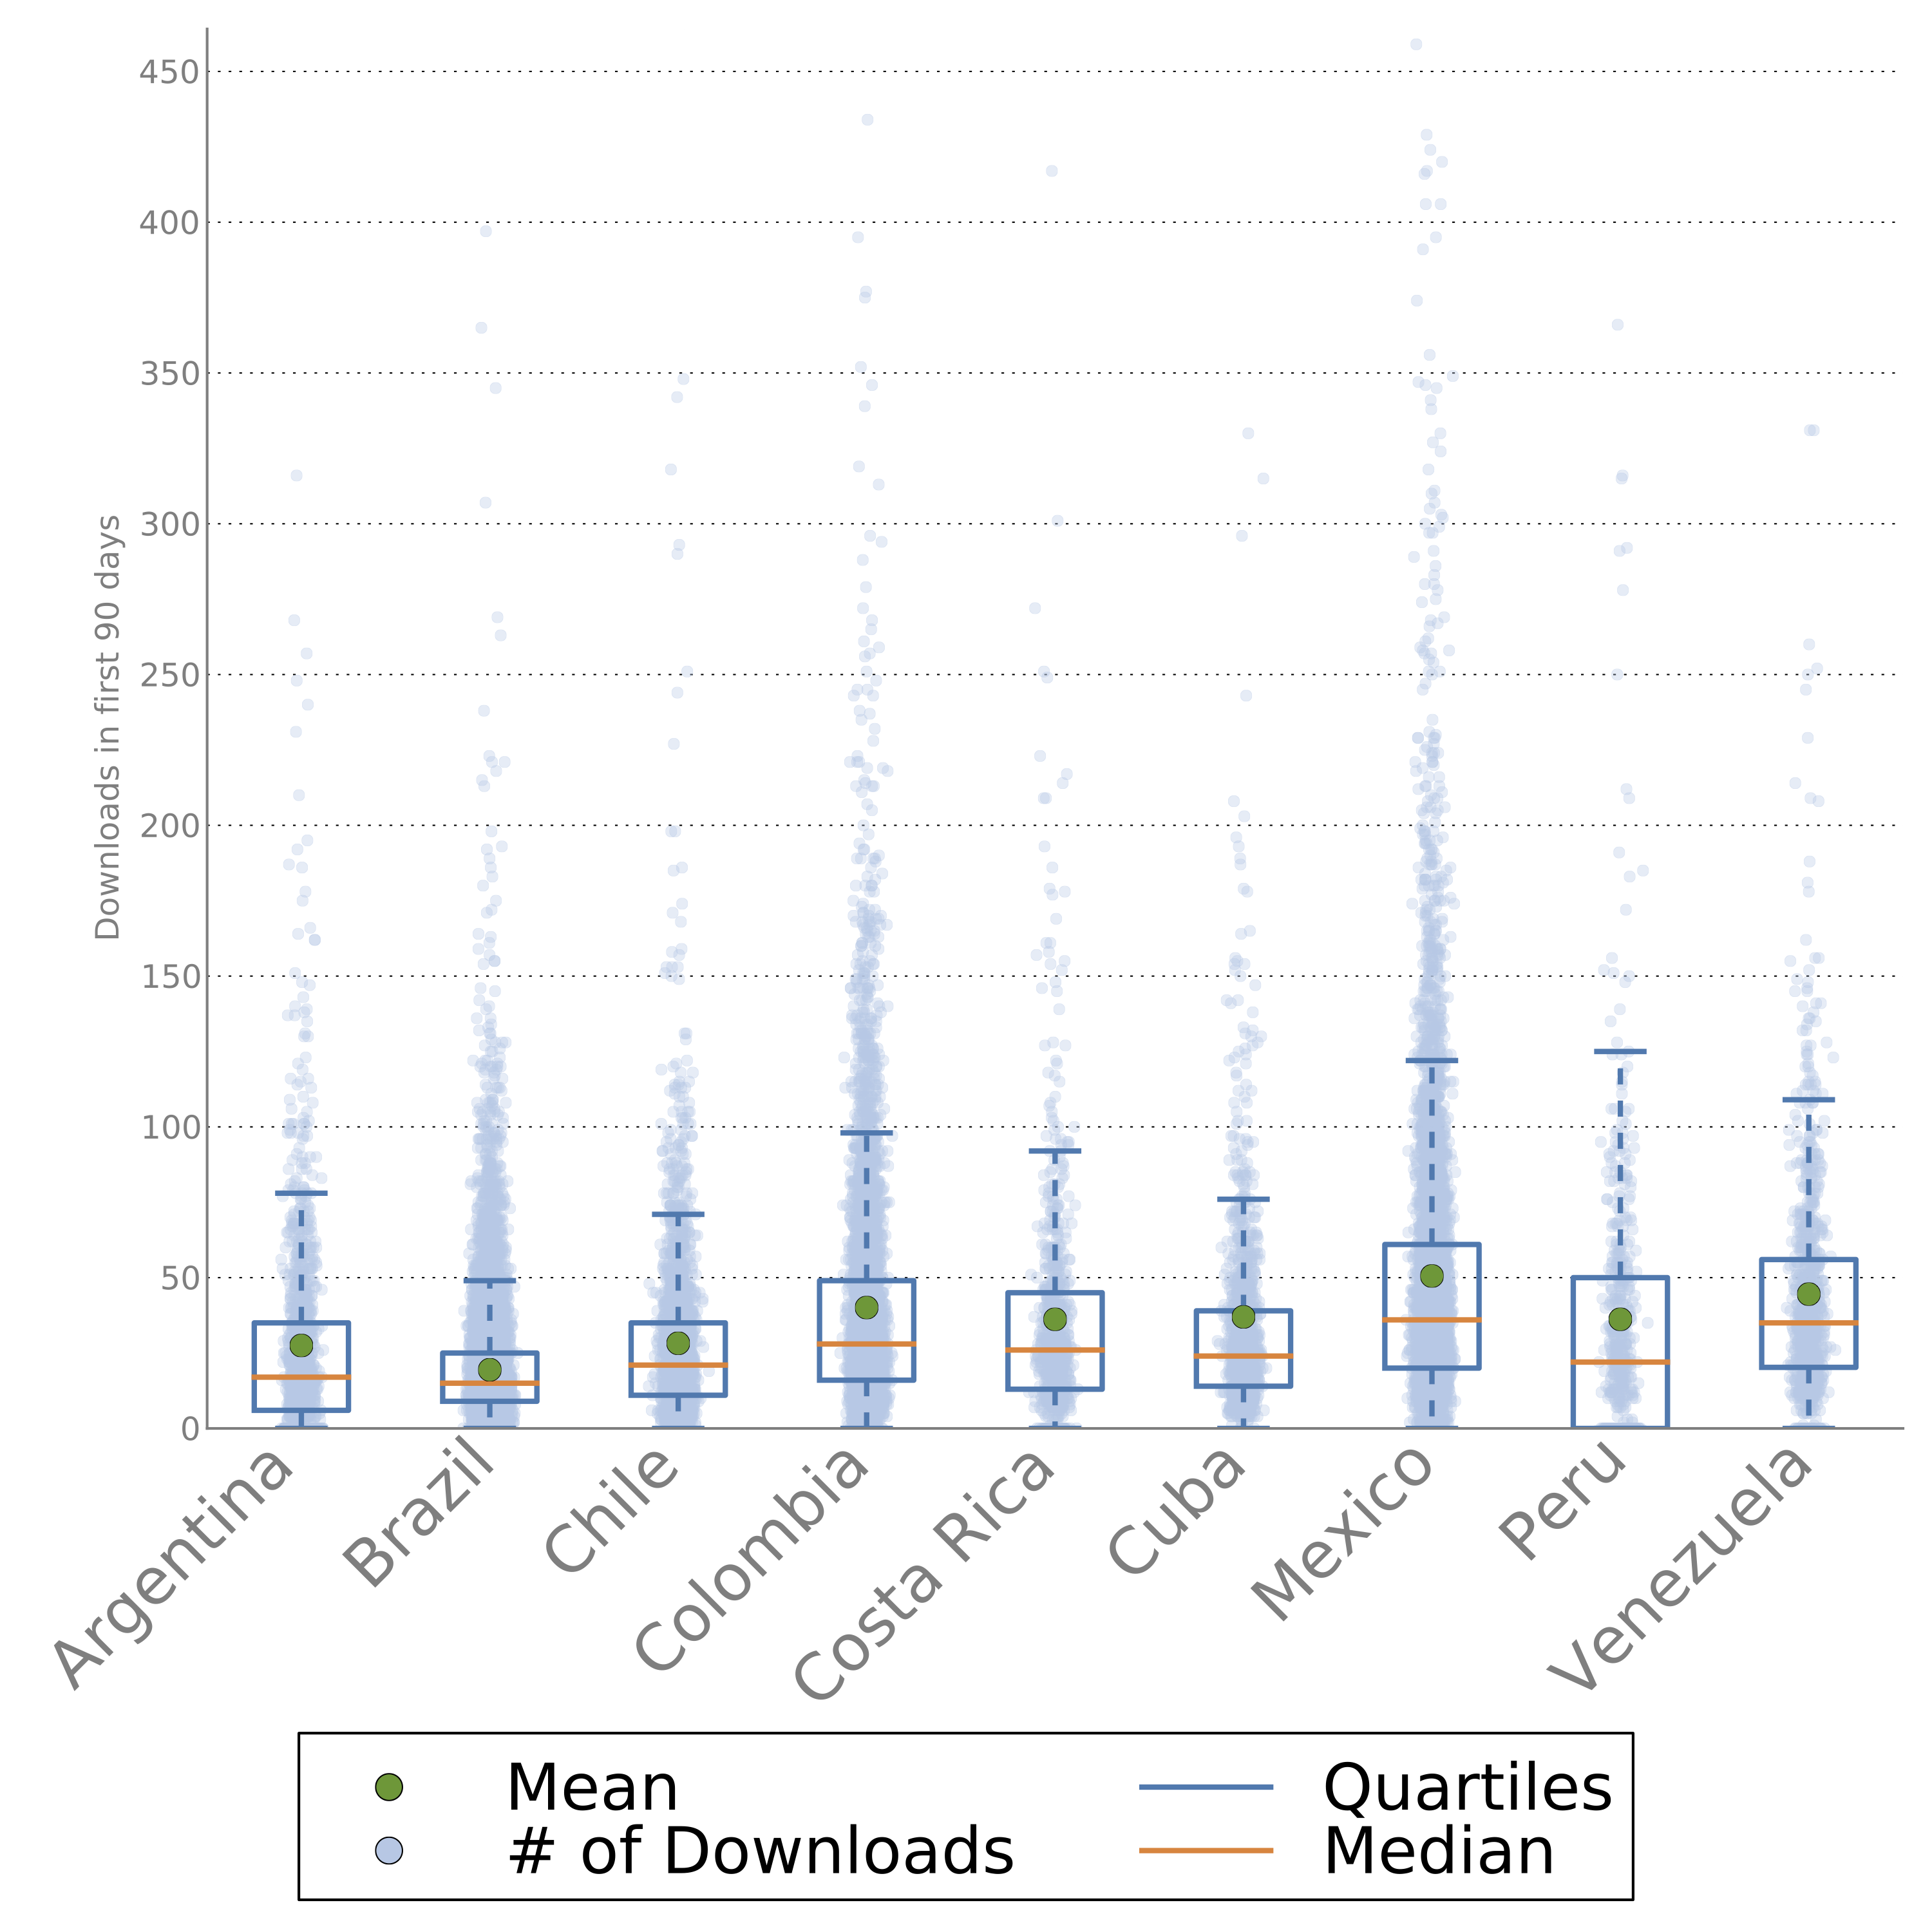
\includegraphics[keepaspectratio,width=\textwidth,height=0.45\textheight]{figures/downloads90_by_country_redalyc.png}
\caption{Distribution of Number of Downloads by Journal Country (RedALyC)}
\label{downloads90_by_country_redalyc}
\end{figure}

We can also link these responses to the survey responses from earlier to see if certain sectors are more likely to download highly downloaded articles. We can review the responses to Q1 and Q2 of the surveys, limiting the set of articles to those for which there is download data. This necessarily decreases the sample size of survey responses significantly, as it only considers the intersection of articles with download data and those associated with a survey response. In the case of RedALyC, this reduces the number of survey responses to around 1,700 (down from around 23,000) and in the case of SciELO to around 1,400 (down from around 55,000).

A comparison of mean and median number of downloads for each response, however, shows that the distribution of number of downloads is fairly similar across all responses (usage types). For RedALyC, the mean number of downloads ranges from 46 to 76 for Q1 and from 56 to 70 (Q2) and the medians range from 24 to 46 (Q1) and from 25 to 39 (Q2). Similarly, there is little variation between responses for the SciELO respondents. In that portal, the mean number of downloads ranges from 360 to 420 (Q1) and from 326 to 611 (Q2). The professional use does appear to have a higher mean than others, but the median value shows little variance between responses. A more detailed depiction of the spread can be seen in \autoref{downloads90_by_q1_q2_redalyc} for RedALyC and in \autoref{downloads90_by_q1_q2_scielo} for SciELO. It should be noted that in both cases the number of observations for some of the responses is small, decreasing the confidence of the calculated means.

\begin{figure}[htbp]
\centering
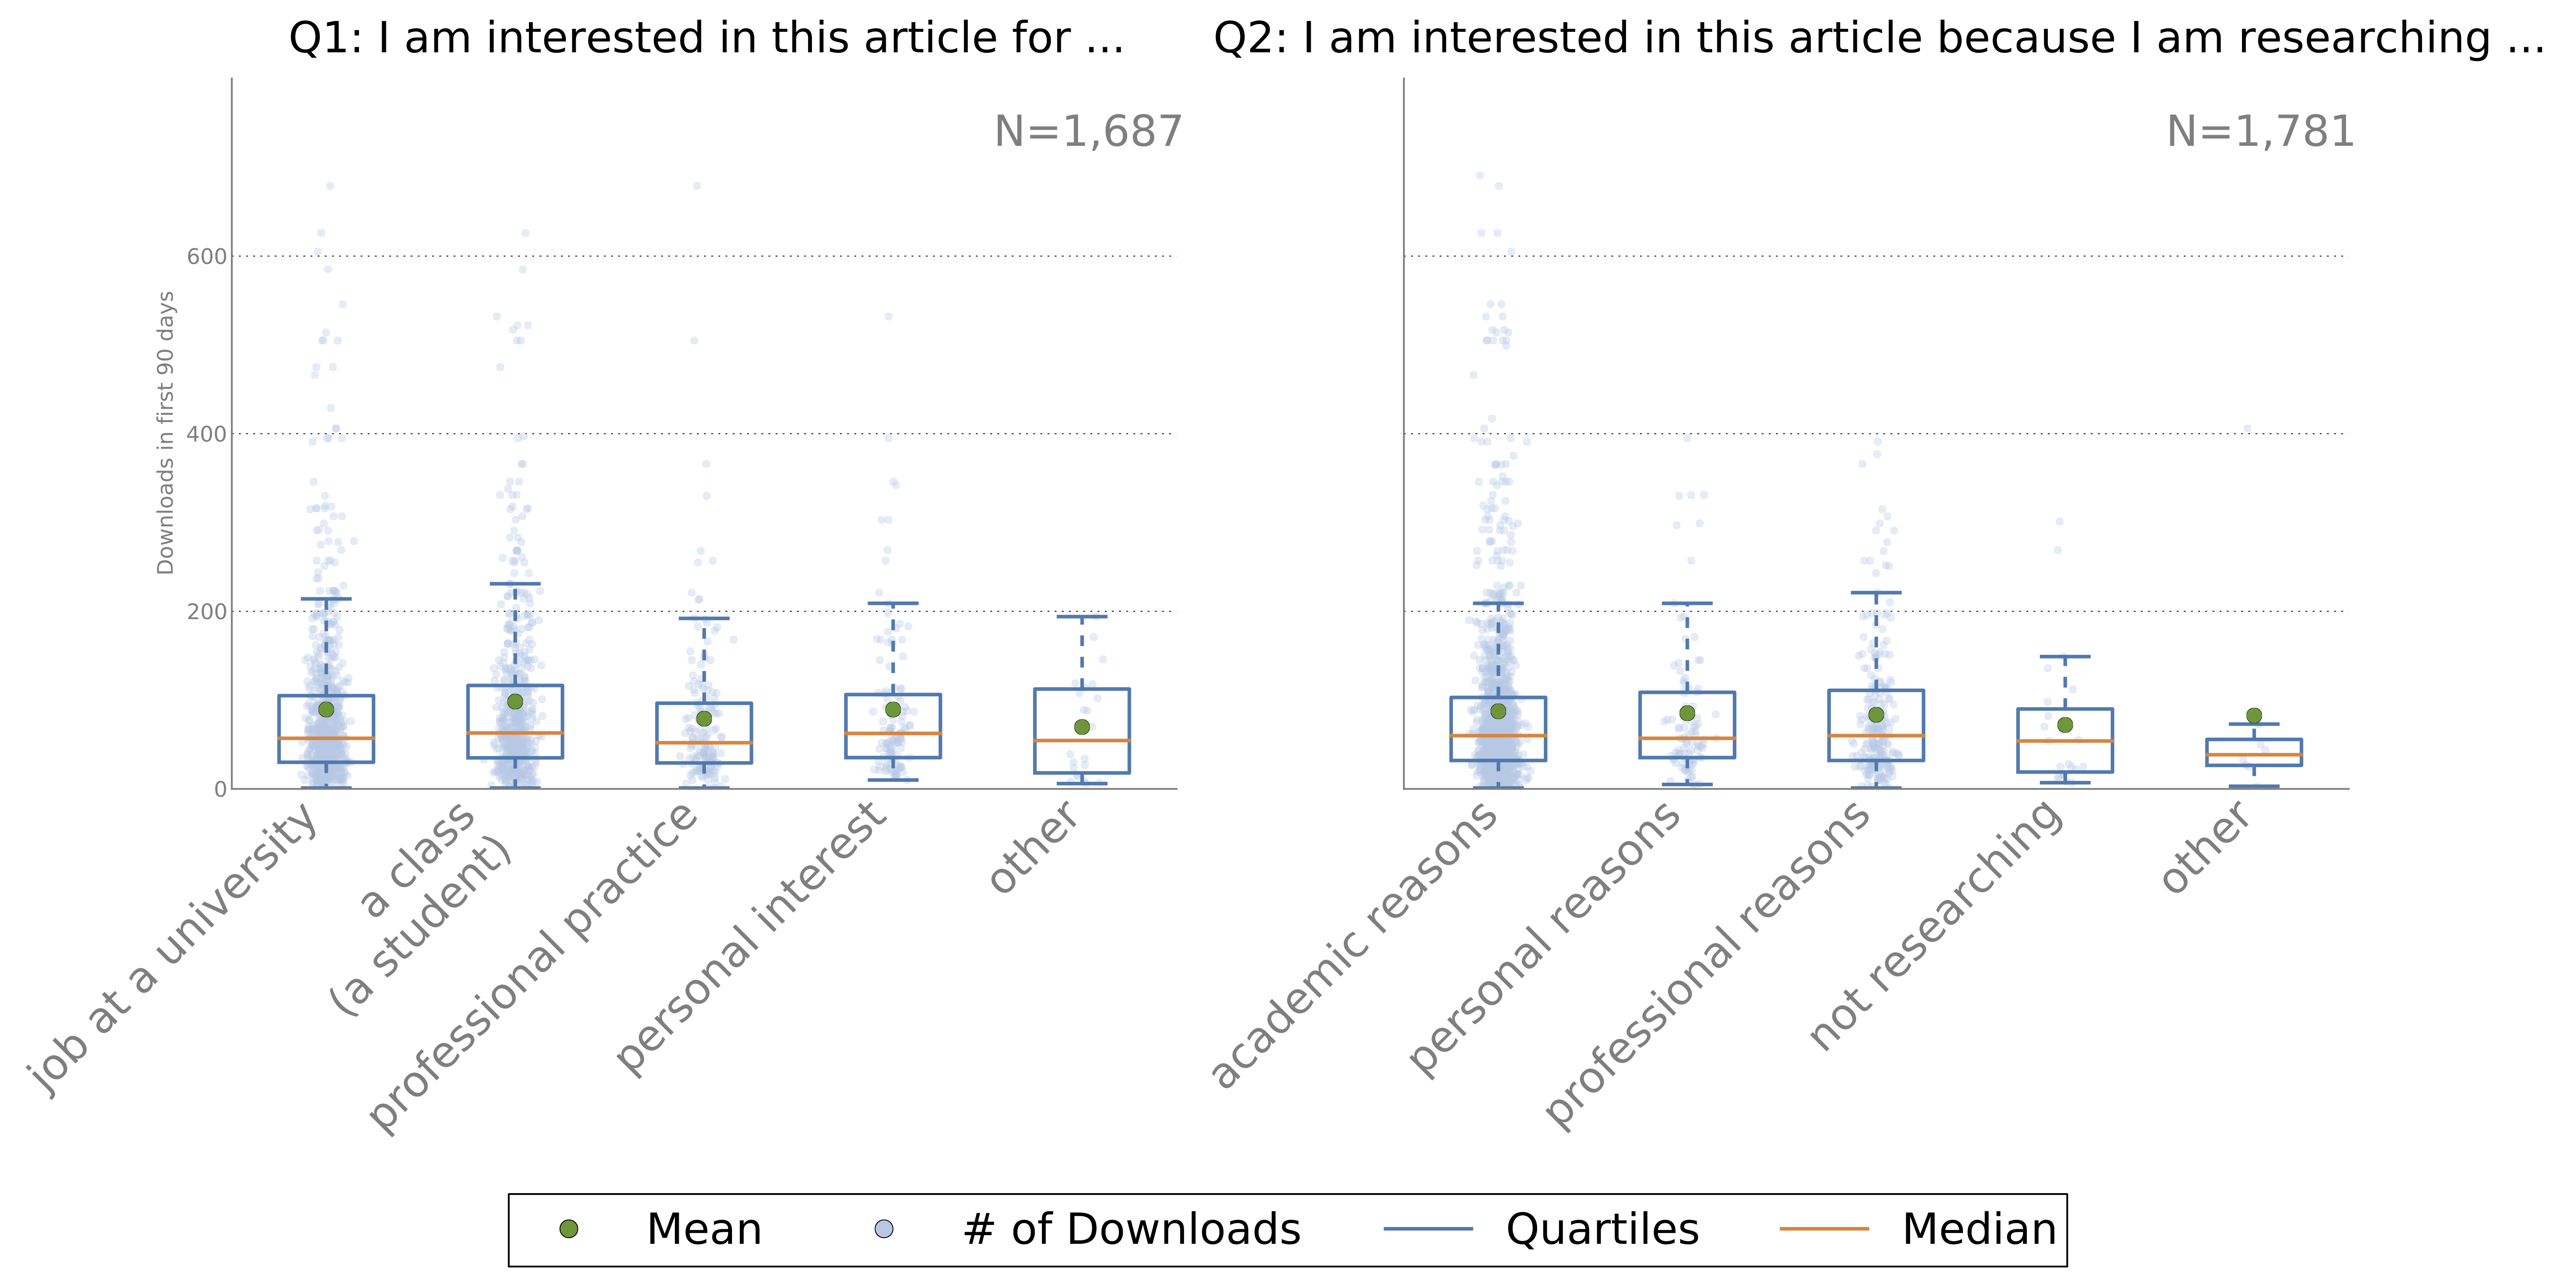
\includegraphics[keepaspectratio,width=\textwidth,height=0.75\textheight]{figures/downloads90_by_q1_q2_redalyc.png}
\caption{Distribution of Number of Downloads by Survey Response (RedALyC)}
\label{downloads90_by_q1_q2_redalyc}
\end{figure}

\begin{figure}[htbp]
\centering
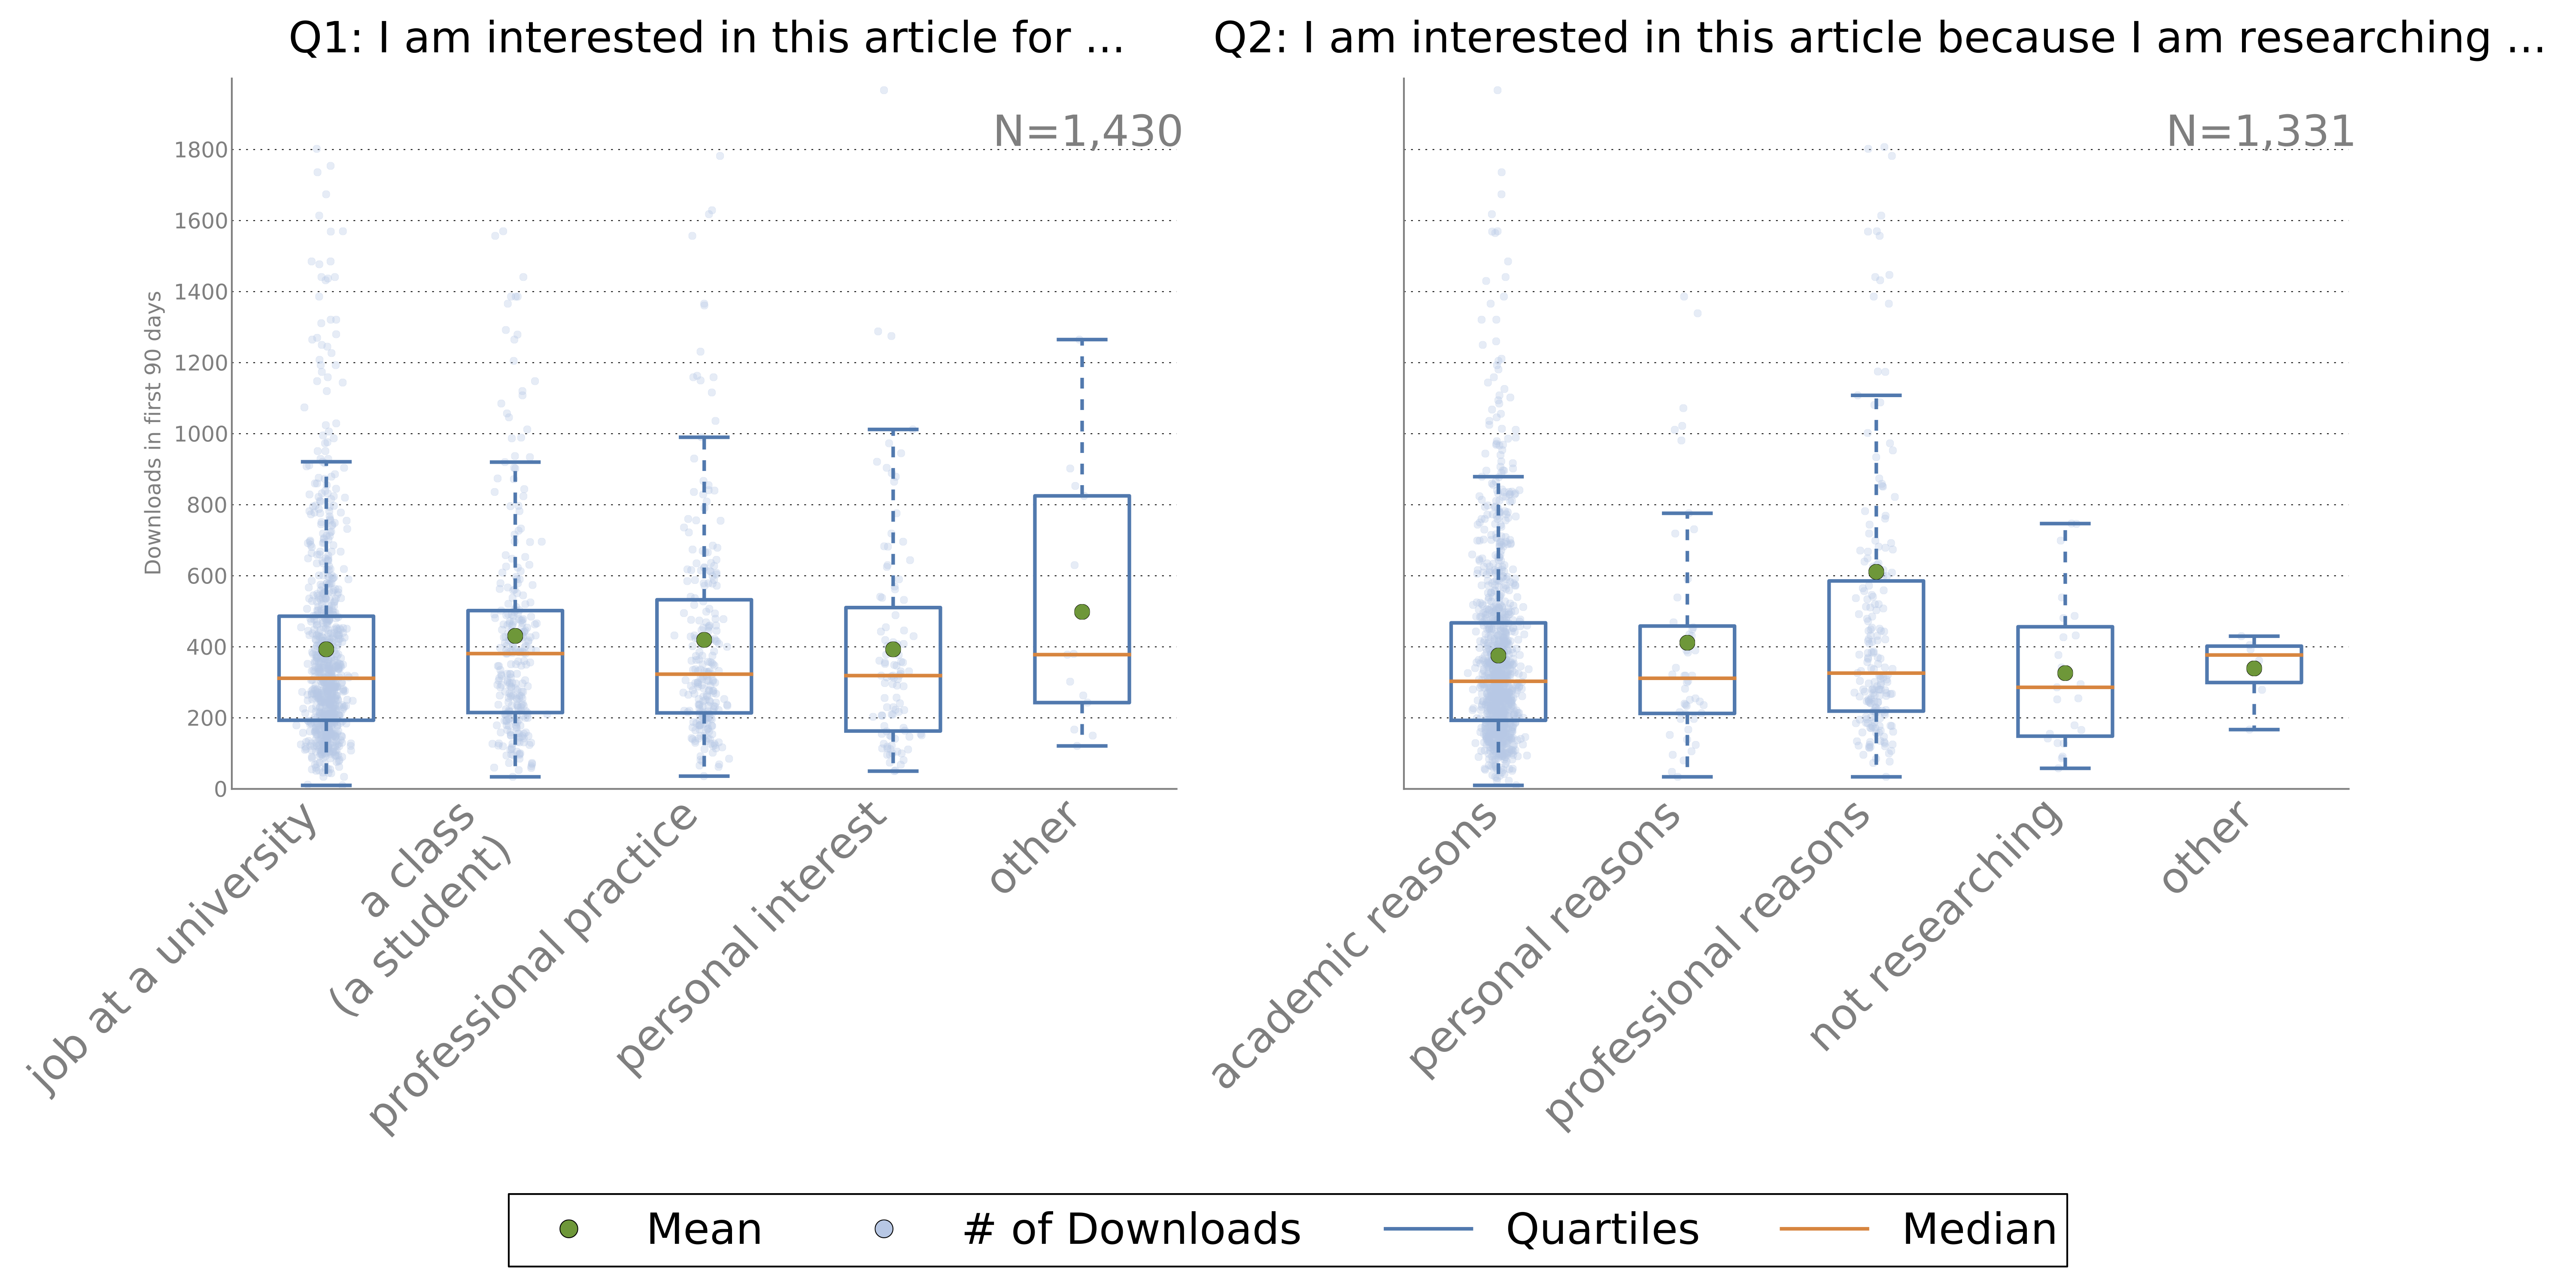
\includegraphics[keepaspectratio,width=\textwidth,height=0.75\textheight]{figures/downloads90_by_q1_q2_scielo.png}
\caption{Distribution of Number of Downloads by Survey Response (SciELO)}
\label{downloads90_by_q1_q2_scielo}
\end{figure}

\subsection{Summary}
\label{summary}

The pop-up polls and demographic surveys serve to paint, in fairly broad strokes, a picture of the users of Latin American research. The first thing that stands out is the high percentage of students, split fairly evenly between undergraduate and graduate, and indicative of a yet unmeasured pedagogical impact of Latin American research.

The second notable characteristic of the users of the research is the significant portion, somewhere between a sixth and a quarter, of non-academic use. This use, primarily stemming from professionally-related interests, comes from an almost exclusively university-educated public, working in both the public and private sector (and to a much lesser degree the non-profit sector). We do see some disciplinary differences, with the medical sciences the only clear example of a field that has particularly strong professional interest. It remains unknown whether the professionally-related interests is from individuals working in hospitals, research centres, private corporations, or government entities.

The same can be said for the other aspect of non-academic use, strictly personal interest. Although personal interest is not as prominent, it still makes up over 5\% of the total usage. In one of the portals, there is a topical focus on Arts and Humanities, although other fields also show similar levels of personal interest.

The topic models derived from looking at the titles of the articles being read by respondents of the first and second pop-up questions help characterize the content that is being researched by each group of respondents. We very clearly notice the importance of health-related topics, especially among readers researching to help with their jobs within the public sector and, in the case of the SciELO portal, also for readers coming for personal reasons.

Yet, despite the prevalence of health-related terms, each of the non-academic sectors appear to access articles with very different terms. Of the dimensions studied and described in the preceding sections (country of publication, language, and discipline, and topics), only discipline and topics show some consistency between both portals among the readers of each sector, and only the topic models show a completely consistent pattern between the users of both portals. Although the topics themselves vary between portals (something we expect given that the portals have different disciplinary distributions) the analysis of similarities in term distributions among each groups shows which groups are most similar to each other and which are most different.

In this analysis, we see that both the academic sectors are actually quite similar, and that private sector employees access topics that are most dissimilar from all others. All this suggests, as with the pop-up surveys themselves, that the audiences of Latin American research are quite varied. Not only do they come from different sectors and with different motivations, but they access different content and likely need a broader range of indicators of impact than citation-based measures.

The average usage of articles published is moderate in SciELO and low in RedALyC, with SciELO receiving around nine times the number of downloads, on average. Both portals also exhibit difference in which fields show higher and lower average download counts over the first 90 days since publication. SciELO shows a relative strength in the medical sciences, and RedALyC in multidisciplinary journals. However, these differences are not very pronounced, and the differences virtually disappear when looking at the median number of downloads.

In RedALyC, where the differences in downloads between country of publication can be observed, it appears that Mexican journals receive, on average, a higher number of downloads than articles published in journals from other countries. Again, this difference is not very pronounced.

Finally, when looking at the average number of downloads by survey response (type of user) there appears to be no significant difference in the average number of downloads for either portal.

\section{Impact}
\label{impact}

The understanding of the demographics of readers of Latin American research, their motivations, and a broad sense of their topics of interest are all indicative of varied types of readers with equally varied motivations for accessing Latin American research. While the download counts presented in the previous section give a sense of the extent of the reach of the reach, altmetrics offer the potential of capturing this impact, especially when considering that much of the use uncovered is by students and professionals—two groups who are not themselves authors and whose use of the literature would not be reflected in traditional citation-based measures of impact.

Altmetrics also present the opportunity for capturing the demographics of the users in a broad way, without the need for survey tools like those employed in this study. However, to be useful in either capacity, it is necessary for the metrics to be available across a broad range of articles. That is, there needs to be sufficient coverage of the published articles by altmetrics sources for the metrics to prove generally useful.

A comparison of coverage levels across both portals can only be done for the period since Altmetric began collecting data specific to both portals. This period spans between November 2013 and June 2014. We can measure coverage in two ways: 1) by looking at the raw number of social media mentions, and 2) by looking at the proportion of articles that receive mentions.

The first thing to note is that for both the SciELO and RedALyC portals, the Altmetric.com source with the most mentions, by a significant margin, is Twitter. Facebook also has a significant number of articles with mentions, and Google+ and Videos have a few. All other sources are virtually zeros everywhere (\autoref{altmetric_raw_counts_Nov2013_May2014_scielo} and \autoref{altmetric_raw_counts_Nov2013_May2014_redalyc}).\footnote{Other sources not listed here, such as Pinterest and LinkedIn had no mention in either portal.}

As can be seen in the tables above, the Brazilian journals on SciELO have far larger number of mentions than any other country's journals on either portal. However, SciELO Brazil is also the largest, by more than four times the next largest country collection and therefore has a less than 1\% coverage rate. When looking at coverage in this way, as a proportion, Cuban journals in RedALyC has the highest coverage with 3.42\% of articles having at least one mention in any source. In fact, the Cuban journals in RedALyC are the only collection that has over 2\% coverage.\footnote{Its worth repeating that these numbers are based only on mentions that occurred between November 1st, 2013 and May 31st, 2014, a period that spans the Christmas and the summer holidays in the Southern hemisphere, as well as Carnaval in Brazil.}

The immediacy of mentions is also an important factor, and one that will come into play in the subsequent analysis. SciELO articles have the expected pattern of higher mentions for more recent publications, whereas RedALyC articles tend to be mentioned at about the same rate for any date of publication past 2007 (\autoref{altmetrics_coverage_by_year_both}).\footnote{The dip in 2014 in the RedALyC data may be explained by the bulk-uploading pattern of RedALyC, which may have occurred late in the period studied. In contrast, SciELO uploads articles on a continuous basis.} Because of the low levels of coverage in this dataset, below 1\% for all years prior to 2013, we turn our attention to the SciELO Brazil articles, for which an extended dataset which spans mentions that occurred during all of 2013 is available. This extended dataset has also been complemented with data for mentions in Wikipedia and of saves in the Mendeley reference manager.



\begin{sidewaystable}[!htbp]
\centering
\begin{threeparttable}
\caption{Altmetric.com Mentions of SciELO Articles} \label{altmetric_raw_counts_Nov2013_May2014_scielo}
\begin{tabular}{@{}lcccccccc@{}}
\toprule
Country &   N   &   Blogs   &   Facebook    &   Google+ &   Mass Media  &   Twitter &   Videos  &   Any Altmetric   \\ \midrule
Argentina   &   21,507   &   0   &   32  &   0   &   0   &   216 &   3   &   244 \\
Brasil  &   22,4292  &   6   &   551 &   32  &   6   &   1,402    &   36  &   1,935    \\
Chile   &   38,988   &   0   &   31  &   5   &   0   &   568 &   3   &   595 \\
Colombia    &   35,736   &   0   &   4   &   2   &   0   &   136 &   1   &   141 \\
Costa Rica  &   4,592    &   1   &   0   &   0   &   1   &   44  &   0   &   46  \\
Cuba    &   19,535   &   0   &   7   &   4   &   0   &   208 &   2   &   218 \\
México &   24,205   &   0   &   18  &   2   &   0   &   207 &   0   &   223 \\
Perú   &   5,388    &   0   &   3   &   1   &   0   &   51  &   0   &   53  \\
Venezuela   &   15,552   &   0   &   4   &   2   &   0   &   187 &   0   &   192 \\ \midrule
Total   &   389,795  &   7   &   650 &   48  &   7   &   3,019    &   45  &   3,647    \\ \bottomrule
\end{tabular}
\begin{tablenotes}
\small
\item Note: Table shows a raw count of number of mentions of articles in any of the scielo domains that occurred between November 2013 and May 2014.
\end{tablenotes}
\end{threeparttable}
\end{sidewaystable}

\begin{sidewaystable}[!htbp]
\centering
\begin{threeparttable}
\caption{Altmetric.com Mentions of Redalyc.org Domain} \label{altmetric_raw_counts_Nov2013_May2014_redalyc}
\begin{tabular}{@{}lcccccccc@{}}
\toprule
Country &   N   &   Blogs   &   Facebook    &   Google+ &   Mass Media  &   Twitter &   Videos  &   Any Altmetric   \\ \midrule
Argentina   &   7,896    &   0   &   3   &   0   &   0   &   25  &   0   &   26  \\
Bolivia &   26  &   0   &   0   &   0   &   0   &   0   &   0   &   0   \\
Brasil  &   66,461   &   0   &   5   &   2   &   0   &   31  &   0   &   38  \\
Chile   &   15,942   &   0   &   1   &   4   &   0   &   50  &   0   &   55  \\
Colombia    &   36,228   &   0   &   4   &   6   &   0   &   139 &   1   &   147 \\
Costa Rica  &   5,202    &   0   &   1   &   1   &   0   &   20  &   0   &   22  \\
Cuba    &   9,071    &   0   &   1   &   0   &   0   &   309 &   0   &   310 \\
Ecuador &   230 &   0   &   0   &   0   &   0   &   4   &   0   &   4   \\
México &   43,858   &   1   &   9   &   10  &   0   &   158 &   1   &   175 \\
Perú   &   3,481    &   0   &   0   &   1   &   0   &   15  &   0   &   16  \\
Puerto Rico &   265 &   0   &   0   &   0   &   0   &   2   &   0   &   2   \\
República Dominicana   &   285 &   0   &   0   &   0   &   0   &   0   &   0   &   0   \\
Uruguay &   81  &   0   &   0   &   0   &   0   &   0   &   0   &   0   \\
Venezuela   &   11,993   &   0   &   3   &   4   &   0   &   92  &   0   &   99  \\ \midrule
Total   &   201,019  &   1   &   27  &   28  &   0   &   845 &   2   &   894 \\ \bottomrule
\end{tabular}
\begin{tablenotes}
\small
\item Note: Table shows a raw count of number of mentions of articles in the redalyc.org domain that occurred between November 2013 and May 2014.
\end{tablenotes}
\end{threeparttable}
\end{sidewaystable}

\begin{table}[!htbp]
\centering
\caption{Altmetric.com Coverage by Article Publication Year} \label{altmetrics_coverage_by_year_both}
\begin{tabular}{@{}lcccc@{}}
\toprule
    &\multicolumn{2}{c}{SciELO} &\multicolumn{2}{c}{RedALyC}  \\ \cmidrule(l{2pt}r{2pt}){2-3} \cmidrule(l{2pt}r{2pt}){4-5}
    &   Number of&  Proportion of   & Number of &   Proportion of \\
Year    &   Mentions    & Articles  & Mentions &    Articles \\ \midrule
2000    &   76  &   0.81\%  &   12  &   0.36\%  \\
2001    &   78  &   0.68\%  &   8   &   0.19\%  \\
2002    &   95  &   0.68\%  &   11  &   0.20\%  \\
2003    &   97  &   0.60\%  &   21  &   0.31\%  \\
2004    &   114 &   0.60\%  &   25  &   0.27\%  \\
2005    &   143 &   0.64\%  &   38  &   0.26\%  \\
2006    &   197 &   0.75\%  &   62  &   0.37\%  \\
2007    &   199 &   0.67\%  &   108 &   0.60\%  \\
2008    &   224 &   0.67\%  &   91  &   0.46\%  \\
2009    &   239 &   0.65\%  &   84  &   0.47\%  \\
2010    &   299 &   0.76\%  &   91  &   0.50\%  \\
2011    &   331 &   0.80\%  &   89  &   0.47\%  \\
2012    &   381 &   0.91\%  &   124 &   0.54\%  \\
2013    &   849 &   2.10\%  &   126 &   0.58\%  \\ \midrule
2014    &   325 &   3.83\%  &   4   &   0.11\%  \\ \midrule
Total   &   3,647   &   0.94\%  &   894 &   0.44\%  \\ \bottomrule
\end{tabular}
\end{table}




\subsection{SciELO Brazil}
\label{scielobrazil}

The number of SciELO Brazil articles from 2013 with some altmetrics is still quite low. Several of the categories did not have any mentions (LinkedIn, Reddit, Pinterest, Q\&A, Peer Review). Other categories also had less than 0.01\% coverage ($<$ 20 articles) (news, blogs, Google+, F1000, and Video, and Wikipedia). The only three sources with any significant number of mentions were Mendeley, Twitter, and Facebook.\footnote{As described in the previous chapter, the Altmetric.com data was complemented with data from Mendeley and Wikipedia for SciELO Brazil.} Across sources 5319 (25.09\%) of articles had at least one metric, but if Mendeley is excluded, only 1701 (8.02\%) have at least one metric.

\autoref{altmetrics_coverage_scielo_br} summarizes the levels of coverage for these three main metrics over all articles. There were 3,986 (18.80\%) articles with at least one Mendeley reader, 1,286 (6.03\%) with at least one Tweet, and 596 (2.81\%) articles with a Facebook public wall post.

The levels of coverage do vary by journal, with a handful of journals exhibiting nearly universal coverage. On average, 15.3\% of a journal's articles had at least one Mendeley reader (st. dev. 20.0), 5.8\% of journal's articles had at least one tweet (st. dev. 9.3), and 3.14\% of a journal's articles had at least one Facebook post (st. dev. 4.5). The spread of coverage can be seen in \autoref{altmetrics_coverage_scielo_br}. In all three cases, there are numerous journals that extend well beyond the 75\% percentile, potentially indicative of a marked difference in user communities or potentially a different promotion and diffusion strategies employed by the journals.



\begin{sidewaystable}[!htbp]
\centering
\caption{Summary of Mendeley, Twitter and Facebook for SciELO Brazil} \label{altmetrics_summary_main_metrics_scielo_br}
\begin{tabular}{@{}lccccccc@{}}
\toprule
Metric  &   Number of   &   Coverage (\%)   &   Maximum &   Mean    &   Standard    &   Mean    &   Standard    \\
        &   Articles    &               &           &           &   Deviation   &           &   Deviation   \\
        &               &               &           &           &               &   (metric > 0) &  (metric > 0)            \\ \midrule
Mendeley    &   3,986   &   18.8    &   119 &   0.59    &   2.06    &   3.15    &   3.8 \\
Twitter &   1,286   &   6.07    &   50  &   0.12    &   0.83    &   2.05    &   2.72    \\
Facebook    &   602 &   2.84    &   48  &   0.04    &   0.45    &   1.52    &   2.2 \\ \bottomrule
\end{tabular}
\end{sidewaystable}


The relationship between coverage and number of mentions in all three sources can be viewed by plotting the coverage levels against the mean number of mentions, which reveals a fairly strong correlation between the level of coverage a journal receives (y-axes) and the mean number of saves\slash mentions received by the articles in that journal (x-axes). This correlation is confirmed through an ordinary least-squares regression that results in R-squares of 0.69 for Mendeley, 0.77 for Twitter, and 0.82 for Facebook (\autoref{altmetrics_coverage_v_mean_scielo_br}). This is perhaps unsurprising given that the mean number of mentions is so low in most cases, so each mention is likely the first for the article, simultaneously increasing the journal's coverage and mean number by one.


\begin{figure}[htbp]
\centering
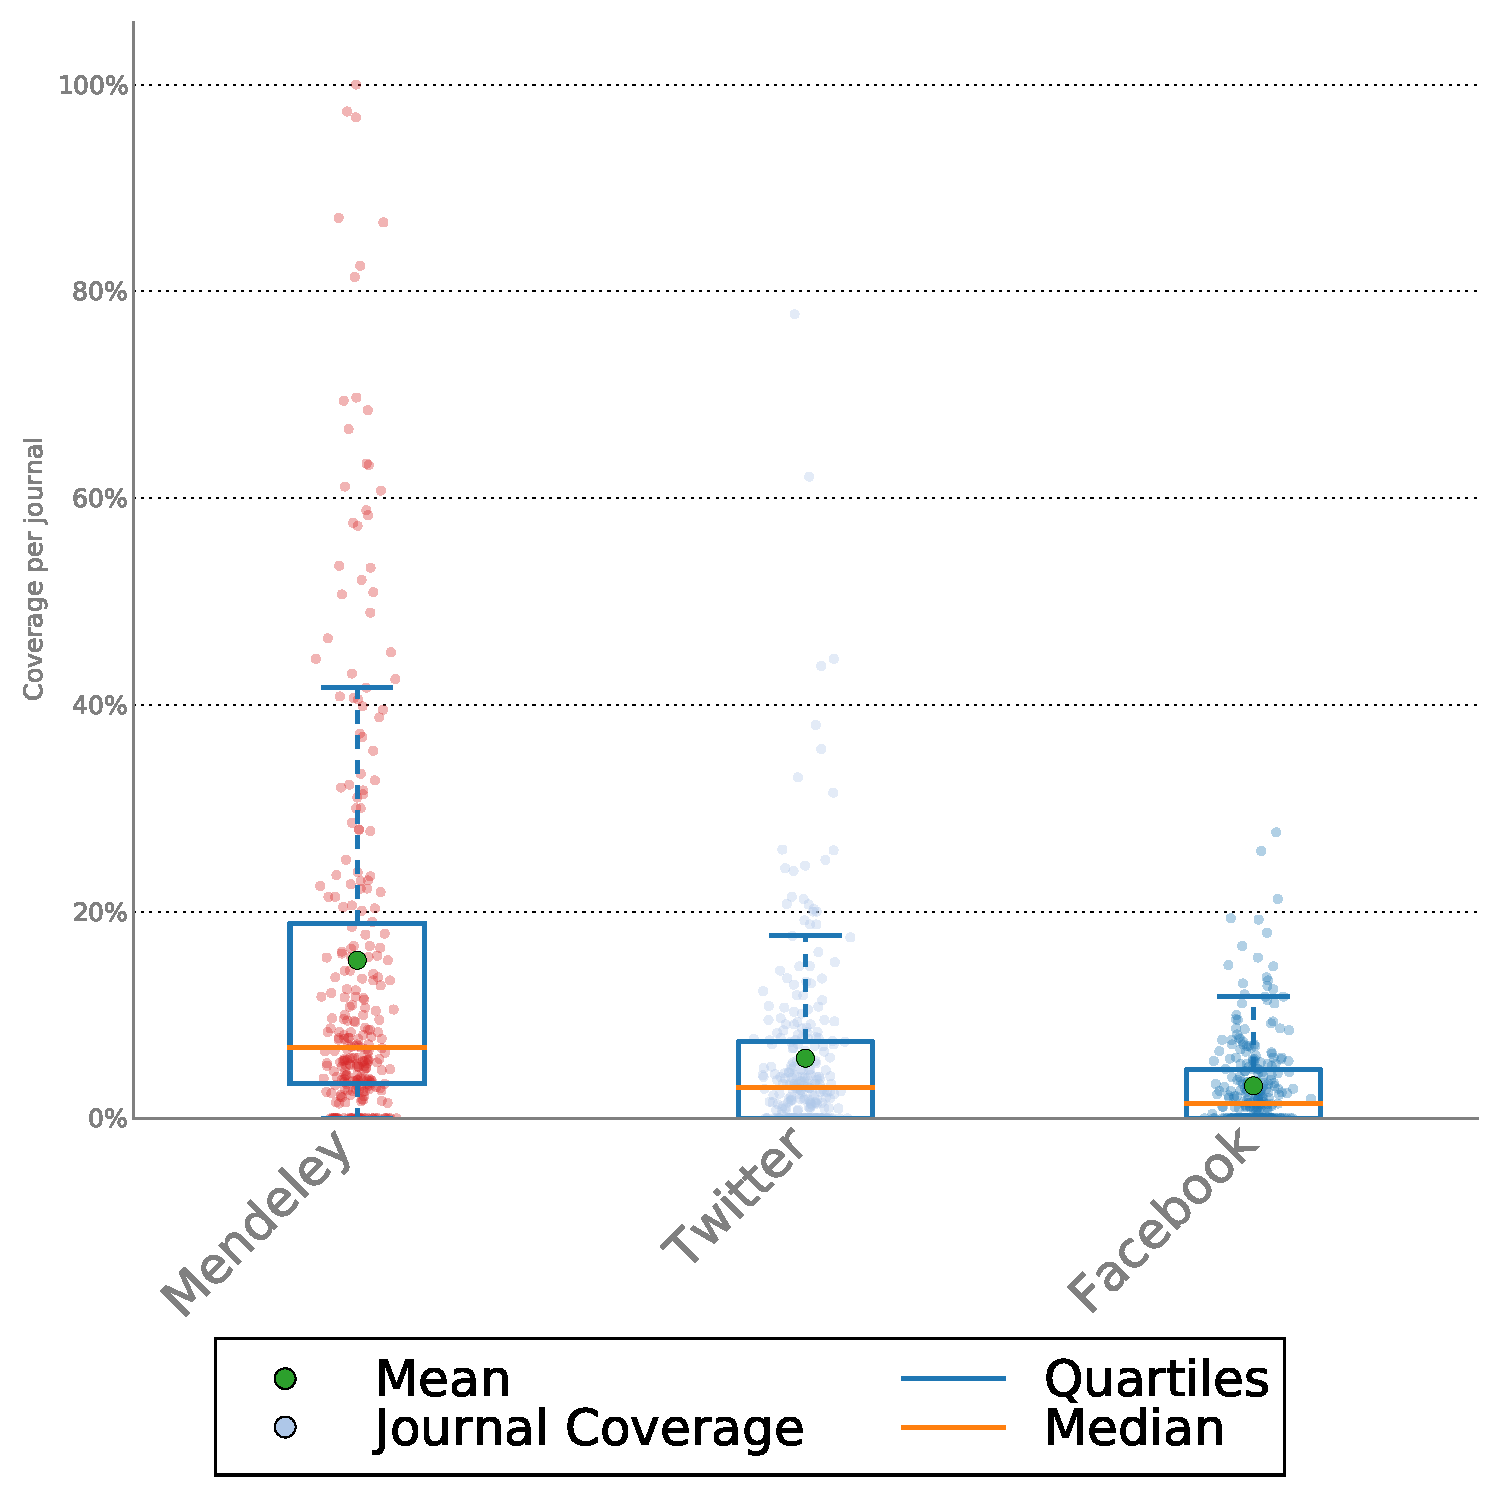
\includegraphics[keepaspectratio,width=\textwidth,height=0.45\textheight]{figures/altmetrics_coverage_scielo_br.pdf}
\caption{Percentage of 2013 Articles with at Least One Metric by Journal from SciELO Brazil}
\label{altmetrics_coverage_scielo_br}
\end{figure}

\begin{figure}[htbp]
\centering
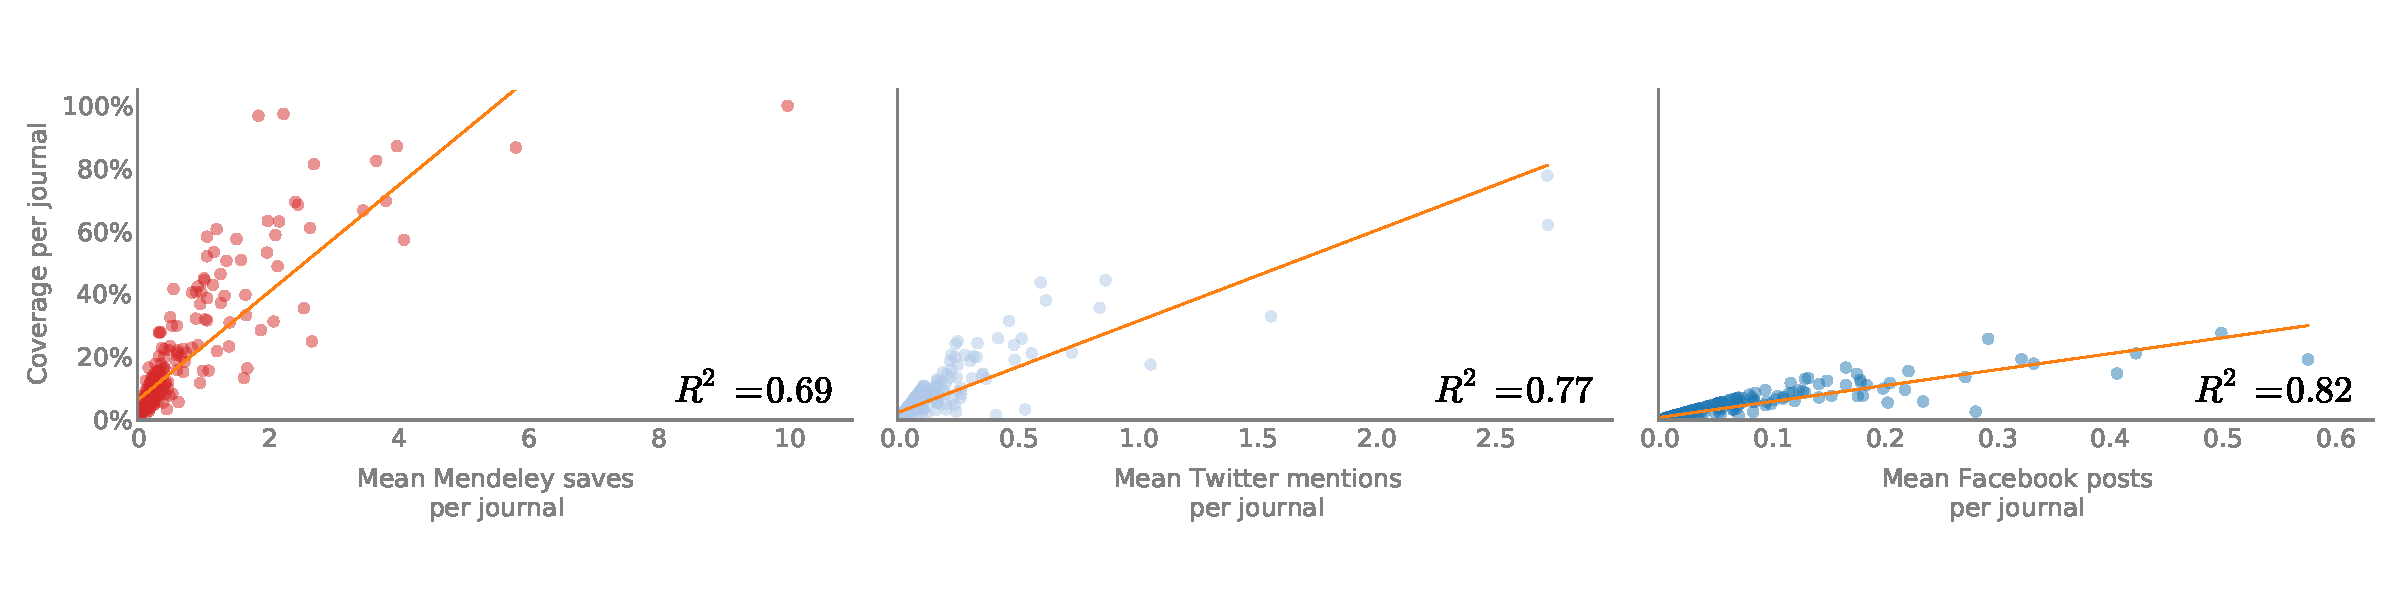
\includegraphics[keepaspectratio,width=\textwidth,height=0.75\textheight]{figures/altmetrics_coverage_v_mean_scielo_br.pdf}
\caption{Coverage of Main Metrics by Journal Compared to the Mean Value of Metric by Journal}
\label{altmetrics_coverage_v_mean_scielo_br}
\end{figure}

A key question in altmetrics work is the degree to which each of these metrics are measuring different signals of impact. As was discussed earlier, most altmetric studies to date show a low, but positive correlation between the various sources and citations. Unfortunately, the citation window in the SciELO Brazil dataset is too small to make similar comparisons to citations meaningful (there has not been sufficient time for citations to accumulate given that the altmetrics data is only available for articles published since 2013). In the absence of meaningful citation data, the top altmetrics were compared with the downloads counts of the full-text in the first 30 and 90 days after publication.

Mendeley, Tweets, Facebook, and number of full text downloads in the first 30 and 90 days since publication were all correlated using Spearman's rank correlation (\autoref{altmetrics_spearman_rank_scielo_br}). Twitter was the most highly correlated of the altmetrics, with coefficients around .2 with both the download metrics and with Facebook. No correlation was found between Twitter and Mendeley. The Spearman coefficients for Facebook were a little lower (around 0.15 with downloads in first 30 and 90 days) and, as already noted, .2 with Twitter. Again, no correlation was found between posts Facebook and Mendeley readers. Mendeley showed the lowest correlations across the board, with correlations of around .1 with downloads. The correlations, where they exist, are positive but low, similar to the effects found when comparing Tweets to citations (Haustein \& Peters, 2013). As can be expected from these low correlations, there is little overlap in the sets of articles that receive Tweets, Facebook posts, and Mendeley saves (\autoref{altmetrics_venn_scielo_br}).



\begin{table}[!htbp]
\centering
\begin{threeparttable}
\caption{Spearman Rank Correlation Between Mendeley, Twitter, and Facebook} \label{altmetrics_spearman_rank_scielo_br}
\begin{tabular}{@{}lccccc@{}}
\toprule
Metric  &   Twitter &   Facebook    &   Mendeley    &   \multicolumn{2}{c}{Downloads}   \\ \cmidrule{5-6}
        &           &           &           &(First 30 Days)    &   (First 90 Days) \\ \midrule
Twitter &   1   &   0.21**  &   0.03**  &   0.22**  &   0.2**   \\
Facebook    &   0.21**  &   1   &   0.01    &   0.15**  &   0.16**  \\
Mendeley    &   0.03**  &   0.01    &   1   &   0.11**  &   0.13**  \\
Downloads   \\
(First 30 Days) &   0.22**  &   0.15**  &   0.11**  &   1   &   0.84**  \\
Downloads   \\
(First 90 Days) &   0.2**   &   0.16**  &   0.13**  &   0.84**  &   1   \\ \bottomrule
\end{tabular}
\begin{tablenotes}
\small
\item **Correlation is significant at the 0.01 level (two---tailed)
\end{tablenotes}
\end{threeparttable}
\end{table}



\begin{figure}[htbp]
\centering
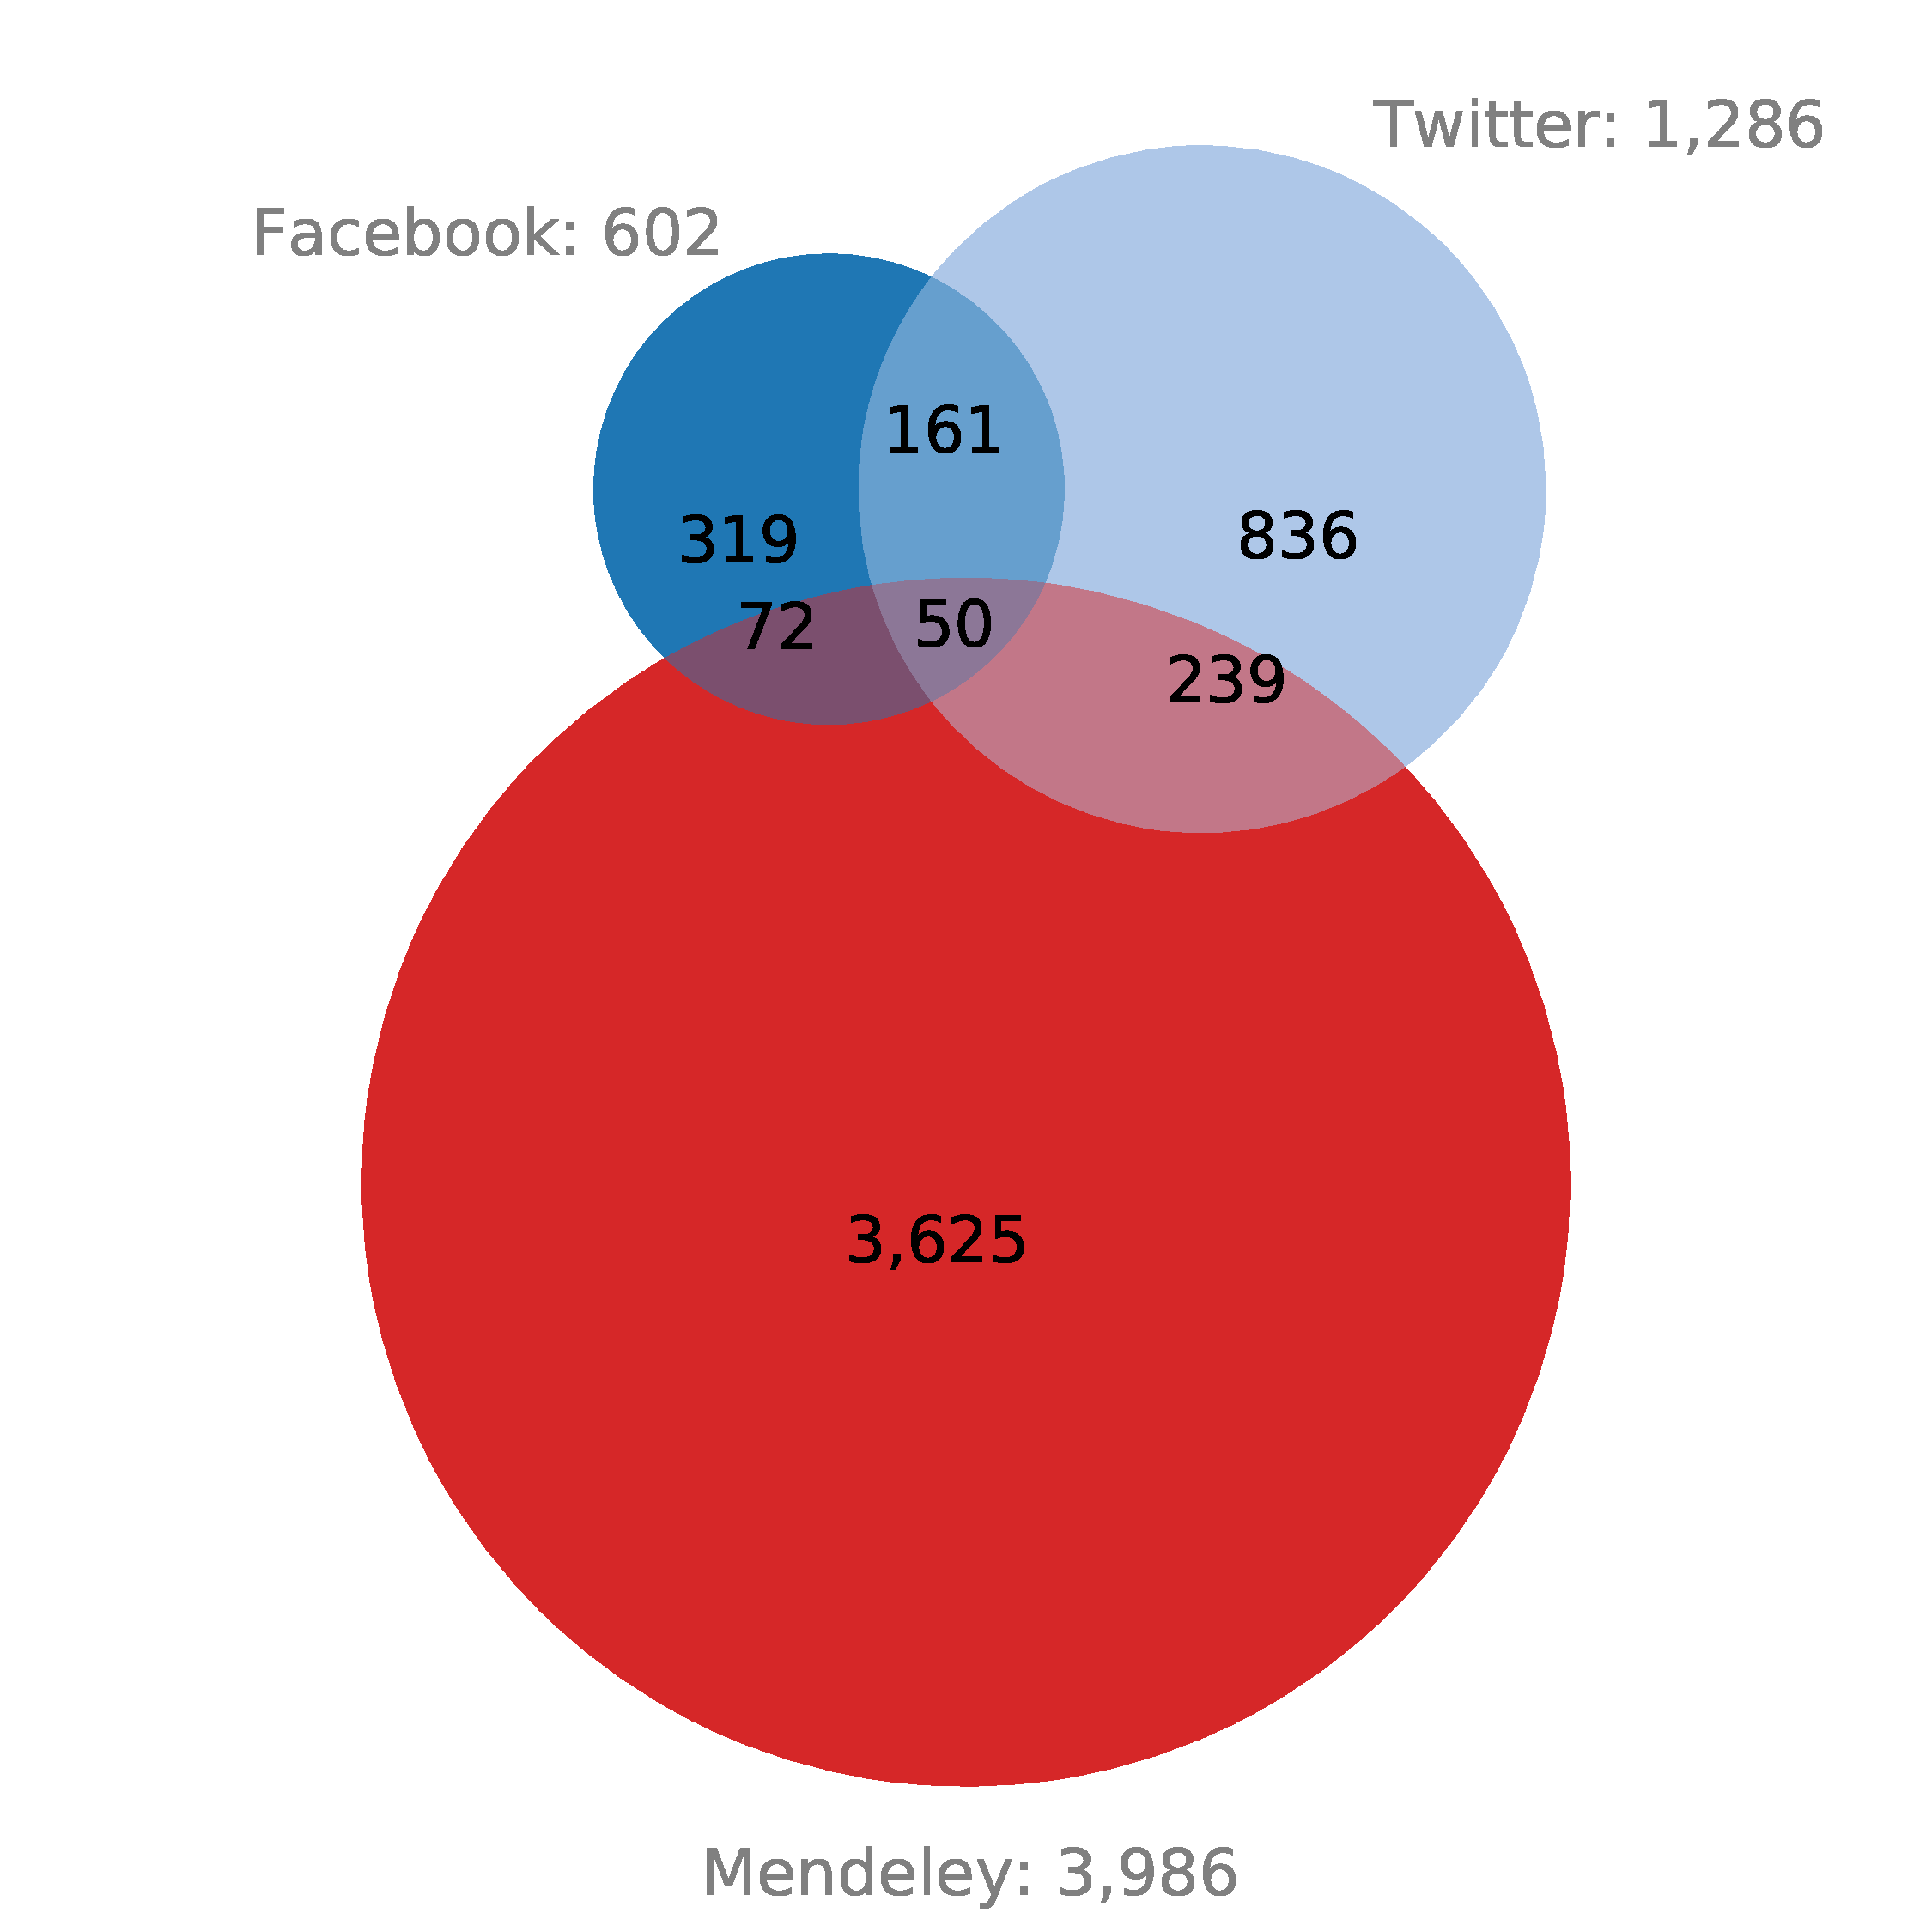
\includegraphics[keepaspectratio,width=\textwidth,height=0.45\textheight]{figures/altmetrics_venn_scielo_br.pdf}
\caption{Overlap of Altmetric Coverage of SciELO Brazil Articles for 2013}
\label{altmetrics_venn_scielo_br}
\end{figure}

Not only are the articles themselves different, but they are also comprised of different sets of languages, with coverage fluctuating depending on the language of the content. Content in English is about three times as likely to saved in Mendeley than content in Spanish or Portuguese (29.0\% of English content has Mendeley readers, versus 11.2 and 9.6\% of Spanish and Portuguese respectively). Content in Portuguese, however, is almost four times as likely to be shared on Facebook than content in Spanish, and almost twice as likely as content in English (3.8\% for Portuguese versus 1.0\% for Spanish and 1.7\% for English). It should be noted that, given that this data are drawn from the Brazilian journals in SciELO, the sample of Spanish articles is quite low (N=412 articles), compared to the dominant Portuguese (N=11,909) and popular English (N=8,850).

\autoref{altmetrics_coverage_by_subject} shows the coverage of these three sources is on articles of different disciplines. The Humanities Sciences, for example, have among the lowest Mendeley coverage, but the highest Facebook coverage and second highest Twitter coverage. The converse is true of the Biological Sciences, which have the highest levels of Mendeley coverage but amongst the lowest Facebook coverage. Engineering, on the other hand, has very low coverage on social media, but moderate coverage in Mendeley. The Medical Sciences seem to be the only field that is high across all three measures, with the highest or second highest coverage for each. These between field fluctuations in coverage levels are indicative of differing uses of social media, potentially indicating different audiences are being reached by each discipline or different practices regarding social media and reference management.

\begin{figure}[htbp]
\centering
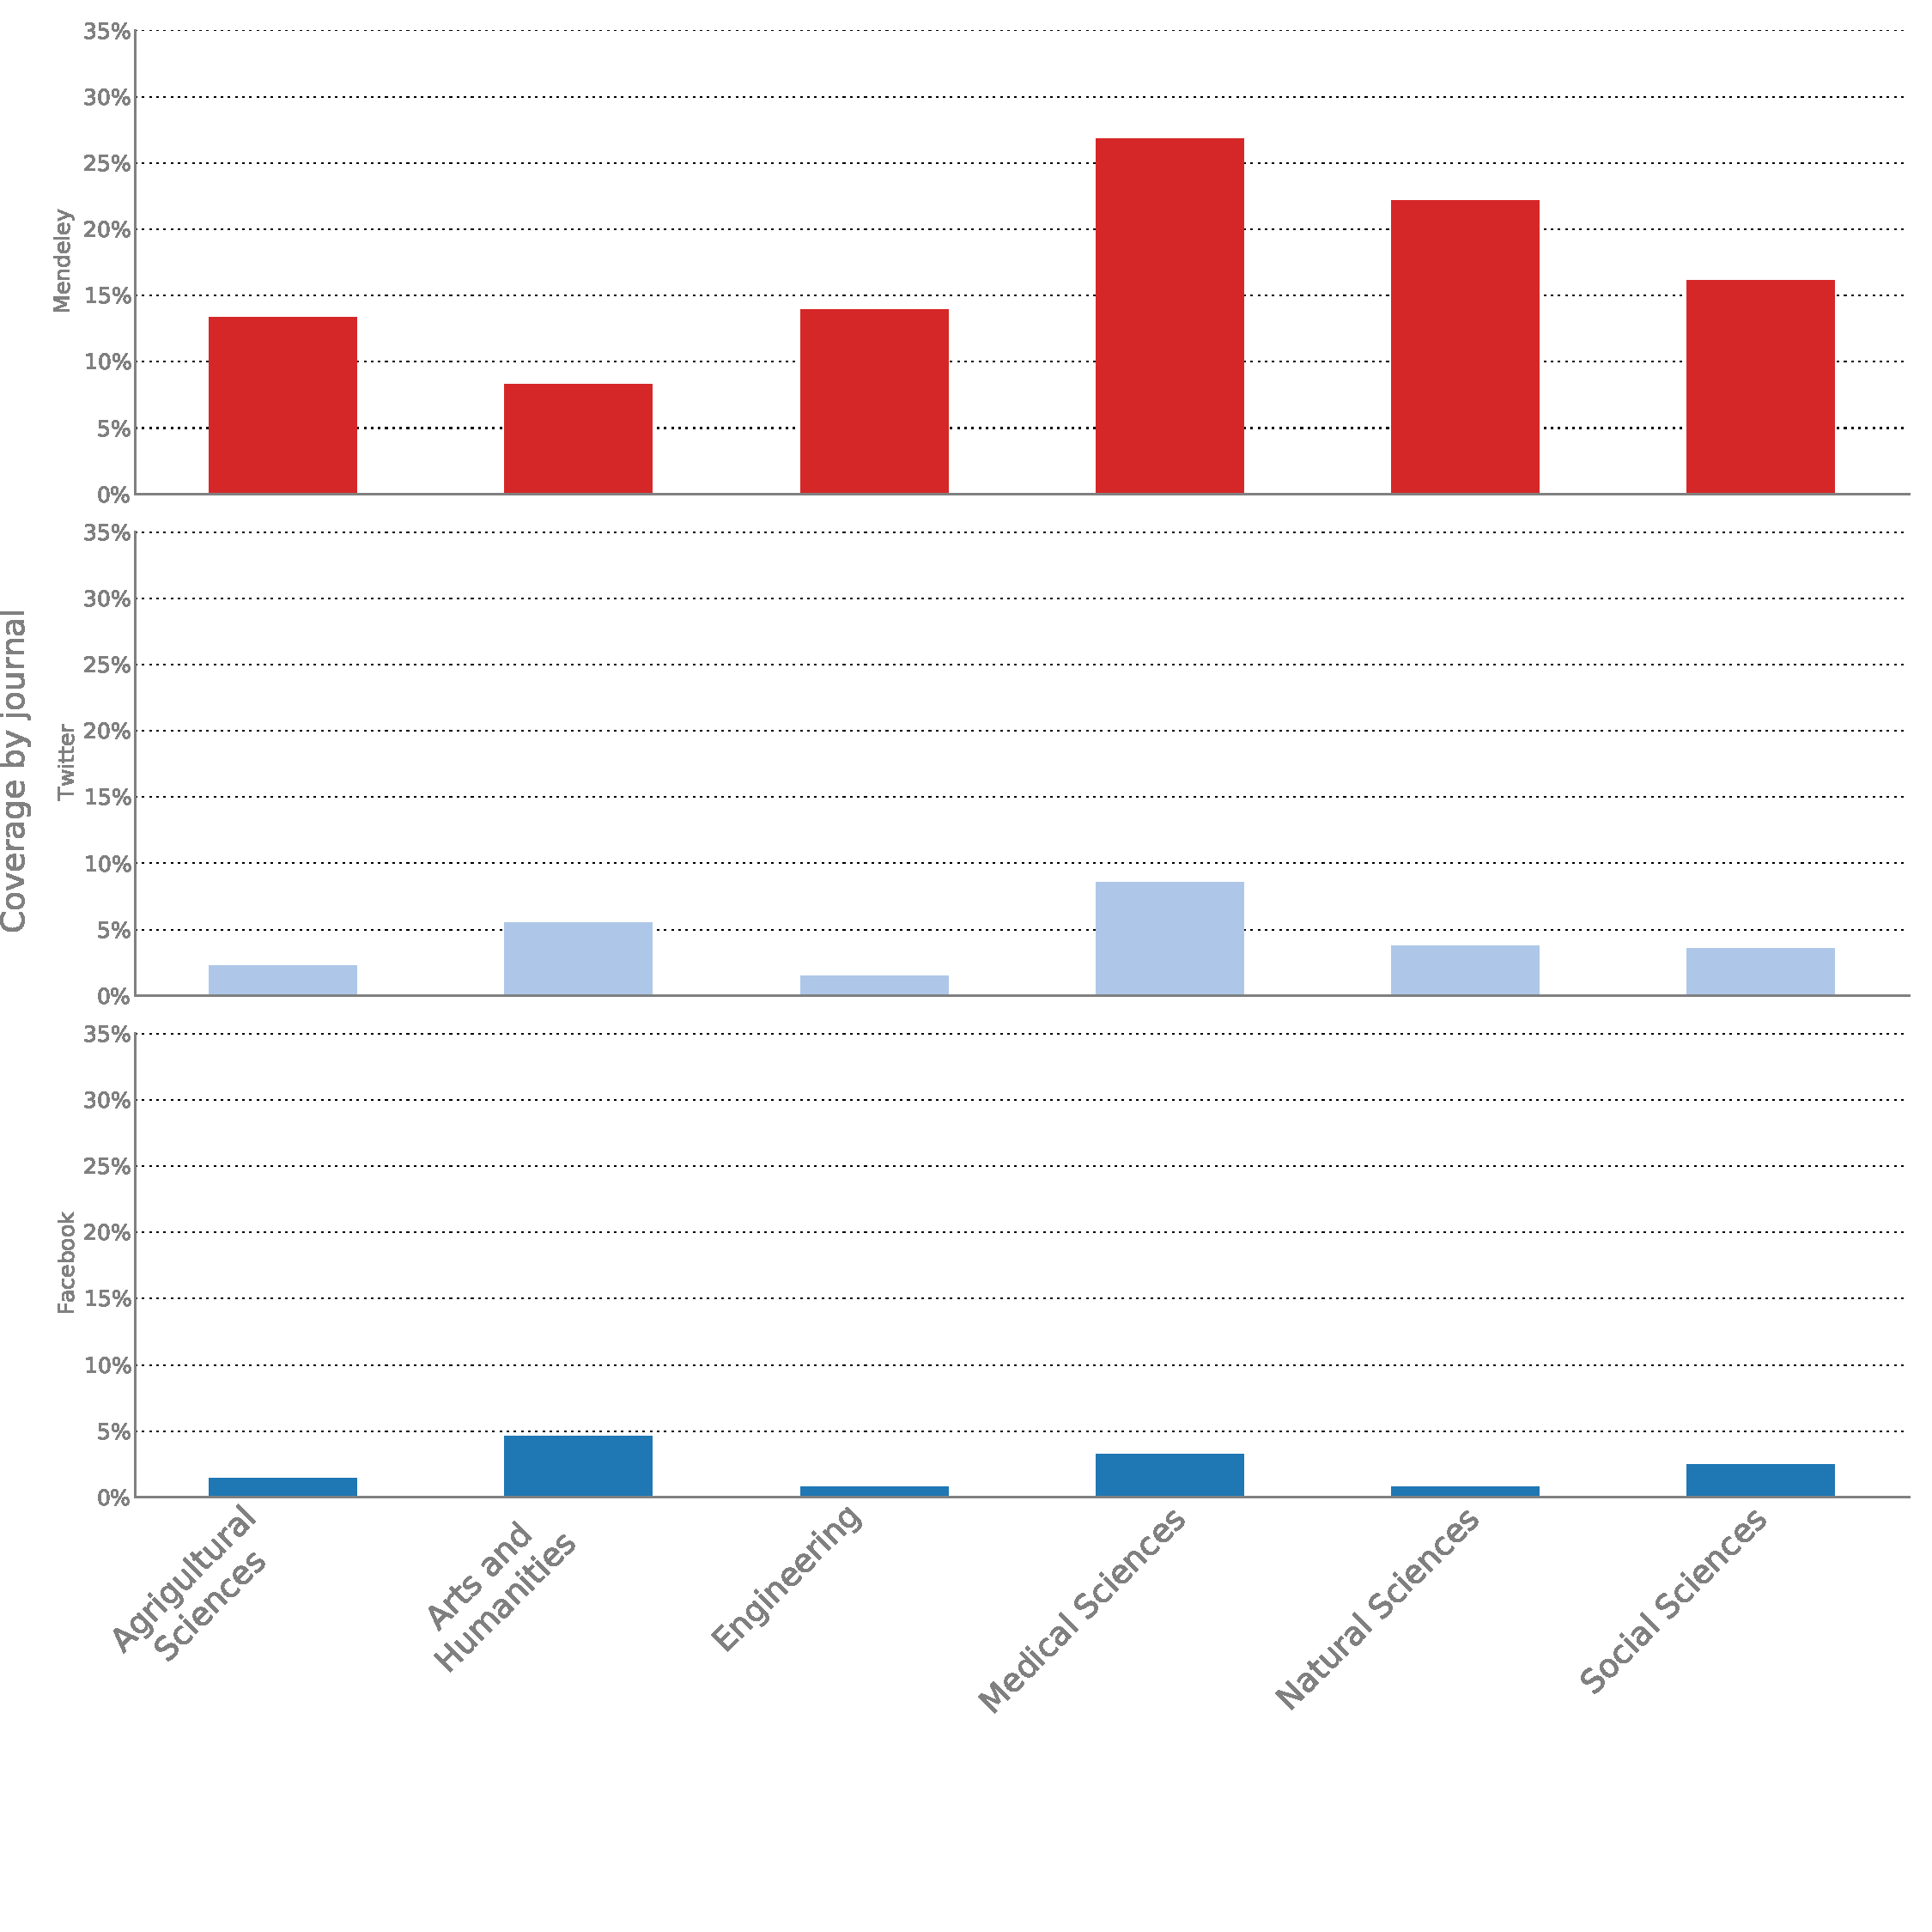
\includegraphics[keepaspectratio,width=\textwidth,height=0.45\textheight]{figures/altmetrics_coverage_by_subject.pdf}
\caption{Coverage of metrics by subject}
\label{altmetrics_coverage_by_subject}
\end{figure}

\subsection{Twitter Users}
\label{twitterusers}

The analysis above highlights that the Latin American articles published by SciELO and RedALyC do not yet have sufficient coverage on social media to conduct a wholesale analysis of the impact of all Latin American research. This should not be taken to imply that altmetrics cannot be used under certain circumstances to evaluate impact, nor that they will not be useful in the future as the prevalence of sharing articles on social media continues to increase. It also does not detract from the potential of altmetrics to capture forms of impact beyond citations.

To understand the type of impact that altmetrics may be useful in capturing, it is necessary to gain insight into who are the individuals who are sharing research articles on social media. The survey conducted over Twitter provides an initial glimpse into this population. Of the 286 respondents to the survey, 102 (36\%) reported not being affiliated with a university at all. Of the remaining 184 (64\%), 70 (24\%) report working for a university, 67 (23\%) report being students, while the remaining 47 (16\%) did not specify the nature of their affiliation \autoref{twitter_users_scielo_br_2013}.

The 36\% who were not affiliated with a university came from a very diverse set of backgrounds. Some came from the type of professions that you might expect would access research, like \href{https://twitter.com/MonikMazariegos/status/581559625964621824}{@MonikMazariegos}\footnote{\href{https://twitter.com/MonikMazariegos/status/581559625964621824}{https:/\slash twitter.com\slash MonikMazariegos\slash status\slash 581559625964621824}} who is part of the National Institute of Public Health in Mexico, , \href{https://twitter.com/darkgabi/status/579688882645676032}{@darkgabi}\footnote{\href{https://twitter.com/darkgabi/status/579688882645676032}{https:/\slash twitter.com\slash darkgabi\slash status\slash 579688882645676032}} who researches paleontology for her work at a museum, and \href{https://twitter.com/IanWoolf/status/580195651142565888}{@IanWoof}\footnote{\href{https://twitter.com/IanWoolf/status/580195651142565888}{https:/\slash twitter.com\slash IanWoolf\slash status\slash 580195651142565888}} who produces a science and technology podcast\slash community radio show. Several, were related to health, such as \href{https://twitter.com/JAJimenezOft/status/580041629643440129}{@JAJimenezOft}\footnote{\href{https://twitter.com/JAJimenezOft/status/580041629643440129}{https:/\slash twitter.com\slash JAJimenezOft\slash status\slash 580041629643440129}} (a doctor) and \href{https://twitter.com/asociacionsii/status/581443257181274112}{@asociacionsil}\footnote{\href{https://twitter.com/asociacionsii/status/581443257181274112}{https:/\slash twitter.com\slash asociacionsii\slash status\slash 581443257181274112}} (an association of individuals affected by irritable bowel syndrome). Others, however, came from a diverse group of professions, such as \href{https://twitter.com/eduardomps/status/582229360192688129}{@eduardomps}\footnote{\href{https://twitter.com/eduardomps/status/582229360192688129}{https:/\slash twitter.com\slash eduardomps\slash status\slash 582229360192688129}} who is a systems analyst, and \href{https://twitter.com/sonia_schoecher/status/580180389416812544}{@sonia\_schoecher}\footnote{\href{https://twitter.com/sonia\_schoecher/status/580180389416812544}{https:/\slash twitter.com\slash sonia\_schoecher\slash status\slash 580180389416812544}} who is a restauranteur. One individual, \href{https://twitter.com/ganaderiaLATIN/status/581547253229326336}{@ganaderiaLATIN}\footnote{\href{https://twitter.com/ganaderiaLATIN/status/581547253229326336}{https:/\slash twitter.com\slash ganaderiaLATIN\slash status\slash 581547253229326336}}, is an unemployed zootechnist who explains that she searches ``for information to advance her knowledge'' ~\citep[own translation]{ganaderiaLATIN2015}. These examples are not chosen randomly, but rather deliberately to demonstrate how the non-academic users run a full gamut of professions and interests.



\begin{table}[!htbp]
\centering
\caption{Type of Users who Tweeted SciELO Brazil Articles in 2013} \label{twitter_users_scielo_br_2013}
\begin{tabular}{@{}llcc@{}}
\toprule
                                        &               & \multicolumn{2}{c}{Respondents}                          \\
\multicolumn{2}{l}{Type of user}      & \multicolumn{1}{c}{Number} & \multicolumn{1}{c}{Percent} \\ \midrule
\multirow{3}{*}{University Affiliated$\left\{\vphantom{\begin{tabular}{c}3\\3\end{tabular}}\right.$}    & unspecified & 47                         & 16\%                        \\
                                        & employed    & 70                         & 24\%                        \\
                                        & student     & 67                         & 23\%                        \\
Not University Affiliated   &                       & 102                         & 36\%                        \\ \midrule
\multicolumn{2}{l}{Total}                               & 286                        & 100\%                      \\ \bottomrule
\end{tabular}
\end{table}


\subsection{Summary}
\label{summary}

Given the low levels of coverage overall, the altmetrics data serves a limited purpose. In the case of the journals in the RedALyC portal, the signal put out in social media is so low that it only serves to confirm that the only social networks being used by users of Latin American research are Twitter, Facebook, and Google+, although there is variability in the levels of use in social media among the journals of different countries.

The SciELO Brazil journals provide a better opportunity to study how research is shared. However, given that levels and patterns of use among social media users of research seem to vary between countries, any conclusions drawn from a sample drawn from a single country must be interpreted with caution. To start, the level of use is already much higher than all of the articles in the RedALyC portal, indicating both the higher levels of use of SciELO (as was seen in the previous section when analyzing downloads) but also higher levels of use of social media amongst its users. Even in the Brazilian case, however, coverage major sources like Twitter and Mendeley remain lower than what has been reported for other regions of the world ~\citep{Bar-ilan2014,Hammarfelt2014,Haustein2014a,Li2012a,Priem2012,Zahedi2014a}

As with other altmetrics research ~\citep{Haustein2014a,Shema2014}, we found low levels of correlations between the different sources, indicating that at article's presence in one media is not likely to indicate its presence in another. Mendeley is three times more prevalent than Twitter, which is in turn three times more prevalent than Facebook.

This coverage, however, varies significantly between sources and across languages and disciplines. The medical sciences, for example, are among the best represented in all sources (ranked first in Mendeley and Twitter and second on Facebook), but the Arts and Humanities are simultaneously the least popular on Mendeley and most popular on Facebook. Similarly, content in Portuguese is the least likely to be found in Mendeley, but most likely to be found on Facebook.

\chapter{Discussion}
\label{discussion}

The results presented in the previous chapter provide a clear answer to the main question posed in this study: \emph{do Latin American journals have impact and reach beyond the academic community?}. The answer: a resounding \emph{YES}. The pop-up and demographic survey results demonstrate that 16--25\% of the reach of the two Latin American journals portals is to non-university affiliated users and the Twitter survey demonstrates that 36\% of the impact of the research, as measured through its mention on social media, is also to a non-university affiliated public. These results are both surprising and significant in their own right, however, this study goes further by providing a more detailed understanding of the reach and impact of Latin American research and scholarship.

Although this study primarily sought to assess the public impact and reach, it used methods that allowed for the identification of alternative communities and other forms of impact. In doing so, it was possible to find that the research published in Latin America has impact and reach in at least two different communities, and therefore has two types of alternative impact: The first is \emph{public impact} as described above; and the second, a known but often overlooked type of impact, is \emph{pedagogical impact}, as seen through the use by students. Both the pop-up polls and demographic surveys confirm that two populations make up the vast majority of portal's use (as high as 80\%). I call these ``alternative'' in that neither group is made up of individuals who are themselves likely to be authors, and thus, all impact on these communities (public, pedagogic, or otherwise) would not have been detected in any citation-based (traditional impact) measure.

In seeking an answer to the main question of whether Latin American research has impact and reach beyond the academic community, three sub-questions were pursued, and can be condensed as follows: 1) who are those that access Latin American scholarly journals; 2) how do the different populations that access differ from one another; and 3) it is possible to identify these populations through publicly available data. While the first two speak directly to the main research question, the third explores methodologies that might be used to answer all these questions without the need to survey or poll users directly, as was done in this study.

This third question is answered later in the chapter through a discussion of the opportunities and limits of altmetric approaches to measuring impact. Similarly, the contributions, implications and significance of the findings, and the limits and strengths of the study itself are all addressed later in this chapter. However, this chapter begins by addressing the main and two first subquestions through a discussing of main findings—the discovery of the public and pedagogical impact of Latin American research. During these discussions, the results from the preceding chapter are situated in the existing conversations and literature of public and pedagogical impact.

\section{Public reach and impact}
\label{publicreachandimpact}

This study primarily sought to determine if Latin American journals had impact and reach beyond the academic community. Not only was it determined that they do, but that the public use of research from Latin America is significant. According to the pop-up and demographic survey responses, somewhere between 16--25\% of use comes from those not affiliated with universities.\footnote{The summary of the responses for both Q1 and Q2 for both portals can be found in \autoref{q1_summary} and \autoref{q2_summary}.} Unfortunately, however, I found no studies against which to compare this finding and say whether public use of Latin American research is higher than other regions. The Tenopir et al. studies cited earlier do explore types of readers, but do so with samples drawn only from within the university, and therefore do not provide a point of comparison regarding this non-academic reader population.

The presence of such levels of public use appear to be contrary to the common-place notion that academics as working primarily for each other, as inward looking, or as stuck in the heights of the ivory tower. Nicholas  \citet{Kristof2014} recently lamented the lack of public academics in the pages of the \emph{New York Times}, where he notes that ``to be a scholar is, often, to be irrelevant'' (n.p.). Kristof goes on to critique PhD programs for fostering ``a culture that glorifies arcane unintelligibility while disdaining impact and audience'' ~\citep[n.p]{Kristof2014}. Kristof's piece set of a spirited debate on academic's role in public life, which inspired no end of responses, debating the merit of Kristof's claim ~\citep{Daniels2014,Rothman2014,Chinn2014,Voeten2014} and inspired the Twitter hashtag \emph{\#engagedacademics} ``as if to refute Kristof's claim that professors don't use enough social media'' ~\citep[n.p.]{Rothman2014}.

However, none of these responses address the fact that academic's traditional acts of publishing in peer reviewed journals are engaging with the public to some degree—at least in Latin America. And they appear to do so, even though academic writing tends to use ``prose that is turgid, soggy, wooden, bloated, clumsy, obscure, unpleasant to read, and impossible to understand'' ~\citep[n.p.]{Pinker2014} or be ``knotty and strange, remote and insular, technical and specialized, forbidding and clannish'' ~\citep[n.p.]{Rothman2014}. The remarkable 16--25\% of the users who access the two portals used in this study are a testament of the public interest in the work being produced by academics. The fact that these portals, like much of Latin American research, is published in OA also reminds us that ``open access is also public access'' ~\citep[p. 111]{Willinsky2006}, and that the knowledge that goes into scholarly articles does not necessarily need to be translated for lay audiences or presented in other venues for it to reach beyond the walls universities. The pop-up surveys demonstrate the extent of this reach in a context like Latin America, where so much research is publicly available through OA portals.

That said, Latin America is not the only region of the world in which interest in scholarly articles by non-academics has been registered. The National Institute of Health in the United States, for example, has had a public access policy in place since 2008, a policy that ensures that all research funded by the agency is made publicly available within twelve months of publication.\footnote{http:\slash \slash publicaccess.nih.gov\slash } After a directive from the Obama administration in 2013, many other US funding agencies are following suit, including the National Science Foundation (the largest funder of research in the country). Such policy advances obviously speak to the public policy implications of these findings, something I return to later in the chapter. The early adoption of a public access policy from the health funding agency is indicative of the perceived importance of access to health related research by health personnel and to the public at large.

In the case of the Latin American portals studied here, the public relevance of the health-related research beyond the academy is evident by looking at both the pop-up survey results and the topic models. The breakdown by discipline from pop-up survey results (summarized in \autoref{scielo_q1_q2_by_latindex_subjects} and \autoref{redalyc_q1_q2_by_latindex_subjects}) shows that articles classified as Medical Sciences are of interest to those accessing for professional practice reasons more than any other discipline. This is evident in the case of SciELO, where 20\% of all downloads medical science articles downloaded, were downloaded by those researching for professional practice reasons, and where medical science articles received, on average, the highest number of downloads.

This extra attention health articles received from the professional community is especially noticeable in the answer to Q1, and still present in the answer to Q2. The interest in health can also been seen through the topic models created from the titles of the papers downloaded by those with professional interests in the research. As was pointed out earlier, the top terms associated with public and non-profit sector respondents are dominated by health-related terms, indicative that the majority of papers downloaded by people in those categories were on health-related topics (\autoref{top20_terms_q1}). These two sectors, public and non-profit, are consistent with the sectors that are home to the primary institutions in which health professionals can be found: hospitals and clinics.

Professionals from the public and non-profit sectors, it seems, are interested in health research. Such an interest by health professionals in primary research is also not unique to Latin America. In a survey of 90 health professionals from small clinics in Northern California,  \citet{OKeeffe2011} found that 30\% of health personnel surveyed reported accessing research articles on a regular basis. In another study, this time conducted at the Stanford University Hospital,  \citet{Maggio2013} also found that health personnel made use of primary (and secondary) literature. The results presented here indicate that Latin America is no different, and even suggests that Latin American research may have an even larger public impact.

As extensive as the public use from health research on professional practice is, it is just one of the forms of public use uncovered by this study. Health topics were also dominant among the ``personal interest'' users of both portals, showing the use of health research goes beyond the professional sphere and reaches the general public. This is consistent with individuals searching because of personal health concerns (i.e., to understand a diagnosis, or to investigate treatment options, or look up drug side effects), although no specific topics or rationale were studied.

Personal interest in research also extended to all other disciplines. The comparisons of the topic models shown above (\autoref{llda_cosine_similarity_q1} and \autoref{llda_cosine_similarity_q2}) indicate that those accessing for personal interest are reading topics most similar to those affiliated with the university—a wide spectrum of topics across all disciplines. This group of users is not negligible. On the whole, those researching for personal interest made up 7.9 and 10.5\% of all respondents to Q1 for RedALyC and SciELO respectively (\autoref{q1_summary}), while those researching for personal reasons (Q2) made up 5.9 and 7.9\% for RedALyC and SciELO respectively (\autoref{q2_summary}). Again, a remarkable level of public use by individuals accessing for personal interest and gain, and the potential impact that this literature has on the non-academic public.

In contrast, the topic models indicate that the downloads from those interested for their work in the private sector have a very different topic profile, with top terms loaded on words related to research methods, as described in the previous chapter (\autoref{top20_terms_q1}). All this suggests, as with the pop-up surveys themselves, that the audiences of Latin American research are quite varied. Not only do they come from different sectors and with different motivations, but they access different content and likely need a broader range of indicators of impact than citation-based measures.

Overall, the results presented in the preceding chapter point to the measurable public use of research published in Latin American for both professional practice and for personal use. The use of health-related research is primary among the disciplines, but this use is not limited to the one subject field. Furthermore, each of the sectors have a unique topic profile, indicating that each is accessing with unique information needs. On the whole, the results presented show that the research reaches non-academic audiences at a significant scale.

Furthermore, there is evidence of a sizable proportion of those sharing articles on social media (Twitter in particular) being non-academics (\autoref{twitter_users_scielo_br_2013}). In the small survey conducted of Twitter users who had shared an article from SciELO Brazil, 36\% of respondents were not affiliated with a university. The coverage of articles on social media by discipline described in \autoref{altmetrics_coverage_by_subject} once again points to the importance of health-related research, as it makes up a highest proportion of articles shared on Twitter, and the second highest proportion of posts on Facebook (only one percentage point behind the humanities). While the overall proportion of articles shared on different social media was generally low, the high proportion of these shares from non-academics is still clear evidence of the public impact of the research. That is, even if (as is discussed in a subsequent section) only a small portion of the impact can currently be captured by social media metrics because of low coverage levels, the proportion of the impact is rather high. There is therefore no doubt that there is some public impact, but it is an open question whether or not the proportion of public impact captured from Twitter users (36\%) would remain constant if overall mentions across the Web were higher.

Before delving into the extent to which impact across social media could be used as a measure of impact for Latin American research, the next section highlights the second alternative community for which this study uncovered alternative impact and reach—students.

\section{Pedagogical reach and impact}
\label{pedagogicalreachandimpact}

The number of students using Latin American research is even higher than the public use described above. According to the pop-up surveys (Q3), students make up 65 and 55\% of the users of RedALyC and SciELO respectively (\autoref{q3_summary}). These numbers change slightly when looking at the demographic survey, in which students make up 47 and 42\% respectively (\autoref{demographic_parallel_coordinates_redalyc} and \autoref{demographic_parallel_coordinates_scielo}). Despite this discrepancy between the percentage reported by each instrument, both portals have similar student-staff ratios, which are the reverse of what has been reported by  \citet{Tenopir2000}, who estimated that up to one third of journal readership (based on a sample of only readers from within universities) were themselves not authors (i.e., students). In the Latin American portals, we see inverted proportions, where two thirds of the university-affiliated users are students, and only one third are faculty or staff (\autoref{demographic_parallel_coordinates_redalyc} and \autoref{demographic_parallel_coordinates_scielo}).

This further strengthens the hypothesis that one of the largest forms of yet-unmeasured impact of Latin American research may be pedagogical impact, as the research contributes to the student's educational materials and forms part of their educational experience ~\citep{Evans2013}.  \citet{Evans2013} speak to the pedagogical advantages of having students access research in its ``native'' environment (as opposed to through course-pack readers), citing the presence of ``links to the article's references'' and the serendipitous discovery enabled by being only ``a click away from the table of contents for the journal'' (p. 350). This study did not seek to uncover this type of impact, but it did uncover that the research published by the Latin American portals has significant reach among students, paving the way for the kind of scenarios envisioned by  \citet{Evans2013}.

This kind of reach also has another potential consequence. As students read the research available through these portals, they could learn through exposure what constitutes scholarly research and of how scholarly research should be written and presented. Again, this study sought did not seek to measure or study any learning outcomes of students, but in uncovering the extensive reach of Latin American research to students, it found that students are at the very least exposed to numerous examples of the research writing type (genre). As such, it is conceivable that students are learning the ``conventions of particular text types and disciplines'' that  \citet{Curry2005} suggest ``may be best demonstrated using example texts'' (p. 24).

If the students accessing the research are themselves from Latin America (something that seems likely, but that this study did not confirm), a reasonable hypothesis would be that students are using these portals in such high proportions because the content is not only open access, it is also written primarily in their native languages (Spanish and Portuguese). However, the evidence to support this hypothesis is somewhat murky, partially due to the research design. As pointed out earlier, the responses to Q1 that separate out students from other academic roles are confounded by the double meaning of the phrase ``my work at a university'' in both Spanish and Portuguese, which some students interpreted to mean ``my assignment for a class at the university.'' Responses to Q3, the only survey question that can be used to clearly distinguish between students and others at the university, itself provided only partial evidence.

The native-language hypothesis is in part supported by the responses to both portals, where a higher proportion of the Spanish and Portuguese content was accessed by students than of the English content (\autoref{redalyc_q1_q2_by_original_language} and \autoref{scielo_q1_q2_by_original_language}). However, in the case of RedALyC, the Portuguese content was accessed by only a fraction more than the English content (in both cases, students were responsible for \ensuremath{\sim}60\% of all responses). Spanish content was accessed by a larger proportion of students (\ensuremath{\sim}65\%). In both portals, English content was accessed most by university employees than any other group, again consistent with the hypothesis that students access content in their native language, while staff are the group that makes the most use of English-language content.

Despite this difference between portals, there are strong similarities between the topics that the students and university staff are accessing on the whole. The comparison of topic models for the Q1 answers show that the two groups of users whose topics are most similar to one another (\autoref{llda_cosine_similarity_q1}). One possible explanation is that these groups are accessing papers with similar topics because of a relationship between professor's research interests and the topics of the classes they teach (and hence what the students are researching about). Unfortunately, the data collected was not sufficiently detailed to know the goings-on in the classroom or to know if this type of use was taking place. This situation would also be consistent with faculty bringing research into the classroom, or asking undergraduates to do research themselves, which is known to produce ``several documented educational benefits'' ~\citep[p. 190]{Designs2007}. While these ``benefits of research normally reach only a limited subset of the student body'' ~\citep[p. 190]{Designs2007}, they would nonetheless be considered pedagogical impact.

The degree to which this may be going on is unknown, and the impact it may have on teaching becomes even murkier when taken in the context of the demographic survey results which suggest that the majority of the university population does not hold a PhD (only around 30\% of users who are university staff hold a PhD) (\autoref{demographic_work_education_pivot_redalyc} and \autoref{demographic_work_education_pivot_scielo}).\footnote{This is not to say that those reading Latin American research are not highly educated. The majority of the users (\ensuremath{\sim}75\%) are at least partially university educated (\autoref{demographic_parallel_coordinates_scielo} and \autoref{demographic_parallel_coordinates_redalyc}).} The language difference mentioned above does imply some differentiation between the research accessed by the two groups, presumably indicative of more experience in researching in the \emph{lingua franca} of academia (English). However, the lack of formal research training by most of the academic users of the portals suggests that both populations could be learning from these examples of research while under increasing pressures to produce research outputs.\footnote{In the case of Brazil, the Latin American country where this pressure is perhaps most acutely felt, ``graduate programs are ranked in terms of their research productivity and financed accordingly'' ~\citep[p. xvii]{Altbach2009a}.} This combination means academic staff, especially those who may not have been on a research track previously, are likely on the lookout for a model of research to follow, and the open access papers available to them through SciELO and RedALyC provide such a model. This may be yet another way in which the research is influencing aspiring scholars that has gone largely unmeasured to date.

The pedagogical impact described above has been speculative, stemming from the large reach among students measured in this study. However, this study also uncovered one concrete measure of impact on the student population (although not necessarily pedagogical impact) through the survey of Twitter users who had shared an article from SciELO Brazil. This survey revealed that 24\% of those Tweeting research articles were university-affiliated students. As a proportion of users, this number is significantly lower than the \ensuremath{\sim}50\% students who access both portals (although the 16\% unspecified academic use should also be taken into consideration). As with public impact, the potential of altmetrics for capturing impact on students may be limited because of low coverage levels, and doubly so because of the relatively low proportion of students who are part of those who share articles on social media. Despite this limitation, this study can confirm that some students are interested in sharing research on social media channels. In this light, 24\% of those Tweeting is a remarkable percentage, and clear evidence of impact that is not measurable through traditional citation-based measures.

These findings suggest that the impact of Latin American publications, however big or small it may be, is decidedly different from the traditional notion of impact as defined by citation metrics. As was laid out at the beginning of this chapter, up to 80\% of the users of the portals, whether they be students or public users, is ``alternative.'' That is, it is by users who are themselves not likely to be authors that may eventually cite the works they are reading. In this light, it is imperative to uncover methods to capture, measure, or simply identify alternative reach and impact of Latin American research.

\section{Measuring alternative impact}
\label{measuringalternativeimpact}

For this reason, the third of the dissertation sub-questions was posed to determine to which extent it possible to use publicly available data to systematically measure the impact of research on both the academic and public audiences. The short answer is that neither the download nor the altmetric data are particularly useful at this point in time. The download data, at the level of granularity studied here, did not present a clear distinction between the public, student, or academic sectors. The altmetric data, suffered from a different limitation: coverage levels were inadequate to speak to the the research published in the portals as a whole.\footnote{Portions of this section have been previously published in  \citet{Alperin2015b}.}

This study looked at ways of measuring both reach and impact of this work, first with downloads and second with altmetrics. The exploration of download counts across disciplines and across response types, however, did not yield terribly useful results for new ways of differentiating between traditional and alternative reach. Downloads are, for the most part, not significantly different across subjects (\autoref{downloads90_by_subject_redalyc} and \autoref{downloads90_by_subject_scielo}) or across survey answers by respondents (\autoref{downloads90_by_q1_q2_redalyc} and \autoref{downloads90_by_q1_q2_scielo}). The only notable exception are the medical science articles from Brazil, which do have higher average download counts than other disciplines. This overall similarity still suggests that the articles read by the public, students, and staff are either being consumed in similar volumes, or the groups are reading across the same set of articles. Either way, their download counts are interspersed and indistinguishable at this coarse level.

This high-level analysis of download counts should not be interpreted to mean that download counts could not be helpful in distinguishing alternative impact of research. Despite the lack of clear way of capturing, measuring or identifying alternative impact from download counts, the pop-up survey results summarized in \autoref{q1_summary}, \autoref{q3_summary}, and \autoref{q3_summary} clearly show that these alternative communities do download articles from these portals, so it may still be possible to use download data in some way to capture the use and impact on these communities.

Full download data would have two useful characteristics that could not be exploited in study, but which may prove useful in future research. The first, is that there are metrics for nearly every published article (unlike altmetrics, as I return to shortly). The second is that there is time-series information that may show different patterns between groups of users over time. However, as described in the preceding chapter, at the time of data collection, both RedALyC and SciELO only made download data for articles published in 2013 available, thereby limiting both the data that could be linked to survey responses to only a small subset, and simultaneously restricting the time window over which which trends could be observed.

The potential of altmetrics was similarly explored, although similar conclusions were reached: there is a clear indication that all users communities are represented in the altmetrics data, but there is yet no clear way to identify the different communities from the data alone. Meanwhile, altmetrics continue to receive attention among the scholarly communication community as a potential for uncovering various forms of impact beyond citations ~\citep{Torres-Salinas2013,Costas2014,Haustein2013,Eysenbach2011,Bollen2008a,Bollen2009}.

While both the public and student communities are present in the altmetrics data, at least on Twitter (\autoref{twitter_users_scielo_br_2013}), the levels of coverage by the major altmetrics sources is quite low (\autoref{altmetrics_coverage_by_subject}), making the use of altmetrics data problematic for any systematic analysis. Moreover, using altmetrics in the Latin American contexts are doubly problematic because the levels of coverage are generally lower than what has been previously reported elsewhere. Most sources showed zero or almost zero coverage for all of the RedALyC and SciELO collections. In the case of SciELO Brazil, which was studied in more detail, large differences were found even among the metrics that showed the most coverage (Mendeley, Twitter, and Facebook).

Of these, the most dramatic differences were found for Twitter, for which ~\citep{Haustein2014b} found that over 20\% of articles from 2012 were tweeted at least once (twice that of 2011) using a set of articles in both PubMed and WoS. Other Twitter studies have found that 39\% of arXiv papers (from 2012) are tweeted at least once ~\citep{Haustein2014a} and over 11\% in an older study of PLOS One articles (from 2010) ~\citep{Priem2012}. Again, the study showing the lowest coverage was  \citet{Zahedi2014}, who found only 4\% of 2011 papers had Tweets (a doubling from 2010 and a quadrupling from 2009). However, the trend identified by both  \citet{Haustein2014b} and  \citet{Zahedi2014} suggests that by 2013 similar samples would have even higher coverage in 2013, in both cases eclipsing the 6\% found for the 2013 articles from SciELO Brazil.

For Mendeley, the differences are especially pronounced for the most recent year. The lowest reported coverage in Mendeley (for articles in the most recent year) was 57\%  \citet{Zahedi2014} followed closely by another at 61\% ~\citep{Hammarfelt2014}. The first of these studies is derived from a random sample chosen from the WoS (from 2011) and the second from a small sample of articles from a Swedish University. For studies that include Mendeley, 60\% is in itself a low figure given that most studies report values of over 80\% (and some as high as 95\%) ~\citep{Li2012a,Priem2012,Bar-ilan2014,Zahedi2014a}. These levels of coverage dwarf the 19\% found for SciELO Brazil in 2013, although they are closer to the coverage levels when looking at articles from more than two years prior. The reported values suggest that SciELO Mendeley coverage may approach that found elsewhere, although there appears to be a longer lag in articles being saved into the reference manager (of approximately two years).

The gap between the Facebook coverage of SciELO Brazil and that of previous studies is not as clear. While  \citet{Priem2012} found a quarter of 2010 PLOS One articles to be shared on Facebook, as few as 2.8\% of the 2013 SciELO Brazil articles were mentioned on the platform. This appears to be a significant different, but a direct comparison is hampered by Altmetric.com's method of querying Facebook, which captures only public posts whereas the method used by  \citet{Priem2012} captures all posts. As a result, Altmetric's method misses a potentially large segment of all links shared on Facebook. The 2.8\% of SciELO articles found on Facebook is consistent with the coverage levels found by  \citet{Hammarfelt2014} using Altmetric's data for the small Swedish University sample.

Overall this speaks to the generally lower levels of coverage, especially for the two most prevalent sources (Mendeley and Twitter), and therefore lower potential for altmetrics to serve as a valuable tool to capture, measure, or identify alternative impact in Latin America. There are at least three plausible explanations for this lower coverage: 1) the articles published in SciELO simply have lower usage overall, and this is reflected in lower social media usage; 2) the levels of social media usage, at least among academics, is lower in Latin America than in the previously studied contexts; or 3) there is a different culture surrounding the sharing of research on social media among the readers of Latin American research. Each of these possible explanations warrants further investigation.

To complicate matters further, the results also show that the coverage varies by field and by metric, and with it the potential of altmetrics for measuring impact, especially when one takes into consideration the disciplinary differences uncovered between each group of users. Such disciplinary differences in various social media metrics have been studied in other contexts, with similar notes of caution noted about the interpretation and use of the metrics across subject fields ~\citep{Holmberg2014,Costas2014}. However, the lower levels of coverage in combination with the variability across subjects must be accounted for.

On what may be seen as an encouraging sign, the low correlations between downloads and any of the social media metrics (\autoref{altmetrics_spearman_rank_scielo_br}) is indicative of the complementary nature of downloads and altmetrics. While other studies have already confirmed a similar relationship in relation to citations ~\citep{Torres-Salinas2013,Costas2014,Haustein2013,Haustein2014b,Eysenbach2011} and yet other studies have shown the complementary nature of citations and downloads ~\citep{Bollen2008a,Bollen2009}, this study confirms that altmetrics capture impact through social media that is somehow different than what is captured by looking at the popularity of articles through downloads. Each metric measures a different form of impact or reach, which means that altmetrics may indeed have a role to play in measuring the impact on non-authoring populations such as students and the general public.

Despite the limits of altmetrics highlighted here, they must be considered in the context of a situation that is changing rapidly and that will be worth returning to. The sharing of research articles on social media appears to be highly variable, making the analysis of trends over time necessary for making sense of what altmetrics have to offer. What the Twitter survey makes clear, however, is that students, academics, and non-academics are all sharing articles on social media (\autoref{twitter_users_scielo_br_2013}). Although coverage levels are generally low today, they are still capturing a portion of the public and pedagogical impact highlighted, and as such are a demonstration of the potential of such metrics.

\section{Contributions and implications of findings}
\label{contributionsandimplicationsoffindings}

This study has made several concrete contributions with conceptual and methodological implications. This section will outline the contributions of this study as a whole, and delve further into the implications of the main findings outlined in the first part of this chapter.

At the forefront of these contributions is the documentation of the alternative impact of Latin American research. This contribution—the main finding of this study—is in itself significant for understanding scholarly communications in Latin America. As was outlined in the latter part of Chapter 2, there is a dearth of research on the impact and reach of Latin American scholarship; this study is among the first to provide concrete measures of both of these dimensions, and does so at a time of increased attention on the region's research universities and research outputs ~\citep{Altbach2007,Bernasconi2007,Altbach2013}. As  \citet{Altbach2013} reminds us, ``understanding the characteristics of the research university and building the infrastructures and the intellectual environment needed for successful research universities is a top priority'' (p. 329). While  \citet{Altbach2013} speaks of the characteristics of the universities themselves and the university system as a whole, it is logical to extend his sense of urgency for understanding the characteristics to scholarly outputs and the scholarly communication system as well.

There has already been palpable sense of urgency felt from within the region in understanding its own research outputs. However, over the last several years, the emphasis has been on studying the production of journals and attempting to measure quality. The very fact that three of the most successful initiatives in the region (Latindex, SciELO, and RedALyC) have primarily focused on producing indicators of editorial standards, growth, and authorship ~\citep{Alperin2014c} is in itself revealing, as are the numerous studies on the subject, including nine reports published by RedALyC's own research laboratory ~\citep{RedALyCFractal} and many others, including ~\citep{Cetto1998,Collazo-Reyes2008,Alonso-Gamboa2012,Russell1998,Russell2009}.\footnote{As was discussed in Chapter 2, the exception here is SciELO, which has produced citation indicators since its inception (and even calculates an Impact Factor for its journals). Very few studies have actually sought to study Latin America's citation impact with this data ~\citep[among a handful of others]{Pereira2006,Pinto2007,Huamani2009,Meneghini2006,Luna-Morales2007,Packer2007}, as well as a few others that have done so with data from other bibliographic databases that severely underrepresent and mischaracterize the impact of the region's research.} It has only been in the last year that RedALyC and SciELO have begun to make download data available to the public, and this is the first study to take advantage of this data.

The time is right, after more than a decade of operation of these three initiatives, to move beyond looking at \emph{what} is published, and to begin to understand its impact and reach. Under this belief, this study does not just seek to fill an existing gap in the existing research, it is hoped that it will also usher a new era of research on Latin American scholarly communications that focuses on these two dimensions.

This study also goes beyond exploring the impact of the research, it also contributes to our understanding of the value that the public finds in having access, in a world that has been increasingly moving towards providing such access through different open access models. Although this study cannot speak to the effects of OA directly (that is, it cannot be said that open access is the cause of the type of public and pedagogical impact uncovered), open access did facilitate the public's access in the Latin American case (specifically through the OA portals studied). This study therefore expands our understanding of the potential value that the public finds in open access, even though it might have found equivalent or greater value if given access through other means.

In this way, this study does speak to the growing literature that seeks to explore the implications of OA, despite not directly building a case about the effects of OA (which were not studied or established through a comparison to closed-access literature). Other works have made arguments about the benefits of OA in a number of ways, including (but not limited to): a citation advantage (i.e., OA will lead to increased citations); an ethical imperative (i.e., it is the right thing to do); an economic necessity (i.e., to ease the financial burden on university budgets from subscriptions); a responsibility to the tax-payer (i.e., the tax-payer is entitled to tax-funded research); an acceleration discovery imperative (i.e., easy access and few re-use restrictions leads to faster science); a contribution to development (i.e., to bridge an access to knowledge divide); as well as two additional premises that are most germane to this study: the educational benefit of informed teachers and students, and the public enrichment enabled by public access.\footnote{Of these, perhaps the most widely researched and controversial has been the citation advantage, for which it is possible to find an entire bibliography ~\citep{Hitchcock2013}.}

To date (and despite being almost a decade old), Willinsky's (2006) book, \emph{The Access Principle: The case for open access to research and scholarship}, is one of the most complete and compelling justifications for OA. In it, Willinsky argues (among other things) for the public value of OA, but readily admits that ``the common reader's downloading of the latest article on trilobites from the Journal of Paleontology is unlikely to be the number-one argument in convincing researchers'' ~\citep[p. 125]{Willinsky2006}. While this study found no downloads of trilobite research by people interested for personal reasons, it did uncover personal interest in titles such as: ``One-Pot Synthesis of 1,8-Dioxodecahydroacridines and Polyhydroquinoline using 1,3-Di (bromo or chloro)--5,5-Dimethylhydantoin as a Novel and Green Catalyst under Solvent-Free Conditions'' and ``Petrography and mineral chemistry of Escalón meteorite, an H4 chondrite, Mexico.'' That is, the personal interest category spans much further than what might be commonly thought. And even though Willinsky is right that it may not be the number-one reason, the personal interest category of readers is not insignificant, at 6--11\% of the portal's total use.

In many of the discussions regarding public access, the medical sciences are the emblematic example, for obvious reasons. It is easy to understand and explain why the general public (i.e., patients) and professionals (i.e., doctors and other health professionals) might be the most interested in accessing the latest medical research. This study supports this rationale—the medical sciences do appear to be the most sought after field by non-academics—but it also demonstrates that the public is interested in much more than just medical research.

In short, the findings in this study provide a direct response to Willinsky's (2006) assertion that ``it is hard to determine in advance what the public will make of the growing access to all fields of scholarly endeavor'' (p. 125). As the Latin American case shows us, there is evidence of a latent interest among the public in accessing research across all fields, and that interest indicates a greater potential readership than has previously been possible, at least a context where there are no financial barriers for the public to gain access.

The apparent interest by the public in accessing research uncovered by this study points to the need to better understand how the public will benefit from receiving access. Again, while this study did not study the effects of open access, the clear indications of the public's interest in accessing the primary literature point to a need for further research that specifically looks at the effects of different approaches to provide this access (including, but not limited to open access). Yet, too often, the potential value of public and open access approaches on the public take a backseat to the effects within the academy itself. This may be changing, as the open access-related policies that have grown out of the academic departments, faculties, and institutions have spilled over into state and national legislatures in the form of open access or public access laws.\footnote{Harvard University passed one of the earliest such policies in 2008, and unanimous faculty votes for OA policies have since been replicated by at least 50 other institutions ~\citep{OADvotes}.} Once outside of the purview of academic institutions, there is a responsibility to provide research to substantiate evidence-based policies and laws. This study speaks directly to these legislative advances and provides much needed evidence on possible outcomes of such policies, and who is likely to be affected by them, even if it does not provide evidence of the effect of the policies themselves.

This evidence is needed just as much in Latin America as in the rest of the world. In Latin America, OA laws are already in effect in Argentina, Mexico, and Peru, and in progress in the Brazil (introduced in 2007 and reintroduced in 2011) ~\citep{UNESCO_GOAP_LATAM}. These laws mandate the deposit of all state-funded research outputs in OA repositories (what is known as the ``green-road'' to OA), and are justified in part with claims about the benefits to the public. The Mexican law, for example, states the desire of the law to ``convert science, technology, and innovation in essential elements of the general culture of the society'' ~\citep[n.p., own translation]{SEGOB2014}.

In the United States, the focus on the public has been even more explicit, as legislation have been in support of public access, not open access laws.\footnote{This distinction is important, as open access, as defined by the  \citet{BOAI2002}, is concerned with both public access and re-use rights—something the Latin American laws consider, but which the US laws do not.} As was mentioned above, all funding agencies have been asked to explore public access policies by the Obama administration in 2013, and many have already put forth proposals that are largely modeled after the pioneering National Institute of Health Public Access law that was passed in 2008.\footnote{A working document outlining every agencies response to the White House Public Access Directive can be found online: http:\slash \slash goo.gl\slash 8ude2z} \footnote{This year, public access legislation FASTR (Fair Access to Science \& Technology Research Act) has been re-introduced to Congress in an attempt to codify into law parts of the White House's Directive: https:\slash \slash www.eff.org\slash deeplinks\slash 2015\slash 03\slash locking-public-access-scientific-knowledge-unlocking-scholarly-research}These policies share a focus on giving taxpayer value, and are often supported on those grounds. \footnote{See, for example, the Alliance for Taxpayer Access: http:\slash \slash www.taxpayeraccess.org\slash }

In Europe, there have been significant legislative and policy advances. At the European Union level, two of the major funders (the European Research Council and the European Commission) have open access policies in effect ~\citep{UNESCO_GOAP_EU_NA}. There are also several national-level policies in effect. For example, in the UK, the ``government has taken direct action on Open Access policy through the Finch process'' ~\citep[n.p.]{UNESCO_GOAL_UK} and the Research Council UK (RCUK) has effectively required all funded researchers make their work available in OA ~\citep{UNESCO_GOAL_UK}. Open access policies have been discussed or are currently under consideration in several other countries—to the extent that such policies are crafted with public access in mind, all would benefit from the evidence uncovered by this study of the extent of the public interest and its distribution across subject categories.

There are also also tremendous policy implications of having uncovered such a large segment of non-author users of Latin American research (students and non-academics). In some sense, this study calls into question the conventional wisdom behind the \emph{raison d'être} of academic journal publishing: to communicate scholarship among a highly specialized population. This study demonstrates that in Latin America, the typical researcher (a professor with a PhD) is almost nowhere to be seen among the readers of research, making up only 5--6\% of the all users. Considering non-PhD researchers, this number grows to around 25\%, which is still a small minority of the total use. At the very least, these results should be reason for considering these non-author populations in researcher evaluation strategies. At most, the results challenge the use of citation-based measures altogether, which in the case of Latin America, obviate a large majority of the reach and impact that researchers are having through their work. In calling for the inclusion of these populations in research assessment, this work can be seen as an echo to the growing voices that call for an end to the ``tyranny of the Impact Factor'' ~\citep[p. 479]{Colquhoun2003}, and as evidence in support of those that have pledged to use alternatives ~\citep{DORA2012}.

In support of those researchers seeking to find alternative ways to measure impact and reach, this study also makes several methodological contributions. In particular, the exploration of the potential of altmetrics adds to the literature of a burgeoning field in at least three ways: 1) in a very concrete and specific way, this study shows limits of using altmetrics in the Latin American context by demonstrating lower coverage levels across most metrics; 2) as a corollary, it calls into question the universality of previously published results, as differences emerge between the developed-country context in which the metrics have been primarily studied and the a developing and emerging country context that was the subject of this work; and 3) it expands on the toolkit available to altmetricians by demonstrating the power, effectiveness, and limits of pop-up and Twitter surveys, as well as providing methods and code for implementing them as a means of gathering data.

The single-question pop-up survey approach proved to be more effective at garnering responses than other online surveys, with response rates well above the average 20\% described by  \citet{Couper2001}. This suggests that the method is a viable way of gathering responses from online users. Moreover, the linking of the survey data to the article data directly overcomes some of the limitations of studies such as  \citet{Tenopir2000} and  \citet{Tenopir2010}, which are considered the seminal works of academic readership surveys. These studies attempt to relate survey responses to the critical incident (the reading of a specific article) but rely on the subject remembering what they were reading and why, thereby introducing an element of uncertainty in reader responses. The pop-up survey at the time of download approach overcomes this requirement and eliminates any doubt of whether the respondent is clear on the article or their motivations for accessing it. The combination of this approach with the single-questions that lead to high response rates shows the viability and strength of this approach.

\section{Limits and strengths}
\label{limitsandstrengths}

While the methodological contributions showcase some of the strengths of this study, like in any research, they are also subject to several limitations. In some instances, the same characteristics that can be seen as a strength, can simultaneously be seen as a limitation. One such example is the use of SciELO and RedALyC as the source of article data.

On the one hand, SciELO and RedALyC provide a set of journals and articles that have gone through a vetting processes that ensures there is a minimum level of rigor and quality in their editorial process. This ensures that only bonafide peer-reviewed journals are included in the study, as well as consistency in the subject classification and completeness in the article metadata. The portals also provide a good cross-section of journals disciplines and countries. However, the portals are, by their very nature, a non-random selection of all the journals from Latin America (see \autoref{subject_coverage} and \autoref{country_coverage} for discipline and country breakdowns) and, as the differences between them highlighted in the results section indicate, the selections made by each of the portals exhibit different characteristics and draw different audiences. This means that when looked at independently, the results about each of the portals uncovered by this study must consider their relatively representativeness (or lack thereof) to the rest of Latin America's scholarly journals.

On the other hand, the use of two portals for most of the analyses, and the existence of trends that span both (despite marked differences), help provide confidence that the results are indeed representative of all Latin America research. However, even with the combination, there is a basis for calling into question the external validity of this study, and readers should note this limitation.

Similarly, the use of pop-up surveys and their implementation has both strengths and weaknesses. The use of a single-question pop-up approach is one of the strengths of this study, in that it was extremely effective at garnering responses and allowed for the comparison of results with article and journal characteristics. Such high response rates should give confidence that the reported results are representative of the use of the portals over the few months in which the surveys were presented to users. However, single question pop-ups (with only one question displayed per user) mean that multi-dimensional descriptions of users can only be done in aggregate, not at the individual level. This limitation was offset, in part, by the use of the demographic survey which collected several responses from a single individual, with the downside that those demographic responses could not be linked back to specific article downloads in the same way that single questions could.

However, even the short demographic surveys are a blunt instrument (the single-question pop-ups doubly so). The surveys offer a very coarse picture of users (age, gender, education, work sector), but give no insight into who these users really are in a way that would be useful for understanding their interest in the research in any depth. A tradeoff was made between high response rates and detailed responses, but more research is needed to better understand the users and their motivations for being interested in this research.

Even with the single-question pop-up approach, it might be possible to get a more nuanced understanding of users and their motivations by changing the options presented to users, or by asking a broader array of questions. Due to a restricted period of time that was allotted for implementing the survey on the portal Websites, possible responses were selected based on pre-conceived categories, and not derived through a more careful process, such as the use of grounded theory ~\citep{Creswell2012}. As such, it may be that the response options offered are not the most representative, or even the most salient or descriptive of the users of the portal.

This limited-window also forced the absence of a pilot period for the survey, which may have prevented the unfortunate phrasing of one of the Q1 responses. As was discussed in the presentation of the results and the discussion, confusion arose between students and faculty staff due to the nature of the translation in Spanish and Portuguese of the phrase ``my work at a university'' which could be interpreted as ``my class assignment at a university.'' Fortunately, the student\slash staff distinction could be understood from the answers to Q2 and Q3, but the error and limitation removed an additional data point on what turned out to be an important finding of the study (student use).

The short time window for which the pop-up polls were allowed on the portals by their managers made it impossible to collect a high number of responses for any individual article, which would have allowed for the classification of articles as being primarily of public, academic, or student use. Fortunately, the time period was sufficient to collect tens of thousands of responses, which provides overall trends, but not at the individual article level.

Other limitations were beyond the control of the author, and were a product of the timing and conditions of interactions with the portals themselves. The lack of availability of download data beyond the downloads from 2013, for example, limits the understanding of how download counts or download patterns may be indicative of certain types of use. Similarly, lack of altmetric data for RedALyC articles for most of 2013, and the cut-off of early 2014 for all data, restricted the altmetrics analysis to a single country. As more data becomes available on these portals, these analyses should be replicated and expanded to include a more representative set of journals. The timing of the altmetrics analysis also prohibited the comparison to citation impact because it was studied so close to the date of publication. A comparison to citation data would have helped to uncover a relationship between traditional impact and the alternative impact uncovered by this study. As a result, none of the altmetrics-related analysis are representative of Latin American journals as a whole, or even of SciELO as a whole.

\section{Directions for future research}
\label{directionsforfutureresearch}

The limitations described above provide natural jumping off point for future research. This study used an exploratory approach based on a very broad range of indicators, but also using fairly coarse measures. As I have argued throughout, these results are enough to give an overall sense of the users of Latin American research and of their motivations, but they do not offer the kind of nuanced understanding of how the research is touching the lives or affecting the communities where it is reaching. Qualitative and more detailed studies of the users of the research and of the contexts in which they work and apply the research are therefore sorely needed. Such work would help to uncover the forms that public and pedagogical impact takes in practice.

Similarly, this study echoes the call of  \citet{Haustein2013} for further study of Twitter users, and extends this call to the study all those who share research articles on any social media. Qualitative or otherwise detailed study of these users and their contexts can yield a better understanding of the ``diverse actors, motivations, processes, and outcomes embedded in interpretations of altmetric data'' ~\citep[p. 18]{Haustein2013}. These interpretations will be instrumental in assessing the potential of altmetrics for capturing and measuring alternative impact, and in determining where and how they might be appropriately used.

The research methods must also be extended to pave the way for detecting alternative forms of impact without the need to conduct pop-up surveys. Pop-up surveys are necessarily constrained to the period of time and the set of articles over which they are collected, thereby limiting their use. However, the pop-up survey methodology could be used as a foundation for the development of further methodologies. For example, by capturing responses over all downloads of specific articles, it would be possible to classify individual articles as being primarily of public, student, or academic interest. Classifying articles themselves could then lead to the creation of machine learning models that could be used for classifying other articles for which no survey responses have been collected.

Even without extending the methods applied in this study, the approach used has set a benchmark for determining impact and reach that can be used for comparative assessments with other regions and over time. Further research is needed that replicates these methods, but applying them across both open and closed access journals in other parts of the world. Such studies would help determine the degree to the extent of public use uncovered in this study is unique to Latin American, as well as its relationship to open access. As more open and public access policies are implemented around the world, comparative research that can measure the effects of these policies on expanding public access are necessary.

In a similar vein, further altmetric research is needed in a wide variety of socio-economic settings. Looking beyond the well-established, high-impact, natural and life science journals is an acknowledgement that ``user-generated content [such as what is used for altmetrics] is far from being a simple mirror of either population density or human activity'' ~\citep[p. 26]{Graham2011}. Examining the prevalence of altmetrics in different contexts will lead to a better understanding of the significance of the metrics overall, and, at the same time, it will serve to ensure that the eventual use of altmetrics takes into consideration these differences.

\chapter{Conclusions}
\label{conclusions}

It is commonly understood that scholarly research is ``created as a public good to facilitate inquiry and knowledge'' ~\citep[n.p.]{ACRL2003}. Traditionally, to fulfill this mission, scholarly communication has been focused on making research available and discoverable among scholars, or among a specialized subsection of the population who has been charged with such duties. However, this study provides evidence of the extent of the reach of research and knowledge the confines of such specialized communities, perhaps without the need for any intermediaries. Such public use of research would be a radical step forward in the ideals of a global knowledge exchange.

In this light, I have argued the importance of understanding the nature and extent of the reach and impact of research, both academic and public. Although there has been significant efforts to measure citation impact of research, very little is known about the other forms of impact that research and scholarship, especially those in the public sphere.

In Latin America, where so much of the research is already made freely available to the public, it is possible to evaluate whether and how the public is interested in accessing and using the primary research literature without concerns about how the public would gain access to the work. This study takes advantage of this unique circumstance in the Latin American context along with an equally unique set of data, and explores the nature and extent of the of the impact and reach of research and scholarship. In doing so, it directly contributes to the fields of bibliometrics and altmetrics. More importantly, however, it contributes to shaping an expanding notion of research impact and to our understanding of the \emph{value} of Latin America's research.

Because of Latin America's broad adoption of open access, this study also speaks to the open access movement, and to other efforts around the world to provide access to research to the public. It is, after all, one of the promises of open access to expand access to those beyond the confines of academia. While open access is in large part still about scholars communicating research to each other (and doing so more effectively) it is also one of the tenets of the open access movement that ``disseminating knowledge is only half complete if the information is not made widely and readily available to society'' ~\citep[n.p.]{MaxPlanck2003}. However, making research publicly available (through OA or otherwise) is only part of the challenge, the greater challenge is having individuals who would not otherwise have had access use the work. Yet, as the results of this study reveal, there is interest by the public in using research and scholarship, and the substantial levels of public access provided through open access in Latin America provide an interesting case study for OA proponents.

This exploration of the open access ``experiment'' is as important in Latin America as it is in the rest of the world. On the international stage, this study offers a glimpse of what may be possible in an open access environment. In this sense, the Latin American scenario described in this dissertation can offer valuable lessons to governments, funders, universities, and to scholar themselves. At a minimum, it teaches us that the open and public access policies and decisions to make research publicly available should consider the possibility that a sizable public audience is interested in having access.

That said, the lessons and implications go beyond the question of open or closed access. The student use uncovered, for example, also offers lessons that may be valuable for curriculum design. A curriculum that considers student's use of research might make the most of the research they are already accessing by ensuring that students fully understand various aspects of scholarly communication that are essential for interpreting and making judicious use of the work (i.e., the role of peer review, citations, and article metrics). Doing so would help them realize their rights to this knowledge, as well as encourage them to continue to explore it for professional and personal use even after they complete their formal education. On the flip side, the re-imagining of students and the general public as a major segment of research use may offer valuable lessons to publishers and other service providers on how and where research should to be presented, so as to make it easier for these audiences to discover what is of interest to them, or to provide appropriate reading tools (i.e., glossaries, and links to press coverage or to Wikipedia). Although Latin American research has supported and amassed large student and non-academic communities without necessarily making such considerations explicit, it does not mean that it would not be better able to serve these communities if it did so now.

Similarly, the allure of the Impact Factor and other citation metrics as indicators of quality persists in Latin America ~\citep{Vessuri2013} despite over a decade of warnings on the inadequacy of such measures for Latin America ~\citep{Cetto1998}. The alternative impact of research uncovered here are again evidence of the shortcomings of considering such a limited notion of the term ``impact.'' It makes little sense to use citations as the sole measure of evaluating research and researchers when over three quarter of the use of research is from non-citing publics.

The implications are clear: governments, institutions, individuals, and the public at large need to continue to support approaches that provide access to the public in some form of another. This is especially true of governments, who are the largest investors in research, and whose mission is to serve the public in the broadest sense of the term. Furthermore, the evolution of scholarly publishing in Latin America, whichever direction is takes, must take alternative publics into account (i.e., in researcher evaluation and funding decisions). While this does not necessarily preclude the commercialization or usurpation of Latin American journal titles by international commercial publishers, it is difficult to imagine how the commercial models of such publishers would improve on the conditions that have lead to high volumes of non-academic and student use.

Public access, to the degree uncovered by this study, currently exists in Latin America under an open access approach to public access. However, evidence of the potential value of this model are needed now that the the model is being challenged by commercial interests and by the allure of well-established commercial publishers that promise to internationalize Latin American research ~\citep{deMelloRode2014,Packer2014}. Uncovering the public uptake and impact of research under an open access regime, as this study has done, speaks directly in opposition to the push against the publicly-funded and cooperative model used for providing public access in Latin America.

On a more practical level, this study has sought to inform the journals publishing in Latin America's largest open access portals, and those Latin American scholars publishing in them, by demonstrating that it is desirable (and may be possible) to use a new set of measures to capture the type of use and impact that is endemic Latin America. The use of new measures would help Latin America value its research on its own terms, with characteristics and metrics that are of its own making, and not a result of a reaction to the citation databases that underrepresent their value.

I began this dissertation speaking of the enduring sense of Latin America as a unified region of common causes. I would argue that the belief that knowledge—and in particular the body of research and scholarship that it contributes to the world—should be a public good is one such cause. This study has shown that the regional model for open access that has been instituted in Latin America supports knowledge as a public good in the most direct way possible—by putting scholarly knowledge in the hands of the public on an unprecedented scale. What could be more unifying, than to share in each other's understanding of the world?

% ============
% = Appendix =
% ============

\pagebreak
\appendix
\singlespacing

\bibliographystyle{apacite}
\bibliography{literature}

\end{document}
